% Options for packages loaded elsewhere
\PassOptionsToPackage{unicode}{hyperref}
\PassOptionsToPackage{hyphens}{url}
\PassOptionsToPackage{dvipsnames,svgnames,x11names}{xcolor}
%
\documentclass[
  11pt,
  a4paper,
]{report}

\usepackage{amsmath,amssymb}
\usepackage{setspace}
\usepackage{iftex}
\ifPDFTeX
  \usepackage[T1]{fontenc}
  \usepackage[utf8]{inputenc}
  \usepackage{textcomp} % provide euro and other symbols
\else % if luatex or xetex
  \usepackage{unicode-math}
  \defaultfontfeatures{Scale=MatchLowercase}
  \defaultfontfeatures[\rmfamily]{Ligatures=TeX,Scale=1}
\fi
\usepackage{lmodern}
\ifPDFTeX\else  
    % xetex/luatex font selection
\fi
% Use upquote if available, for straight quotes in verbatim environments
\IfFileExists{upquote.sty}{\usepackage{upquote}}{}
\IfFileExists{microtype.sty}{% use microtype if available
  \usepackage[]{microtype}
  \UseMicrotypeSet[protrusion]{basicmath} % disable protrusion for tt fonts
}{}
\makeatletter
\@ifundefined{KOMAClassName}{% if non-KOMA class
  \IfFileExists{parskip.sty}{%
    \usepackage{parskip}
  }{% else
    \setlength{\parindent}{0pt}
    \setlength{\parskip}{6pt plus 2pt minus 1pt}}
}{% if KOMA class
  \KOMAoptions{parskip=half}}
\makeatother
\usepackage{xcolor}
\usepackage[top=2.5cm,bottom=2.5cm,left=2.5cm,right=2.5cm]{geometry}
\setlength{\emergencystretch}{3em} % prevent overfull lines
\setcounter{secnumdepth}{2}

\usepackage{color}
\usepackage{fancyvrb}
\newcommand{\VerbBar}{|}
\newcommand{\VERB}{\Verb[commandchars=\\\{\}]}
\DefineVerbatimEnvironment{Highlighting}{Verbatim}{commandchars=\\\{\}}
% Add ',fontsize=\small' for more characters per line
\usepackage{framed}
\definecolor{shadecolor}{RGB}{241,243,245}
\newenvironment{Shaded}{\begin{snugshade}}{\end{snugshade}}
\newcommand{\AlertTok}[1]{\textcolor[rgb]{0.68,0.00,0.00}{#1}}
\newcommand{\AnnotationTok}[1]{\textcolor[rgb]{0.37,0.37,0.37}{#1}}
\newcommand{\AttributeTok}[1]{\textcolor[rgb]{0.40,0.45,0.13}{#1}}
\newcommand{\BaseNTok}[1]{\textcolor[rgb]{0.68,0.00,0.00}{#1}}
\newcommand{\BuiltInTok}[1]{\textcolor[rgb]{0.00,0.23,0.31}{#1}}
\newcommand{\CharTok}[1]{\textcolor[rgb]{0.13,0.47,0.30}{#1}}
\newcommand{\CommentTok}[1]{\textcolor[rgb]{0.37,0.37,0.37}{#1}}
\newcommand{\CommentVarTok}[1]{\textcolor[rgb]{0.37,0.37,0.37}{\textit{#1}}}
\newcommand{\ConstantTok}[1]{\textcolor[rgb]{0.56,0.35,0.01}{#1}}
\newcommand{\ControlFlowTok}[1]{\textcolor[rgb]{0.00,0.23,0.31}{\textbf{#1}}}
\newcommand{\DataTypeTok}[1]{\textcolor[rgb]{0.68,0.00,0.00}{#1}}
\newcommand{\DecValTok}[1]{\textcolor[rgb]{0.68,0.00,0.00}{#1}}
\newcommand{\DocumentationTok}[1]{\textcolor[rgb]{0.37,0.37,0.37}{\textit{#1}}}
\newcommand{\ErrorTok}[1]{\textcolor[rgb]{0.68,0.00,0.00}{#1}}
\newcommand{\ExtensionTok}[1]{\textcolor[rgb]{0.00,0.23,0.31}{#1}}
\newcommand{\FloatTok}[1]{\textcolor[rgb]{0.68,0.00,0.00}{#1}}
\newcommand{\FunctionTok}[1]{\textcolor[rgb]{0.28,0.35,0.67}{#1}}
\newcommand{\ImportTok}[1]{\textcolor[rgb]{0.00,0.46,0.62}{#1}}
\newcommand{\InformationTok}[1]{\textcolor[rgb]{0.37,0.37,0.37}{#1}}
\newcommand{\KeywordTok}[1]{\textcolor[rgb]{0.00,0.23,0.31}{\textbf{#1}}}
\newcommand{\NormalTok}[1]{\textcolor[rgb]{0.00,0.23,0.31}{#1}}
\newcommand{\OperatorTok}[1]{\textcolor[rgb]{0.37,0.37,0.37}{#1}}
\newcommand{\OtherTok}[1]{\textcolor[rgb]{0.00,0.23,0.31}{#1}}
\newcommand{\PreprocessorTok}[1]{\textcolor[rgb]{0.68,0.00,0.00}{#1}}
\newcommand{\RegionMarkerTok}[1]{\textcolor[rgb]{0.00,0.23,0.31}{#1}}
\newcommand{\SpecialCharTok}[1]{\textcolor[rgb]{0.37,0.37,0.37}{#1}}
\newcommand{\SpecialStringTok}[1]{\textcolor[rgb]{0.13,0.47,0.30}{#1}}
\newcommand{\StringTok}[1]{\textcolor[rgb]{0.13,0.47,0.30}{#1}}
\newcommand{\VariableTok}[1]{\textcolor[rgb]{0.07,0.07,0.07}{#1}}
\newcommand{\VerbatimStringTok}[1]{\textcolor[rgb]{0.13,0.47,0.30}{#1}}
\newcommand{\WarningTok}[1]{\textcolor[rgb]{0.37,0.37,0.37}{\textit{#1}}}

\providecommand{\tightlist}{%
  \setlength{\itemsep}{0pt}\setlength{\parskip}{0pt}}\usepackage{longtable,booktabs,array}
\usepackage{calc} % for calculating minipage widths
% Correct order of tables after \paragraph or \subparagraph
\usepackage{etoolbox}
\makeatletter
\patchcmd\longtable{\par}{\if@noskipsec\mbox{}\fi\par}{}{}
\makeatother
% Allow footnotes in longtable head/foot
\IfFileExists{footnotehyper.sty}{\usepackage{footnotehyper}}{\usepackage{footnote}}
\makesavenoteenv{longtable}
\usepackage{graphicx}
\makeatletter
\newsavebox\pandoc@box
\newcommand*\pandocbounded[1]{% scales image to fit in text height/width
  \sbox\pandoc@box{#1}%
  \Gscale@div\@tempa{\textheight}{\dimexpr\ht\pandoc@box+\dp\pandoc@box\relax}%
  \Gscale@div\@tempb{\linewidth}{\wd\pandoc@box}%
  \ifdim\@tempb\p@<\@tempa\p@\let\@tempa\@tempb\fi% select the smaller of both
  \ifdim\@tempa\p@<\p@\scalebox{\@tempa}{\usebox\pandoc@box}%
  \else\usebox{\pandoc@box}%
  \fi%
}
% Set default figure placement to htbp
\def\fps@figure{htbp}
\makeatother

\makeatletter
\@ifpackageloaded{bookmark}{}{\usepackage{bookmark}}
\makeatother
\makeatletter
\@ifpackageloaded{caption}{}{\usepackage{caption}}
\AtBeginDocument{%
\ifdefined\contentsname
  \renewcommand*\contentsname{Table of contents}
\else
  \newcommand\contentsname{Table of contents}
\fi
\ifdefined\listfigurename
  \renewcommand*\listfigurename{List of Figures}
\else
  \newcommand\listfigurename{List of Figures}
\fi
\ifdefined\listtablename
  \renewcommand*\listtablename{List of Tables}
\else
  \newcommand\listtablename{List of Tables}
\fi
\ifdefined\figurename
  \renewcommand*\figurename{Figure}
\else
  \newcommand\figurename{Figure}
\fi
\ifdefined\tablename
  \renewcommand*\tablename{Table}
\else
  \newcommand\tablename{Table}
\fi
}
\@ifpackageloaded{float}{}{\usepackage{float}}
\floatstyle{ruled}
\@ifundefined{c@chapter}{\newfloat{codelisting}{h}{lop}}{\newfloat{codelisting}{h}{lop}[chapter]}
\floatname{codelisting}{Listing}
\newcommand*\listoflistings{\listof{codelisting}{List of Listings}}
\makeatother
\makeatletter
\makeatother
\makeatletter
\@ifpackageloaded{caption}{}{\usepackage{caption}}
\@ifpackageloaded{subcaption}{}{\usepackage{subcaption}}
\makeatother

\usepackage[style=authoryear-comp,]{biblatex}
\addbibresource{thesisrefs.bib}
\usepackage{bookmark}

\IfFileExists{xurl.sty}{\usepackage{xurl}}{} % add URL line breaks if available
\urlstyle{same} % disable monospaced font for URLs
\hypersetup{
  pdftitle={Spatio-Temporal Data Analysis},
  pdfauthor={Thiyanga S. Talagala},
  colorlinks=true,
  linkcolor={blue},
  filecolor={Maroon},
  citecolor={Blue},
  urlcolor={Blue},
  pdfcreator={LaTeX via pandoc}}

%% CAPTIONS
\usepackage{caption}
\DeclareCaptionStyle{italic}[justification=centering]
 {labelfont={bf},textfont={it},labelsep=colon}
\captionsetup[figure]{style=italic,format=hang,singlelinecheck=true}
\captionsetup[table]{style=italic,format=hang,singlelinecheck=true}

%% FONT
\usepackage{bera}
\usepackage[charter]{mathdesign}
%\usepackage[scale=0.9]{sourcecodepro}
\usepackage[lf,t]{FiraSans}
\usepackage{fontawesome}

%% HEADERS AND FOOTERS
\usepackage{fancyhdr}
\pagestyle{fancy}
\rfoot{\Large\sffamily\raisebox{-0.1cm}{\textbf{\thepage}}}
\makeatletter
\lhead{\textsf{\expandafter{\@title}}}
\makeatother
\rhead{}
\cfoot{}
\setlength{\headheight}{15pt}
\renewcommand{\headrulewidth}{0.4pt}
\renewcommand{\footrulewidth}{0.4pt}
\fancypagestyle{plain}{%
\fancyhf{} % clear all header and footer fields
\fancyfoot[C]{\sffamily\thepage} % except the center
\renewcommand{\headrulewidth}{0pt}
\renewcommand{\footrulewidth}{0pt}}

%% MATHS
\usepackage{bm,amsmath}
\allowdisplaybreaks

%% GRAPHICS
\makeatletter
\def\fps@figure{htbp}
\makeatother
\setcounter{topnumber}{2}
\setcounter{bottomnumber}{2}
\setcounter{totalnumber}{4}
\renewcommand{\topfraction}{0.85}
\renewcommand{\bottomfraction}{0.85}
\renewcommand{\textfraction}{0.15}
\renewcommand{\floatpagefraction}{0.8}
\graphicspath{{figures/}}

%% SECTION TITLES
\usepackage[compact,sf,bf]{titlesec}
\titleformat*{\section}{\Large\sf\bfseries}
\titleformat*{\subsection}{\large\sf\bfseries}
\titleformat*{\subsubsection}{\sf\bfseries}
\titlespacing{\section}{0pt}{*5}{*1}
\titlespacing{\subsection}{0pt}{*2}{*0.2}
\titlespacing{\subsubsection}{0pt}{*1}{*0.1}

%% TABLES
\usepackage{booktabs,tabu}

%% BIBLIOGRAPHY.

\makeatletter
\@ifpackageloaded{biblatex}{
\ExecuteBibliographyOptions{bibencoding=utf8,minnames=1,maxnames=3, maxbibnames=99,dashed=false,terseinits=true,giveninits=true,uniquename=false,uniquelist=false,doi=false, isbn=false,url=true,sortcites=false}
\DeclareFieldFormat{url}{\texttt{\url{#1}}}
\DeclareFieldFormat[article]{pages}{#1}
\DeclareFieldFormat[inproceedings]{pages}{\lowercase{pp.}#1}
\DeclareFieldFormat[incollection]{pages}{\lowercase{pp.}#1}
\DeclareFieldFormat[article]{volume}{\mkbibbold{#1}}
\DeclareFieldFormat[article]{number}{\mkbibparens{#1}}
\DeclareFieldFormat[article]{title}{\MakeCapital{#1}}
\DeclareFieldFormat[article]{url}{}
\DeclareFieldFormat[inproceedings]{title}{#1}
\DeclareFieldFormat{shorthandwidth}{#1}
\usepackage{xpatch}
\xpatchbibmacro{volume+number+eid}{\setunit*{\adddot}}{}{}{}
% Remove In: for an article.
\renewbibmacro{in:}{%
  \ifentrytype{article}{}{%
  \printtext{\bibstring{in}\intitlepunct}}}
\AtEveryBibitem{\clearfield{month}}
\AtEveryCitekey{\clearfield{month}}
\DeclareDelimFormat[cbx@textcite]{nameyeardelim}{\addspace}
\renewcommand*{\finalnamedelim}{\addspace\&\space}
}{}
\makeatother


\hypersetup{
     pdfcreator={Quarto -> pandoc -> LaTeX -> pdf}
}


%% PAGE BREAKING to avoid widows and orphans
\clubpenalty = 2000
\widowpenalty = 2000
\usepackage{microtype}
\def\maketitle{
\pagenumbering{roman}
{\sf\thispagestyle{empty}%
  \null\vskip-.4cm%
  \centerline{
\includegraphics[width=12cm]{monash-logo}}
  \vspace*{4cm}
  \begin{center}\fontsize{24}{28}\sf
     \textbf{Spatio-Temporal Data Analysis}\\[2cm]
     \fontsize{18}{20}\sf Thiyanga S. Talagala\\[0.2cm]
     \fontsize{13}{15}\sf 
     \vfill
     \fontsize{13}{15}\sf A thesis submitted for the degree of\\ \\ at Monash University in \number\the\year\\
     
  \end{center}
  \newpage\mbox{}\thispagestyle{empty}\newpage
}
}

% Title and date

\title{Spatio-Temporal Data Analysis}
\date{}
\begin{document}
\maketitle

\renewcommand*\contentsname{Table of contents}
{
\hypersetup{linkcolor=}
\setcounter{tocdepth}{1}
\tableofcontents
}

\setstretch{1.5}
\bookmarksetup{startatroot}

\chapter*{Copyright notice}\label{copyright-notice}
\addcontentsline{toc}{chapter}{Copyright notice}

\markboth{Copyright notice}{Copyright notice}

Produced on 5 October 2025.

© Thiyanga S. Talagala (2025).

\clearpage\pagenumbering{arabic}\setcounter{page}{1}

\bookmarksetup{startatroot}

\chapter{Introduction}\label{sec-intro}

In statistics and data science, datasets can take different forms
depending on how they are collected and organized. Understanding the
type of data is crucial because it guides the choice of appropriate
analytical methods.

\section{Cross-sectional data}\label{cross-sectional-data}

Data collected at a single point in time across multiple units (e.g.,
households, firms, individuals).

\textbf{Example:} household income survey conducted in 2025.

\textbf{Assumption:} Each observation (e.g., each household, individual,
firm) is assumed to be unrelated to the others.

In practice, this assumption can be violated if:

\begin{itemize}
\item
  There's clustering (e.g., individuals from the same village may be
  correlated).
\item
  There's spatial correlation (e.g., nearby locations may be similar).
\item
  There's hidden time effects (if data were not truly collected at the
  same time).
\end{itemize}

\section{Time series data}\label{time-series-data}

A time series is a sequence of observations taken sequentially in time.
The data may consist of one variable (univariate time series) or
multiple variables (multivariate time series) observed over regular or
irregular time intervals.

\textbf{Examples:}

Univariate: Monthly rainfall in Colombo from 2000--2025.

Multivariate: Monthly rainfall, temperature, and humidity in Colombo
from 2000--2025.

\section{Spatial data}\label{spatial-data}

Data linked to a geographical location or space.

Example: soil pH levels measured across different districts in Sri
Lanka.

\section{Spatio-temporal data}\label{spatio-temporal-data}

Data that varies across both space and time.

Example: daily dengue cases recorded across different districts over
several years.

\section{Longitudinal data (Repeated
cross-sections)}\label{longitudinal-data-repeated-cross-sections}

Longitudinal data refer to data collected through repeated measurements
over time. The measurements may be taken on the same units (e.g.,
following the same households each year) or on different units at
different time points (e.g., different random samples of households each
year).

\textbf{Example (different random samples of households each year)}

Suppose a national health survey is conducted every 5 years (2000, 2005,
2010, 2015, 2020). Each time, a new random sample of 5,000 households is
selected.

In 2000 → Households A, B, C, \ldots{}

In 2005 → Households X, Y, Z, \ldots{}

In 2010 → Households P, Q, R, \ldots{}

Here, the same households are not followed across time, but the survey
is still longitudinal, since measurements are taken repeatedly over time
to study population-level changes (e.g., trends in obesity, smoking
rates, or income inequality).

\section{Panel data}\label{panel-data}

Panel data are a special case of longitudinal data, where the same units
are observed consistently across multiple time periods. This allows
analysts to study both within-unit dynamics (how a given unit changes
over time) and between-unit differences.

In finance and econometric modelling, panel data is widely used because
it captures both the cross-sectional dimension (different firms,
individuals, or markets) and the time dimension (repeated observations).

In Panel data and Longitudinal data, which combines cross-sectional and
time-series data, allows for the examination of both ``within-behavior''
and ``between-behavior'' effects.

\textbf{Example (Country-level Panel Data)}

Suppose you collect data on GDP growth rates for 50 countries from
2000--2020.

\textbf{1. Country-specific behavior (within a country over time)}

You can see how Sri Lanka's GDP growth changed year by year.

Example:

\begin{itemize}
\tightlist
\item
  was there a slowdown after the 2008 global crisis, followed by
  recovery?
\end{itemize}

\textbf{2. cross-country and temporal effects (Between countries over
time)}

You can compare trends across countries.

Example:

\begin{itemize}
\item
  Did most countries experience a dip in 2008--2009 due to the financial
  crisis?
\item
  Do developing countries generally grow faster than developed countries
  over these 20 years?
\end{itemize}

\bookmarksetup{startatroot}

\chapter{Introduction to Time Series
Analysis}\label{introduction-to-time-series-analysis}

\section{Time series}\label{time-series}

A time series is a sequence of observations recorded in time order. The
time intervals between observations can be regular (e.g., daily,
monthly, yearly) or irregular (e.g., magnitude of a earthquake at a
particular location).

\section{Main Time Series Patterns}\label{main-time-series-patterns}

\subsection{Trend}\label{trend}

Long-term increase or decrease in the data.

\subsection{Seasonal}\label{seasonal}

\begin{itemize}
\item
  A seasonal pattern exists when a series is influenced by seasonal
  factors (e.g., the quarter of the year, the month, or day of the
  week).
\item
  Seasonality is always of a fixed and known period.
\end{itemize}

\subsection{Cyclic}\label{cyclic}

\begin{itemize}
\item
  A cyclic pattern exists when data exhibit rises and falls that are not
  of fixed period.
\item
  The duration of these fluctuations is usually of at least 2 years.
\item
  The average length of cycles is longer than the length of a seasonal
  pattern.
\end{itemize}

\section{Frequency of a time series (Seasonal
periods)}\label{frequency-of-a-time-series-seasonal-periods}

Number of observations per natural time interval (Usually year, but
sometimes a week, a day, an hour)

\subsection{Single Seasonality}\label{single-seasonality}

The time series exhibits one repeating pattern at a fixed frequency.

Example:

Monthly sales that peak every December (annual seasonality).

\begin{longtable}[]{@{}lr@{}}
\toprule\noalign{}
Data & Frequency \\
\midrule\noalign{}
\endhead
\bottomrule\noalign{}
\endlastfoot
Annual & 1 \\
Quarterly & 4 \\
Monthly & 12 \\
Weekly & 52 \\
\end{longtable}

\subsection{Multiple Seasonality}\label{multiple-seasonality}

The time series exhibits more than one repeating pattern at different
frequencies simultaneously.

Example:

Hourly electricity demand with a daily pattern (peaks every day at
certain hours), a weekly pattern (weekdays vs weekends).

Website traffic with hourly variation and seasonal holiday peaks.

\begin{longtable}[]{@{}cccccc@{}}
\caption{Time Unit Frequencies}\tabularnewline
\toprule\noalign{}
Data & Minute & Hour & Day & Week & Year \\
\midrule\noalign{}
\endfirsthead
\toprule\noalign{}
Data & Minute & Hour & Day & Week & Year \\
\midrule\noalign{}
\endhead
\bottomrule\noalign{}
\endlastfoot
Daily & NA & NA & NA & 7 & 365.25 \\
Hourly & NA & NA & 24 & 168 & 8766.00 \\
Half-hourly & NA & NA & 48 & 336 & 17532.00 \\
Minutes & 60 & 1440 & 1440 & 10080 & 525960.00 \\
Seconds & 60 & 3600 & 86400 & 604800 & 31557600.00 \\
\end{longtable}

\section{\texorpdfstring{\texttt{DataFrame} for time series data:
Python}{DataFrame for time series data: Python}}\label{dataframe-for-time-series-data-python}

When your DataFrame represents a time series, the index is usually the
date or time, allowing pandas to:

\begin{itemize}
\item
  Plot time series easily
\item
  Resample or aggregate data by time
\item
  Compute rolling statistics
\end{itemize}

\begin{Shaded}
\begin{Highlighting}[]
\CommentTok{\# Import pandas}
\CommentTok{\#py {-}m pip install pandas}
\ImportTok{import}\NormalTok{ pandas }\ImportTok{as}\NormalTok{ pd}

\CommentTok{\# Define data}
\NormalTok{value }\OperatorTok{=}\NormalTok{ [}\DecValTok{100}\NormalTok{, }\DecValTok{250}\NormalTok{, }\DecValTok{78}\NormalTok{, }\DecValTok{300}\NormalTok{, }\DecValTok{500}\NormalTok{]}
\NormalTok{time }\OperatorTok{=} \BuiltInTok{list}\NormalTok{(}\BuiltInTok{range}\NormalTok{(}\DecValTok{2015}\NormalTok{, }\DecValTok{2020}\NormalTok{))}

\CommentTok{\# Create DataFrame}
\NormalTok{df }\OperatorTok{=}\NormalTok{ pd.DataFrame(\{}\StringTok{"Year"}\NormalTok{: time, }\StringTok{"Observation"}\NormalTok{: value\})}

\CommentTok{\# Set \textquotesingle{}Year\textquotesingle{} as index}
\NormalTok{df.set\_index(}\StringTok{"Year"}\NormalTok{, inplace}\OperatorTok{=}\VariableTok{True}\NormalTok{)}

\CommentTok{\# Display the DataFrame}
\BuiltInTok{print}\NormalTok{(df)}
\end{Highlighting}
\end{Shaded}

\begin{verbatim}
      Observation
Year             
2015          100
2016          250
2017           78
2018          300
2019          500
\end{verbatim}

For data collected more often than once a year (e.g., monthly, weekly,
or daily), it's important to tell the computer that the index represents
time. We do this by converting the index to a time or date type using a
time-class function. This helps us sort, select, and analyze the data
correctly over time.

\begin{Shaded}
\begin{Highlighting}[]
\CommentTok{\# Sample monthly data}
\NormalTok{data }\OperatorTok{=}\NormalTok{ \{}
    \StringTok{"Month"}\NormalTok{: pd.date\_range(start}\OperatorTok{=}\StringTok{"2025{-}01{-}01"}\NormalTok{, periods}\OperatorTok{=}\DecValTok{6}\NormalTok{, freq}\OperatorTok{=}\StringTok{"M"}\NormalTok{),  }\CommentTok{\# 6 months}
    \StringTok{"Sales"}\NormalTok{: [}\DecValTok{120}\NormalTok{, }\DecValTok{150}\NormalTok{, }\DecValTok{170}\NormalTok{, }\DecValTok{130}\NormalTok{, }\DecValTok{180}\NormalTok{, }\DecValTok{200}\NormalTok{]}
\NormalTok{\}}

\CommentTok{\# Create DataFrame}
\NormalTok{z }\OperatorTok{=}\NormalTok{ pd.DataFrame(data)}

\CommentTok{\# Format Month as "Year Month" (e.g., "2025 Jan")}
\NormalTok{z[}\StringTok{"Month"}\NormalTok{] }\OperatorTok{=}\NormalTok{ z[}\StringTok{"Month"}\NormalTok{].dt.strftime(}\StringTok{"\%Y \%b"}\NormalTok{)}

\CommentTok{\# Set Month as index}
\NormalTok{z.set\_index(}\StringTok{"Month"}\NormalTok{, inplace}\OperatorTok{=}\VariableTok{True}\NormalTok{)}

\CommentTok{\# Display the DataFrame}
\BuiltInTok{print}\NormalTok{(z)}
\end{Highlighting}
\end{Shaded}

\begin{verbatim}
          Sales
Month          
2025 Jan    120
2025 Feb    150
2025 Mar    170
2025 Apr    130
2025 May    180
2025 Jun    200
\end{verbatim}

\section{\texorpdfstring{\texttt{DataFrame} for time series data:
R}{DataFrame for time series data: R}}\label{dataframe-for-time-series-data-r}

We use tsibbles to store data.

\begin{Shaded}
\begin{Highlighting}[]
\FunctionTok{library}\NormalTok{(tidyverse)}
\FunctionTok{library}\NormalTok{(tsibble)}
\FunctionTok{library}\NormalTok{(lubridate)}
\FunctionTok{library}\NormalTok{(feasts)}
\FunctionTok{library}\NormalTok{(denguedatahub)}
\CommentTok{\# install.packages("devtools")}
\CommentTok{\#devtools::install\_github("thiyangt/TourSriLanka")}
\FunctionTok{library}\NormalTok{(TourSriLanka)}
\end{Highlighting}
\end{Shaded}

\begin{Shaded}
\begin{Highlighting}[]
\NormalTok{y.tsibble }\OtherTok{\textless{}{-}} \FunctionTok{tsibble}\NormalTok{(}
  \AttributeTok{Year =} \DecValTok{2020}\SpecialCharTok{:}\DecValTok{2023}\NormalTok{,}
  \AttributeTok{Earnings =} \FunctionTok{c}\NormalTok{(}\FloatTok{682.4}\NormalTok{, }\FloatTok{506.9}\NormalTok{, }\FloatTok{1136.3}\NormalTok{, }\FloatTok{2068.0}\NormalTok{),}
  \AttributeTok{index =}\NormalTok{ Year)}
\NormalTok{y.tsibble}
\end{Highlighting}
\end{Shaded}

\begin{verbatim}
# A tsibble: 4 x 2 [1Y]
   Year Earnings
  <int>    <dbl>
1  2020     682.
2  2021     507.
3  2022    1136.
4  2023    2068 
\end{verbatim}

\section{Dataset: R}\label{dataset-r}

\begin{Shaded}
\begin{Highlighting}[]
\FunctionTok{library}\NormalTok{(TourSriLanka)}
\FunctionTok{data}\NormalTok{(earnings)}
\NormalTok{earnings}
\end{Highlighting}
\end{Shaded}

\begin{verbatim}
# A tibble: 180 x 3
   Month   Year  Earnings
   <chr>   <chr>    <dbl>
 1 January 2009      30  
 2 January 2010      44.7
 3 January 2011      72  
 4 January 2012      88.9
 5 January 2013     149. 
 6 January 2014     233. 
 7 January 2015     259  
 8 January 2016     333. 
 9 January 2017     407. 
10 January 2018     448. 
# i 170 more rows
\end{verbatim}

\begin{Shaded}
\begin{Highlighting}[]
\NormalTok{earnings }\OtherTok{\textless{}{-}}\NormalTok{ earnings }\SpecialCharTok{|\textgreater{}}
  \FunctionTok{arrange}\NormalTok{(Year, }\FunctionTok{match}\NormalTok{(Month, month.name) )}
\NormalTok{earnings}
\end{Highlighting}
\end{Shaded}

\begin{verbatim}
# A tibble: 180 x 3
   Month     Year  Earnings
   <chr>     <chr>    <dbl>
 1 January   2009      30  
 2 February  2009      26.7
 3 March     2009      26.6
 4 April     2009      20.3
 5 May       2009      19.3
 6 June      2009      23.6
 7 July      2009      33  
 8 August    2009      32.2
 9 September 2009      29.6
10 October   2009      29.3
# i 170 more rows
\end{verbatim}

\begin{Shaded}
\begin{Highlighting}[]
\NormalTok{y.earnings }\OtherTok{\textless{}{-}}\NormalTok{ earnings }\SpecialCharTok{|\textgreater{}} \FunctionTok{mutate}\NormalTok{(}\AttributeTok{Date =} \FunctionTok{seq}\NormalTok{(}\FunctionTok{ymd\_hm}\NormalTok{(}\StringTok{"2009{-}1{-}1 0:00"}\NormalTok{), }\FunctionTok{ymd\_hm}\NormalTok{(}\StringTok{"2023{-}12{-}1 12:00"}\NormalTok{), }\AttributeTok{by =} \StringTok{"month"}\NormalTok{))}
\NormalTok{y.earnings}
\end{Highlighting}
\end{Shaded}

\begin{verbatim}
# A tibble: 180 x 4
   Month     Year  Earnings Date               
   <chr>     <chr>    <dbl> <dttm>             
 1 January   2009      30   2009-01-01 00:00:00
 2 February  2009      26.7 2009-02-01 00:00:00
 3 March     2009      26.6 2009-03-01 00:00:00
 4 April     2009      20.3 2009-04-01 00:00:00
 5 May       2009      19.3 2009-05-01 00:00:00
 6 June      2009      23.6 2009-06-01 00:00:00
 7 July      2009      33   2009-07-01 00:00:00
 8 August    2009      32.2 2009-08-01 00:00:00
 9 September 2009      29.6 2009-09-01 00:00:00
10 October   2009      29.3 2009-10-01 00:00:00
# i 170 more rows
\end{verbatim}

\begin{Shaded}
\begin{Highlighting}[]
\NormalTok{y.earnings }\OtherTok{\textless{}{-}}\NormalTok{ y.earnings }\SpecialCharTok{|\textgreater{}}
  \FunctionTok{select}\NormalTok{(Earnings, Date) }\SpecialCharTok{|\textgreater{}} \FunctionTok{mutate}\NormalTok{(}\AttributeTok{Time =} \FunctionTok{yearmonth}\NormalTok{(Date))}
\NormalTok{y.earnings}
\end{Highlighting}
\end{Shaded}

\begin{verbatim}
# A tibble: 180 x 3
   Earnings Date                    Time
      <dbl> <dttm>                 <mth>
 1     30   2009-01-01 00:00:00 2009 Jan
 2     26.7 2009-02-01 00:00:00 2009 Feb
 3     26.6 2009-03-01 00:00:00 2009 Mar
 4     20.3 2009-04-01 00:00:00 2009 Apr
 5     19.3 2009-05-01 00:00:00 2009 May
 6     23.6 2009-06-01 00:00:00 2009 Jun
 7     33   2009-07-01 00:00:00 2009 Jul
 8     32.2 2009-08-01 00:00:00 2009 Aug
 9     29.6 2009-09-01 00:00:00 2009 Sep
10     29.3 2009-10-01 00:00:00 2009 Oct
# i 170 more rows
\end{verbatim}

\begin{Shaded}
\begin{Highlighting}[]
\NormalTok{ts.earnings }\OtherTok{\textless{}{-}}\NormalTok{ y.earnings }\SpecialCharTok{|\textgreater{}}
  \FunctionTok{select}\NormalTok{(Earnings, Time) }\SpecialCharTok{|\textgreater{}} \FunctionTok{as\_tsibble}\NormalTok{(}\AttributeTok{index=}\NormalTok{Time)}
\NormalTok{ts.earnings}
\end{Highlighting}
\end{Shaded}

\begin{verbatim}
# A tsibble: 180 x 2 [1M]
   Earnings     Time
      <dbl>    <mth>
 1     30   2009 Jan
 2     26.7 2009 Feb
 3     26.6 2009 Mar
 4     20.3 2009 Apr
 5     19.3 2009 May
 6     23.6 2009 Jun
 7     33   2009 Jul
 8     32.2 2009 Aug
 9     29.6 2009 Sep
10     29.3 2009 Oct
# i 170 more rows
\end{verbatim}

\begin{Shaded}
\begin{Highlighting}[]
\NormalTok{ggts }\OtherTok{\textless{}{-}}\NormalTok{ ts.earnings }\SpecialCharTok{|\textgreater{}}
  \FunctionTok{ggplot}\NormalTok{(}\FunctionTok{aes}\NormalTok{(}\AttributeTok{x =}\NormalTok{ Time, }\AttributeTok{y =}\NormalTok{ Earnings)) }\SpecialCharTok{+}
  \FunctionTok{geom\_point}\NormalTok{() }\SpecialCharTok{+}
  \FunctionTok{labs}\NormalTok{(}\AttributeTok{y =} \StringTok{"Earnings from tourism (USD Mn)"}\NormalTok{, }\AttributeTok{x=}\StringTok{"Time"}\NormalTok{)  }
\NormalTok{ggts}
\end{Highlighting}
\end{Shaded}

\pandocbounded{\includegraphics[keepaspectratio]{02-chap2_files/figure-pdf/unnamed-chunk-13-1.pdf}}

\begin{Shaded}
\begin{Highlighting}[]
\NormalTok{ts.earnings }\OtherTok{\textless{}{-}}\NormalTok{ y.earnings }\SpecialCharTok{|\textgreater{}}
  \FunctionTok{select}\NormalTok{(Earnings, Time) }\SpecialCharTok{|\textgreater{}} \FunctionTok{as\_tsibble}\NormalTok{(}\AttributeTok{index=}\NormalTok{Time)}
\NormalTok{ts.earnings}
\end{Highlighting}
\end{Shaded}

\begin{verbatim}
# A tsibble: 180 x 2 [1M]
   Earnings     Time
      <dbl>    <mth>
 1     30   2009 Jan
 2     26.7 2009 Feb
 3     26.6 2009 Mar
 4     20.3 2009 Apr
 5     19.3 2009 May
 6     23.6 2009 Jun
 7     33   2009 Jul
 8     32.2 2009 Aug
 9     29.6 2009 Sep
10     29.3 2009 Oct
# i 170 more rows
\end{verbatim}

\section{Time series visualisation using grammar of graphics:
R}\label{time-series-visualisation-using-grammar-of-graphics-r}

The grammar of graphics is a way of thinking about plots as layers. Each
plot is built from components like:

\textbf{Data} -- the dataset you are plotting.

\textbf{Aesthetics (aes)} -- how variables map to visual properties like
x, y, color, or size.

\textbf{Geometries (geom)} -- the type of plot (points, lines, bars,
etc.).

\textbf{Facets} -- split the plot into subplots based on a variable.

\textbf{Statistics (stat)} -- summary computations like regression lines
or counts.

\textbf{Scales} -- control axis limits, colors, or sizes.

\textbf{Coordinates (coord)} -- control coordinate system (Cartesian,
polar).

\textbf{Theme} -- control visual appearance like text, background, and
grid.

\begin{Shaded}
\begin{Highlighting}[]
\NormalTok{ggts }\OtherTok{\textless{}{-}}\NormalTok{ ts.earnings }\SpecialCharTok{|\textgreater{}}
  \FunctionTok{ggplot}\NormalTok{(}\FunctionTok{aes}\NormalTok{(}\AttributeTok{x =}\NormalTok{ Time, }\AttributeTok{y =}\NormalTok{ Earnings)) }\SpecialCharTok{+}
  \FunctionTok{geom\_point}\NormalTok{() }\SpecialCharTok{+}
  \FunctionTok{labs}\NormalTok{(}\AttributeTok{y =} \StringTok{"Earnings from tourism (USD Mn)"}\NormalTok{, }\AttributeTok{x=}\StringTok{"Time"}\NormalTok{)  }
\NormalTok{ggts}
\end{Highlighting}
\end{Shaded}

\pandocbounded{\includegraphics[keepaspectratio]{02-chap2_files/figure-pdf/unnamed-chunk-15-1.pdf}}

\begin{Shaded}
\begin{Highlighting}[]
\NormalTok{ggts }\OtherTok{\textless{}{-}}\NormalTok{ ts.earnings }\SpecialCharTok{|\textgreater{}}
  \FunctionTok{ggplot}\NormalTok{(}\FunctionTok{aes}\NormalTok{(}\AttributeTok{x =}\NormalTok{ Time, }\AttributeTok{y =}\NormalTok{ Earnings)) }\SpecialCharTok{+}
  \FunctionTok{geom\_line}\NormalTok{() }\SpecialCharTok{+}
  \FunctionTok{labs}\NormalTok{(}\AttributeTok{y =} \StringTok{"Earnings from tourism (USD Mn)"}\NormalTok{, }\AttributeTok{x=}\StringTok{"Time"}\NormalTok{)  }
\NormalTok{ggts}
\end{Highlighting}
\end{Shaded}

\pandocbounded{\includegraphics[keepaspectratio]{02-chap2_files/figure-pdf/unnamed-chunk-16-1.pdf}}

\begin{Shaded}
\begin{Highlighting}[]
\NormalTok{ts.earnings }\SpecialCharTok{|\textgreater{}}
    \FunctionTok{mutate}\NormalTok{(}\AttributeTok{Time =} \FunctionTok{as\_date}\NormalTok{(}\FunctionTok{yearmonth}\NormalTok{(Time))) }\SpecialCharTok{|\textgreater{}}
  \FunctionTok{ggplot}\NormalTok{(}\FunctionTok{aes}\NormalTok{(}\AttributeTok{x =}\NormalTok{ Time, }\AttributeTok{y =}\NormalTok{ Earnings)) }\SpecialCharTok{+}
  \FunctionTok{geom\_line}\NormalTok{() }\SpecialCharTok{+}
  \FunctionTok{scale\_x\_date}\NormalTok{(}\AttributeTok{date\_breaks =} \StringTok{"1 year"}\NormalTok{, }\AttributeTok{date\_labels =} \StringTok{"\%Y"}\NormalTok{) }\SpecialCharTok{+} 
  \FunctionTok{labs}\NormalTok{(}\AttributeTok{y =} \StringTok{"Earnings from tourism (USD Mn)"}\NormalTok{, }\AttributeTok{x=}\StringTok{"Time"}\NormalTok{) }
\end{Highlighting}
\end{Shaded}

\pandocbounded{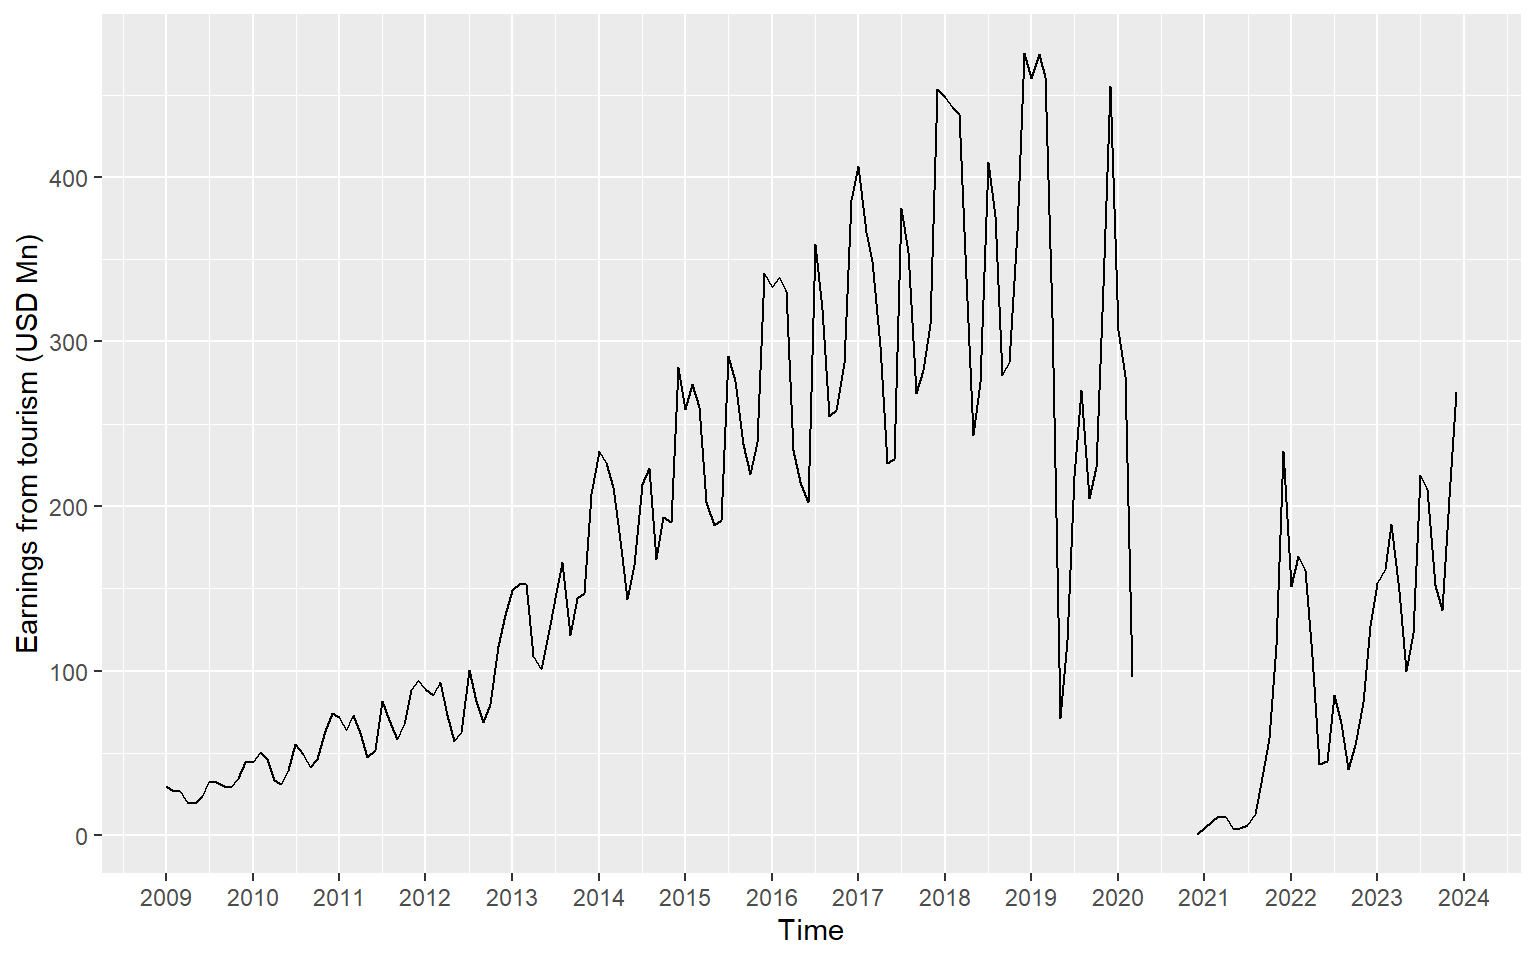
\includegraphics[keepaspectratio]{02-chap2_files/figure-pdf/unnamed-chunk-17-1.pdf}}

\begin{Shaded}
\begin{Highlighting}[]
\FunctionTok{library}\NormalTok{(viridis)}
\NormalTok{ts.earnings }\SpecialCharTok{|\textgreater{}}
  \FunctionTok{gg\_season}\NormalTok{(Earnings, }\AttributeTok{period =} \StringTok{"1 year"}\NormalTok{,  }\AttributeTok{pal =}\NormalTok{ scales}\SpecialCharTok{::}\FunctionTok{viridis\_pal}\NormalTok{()(}\DecValTok{15}\NormalTok{))  }\SpecialCharTok{+} \FunctionTok{geom\_point}\NormalTok{()  }
\end{Highlighting}
\end{Shaded}

\pandocbounded{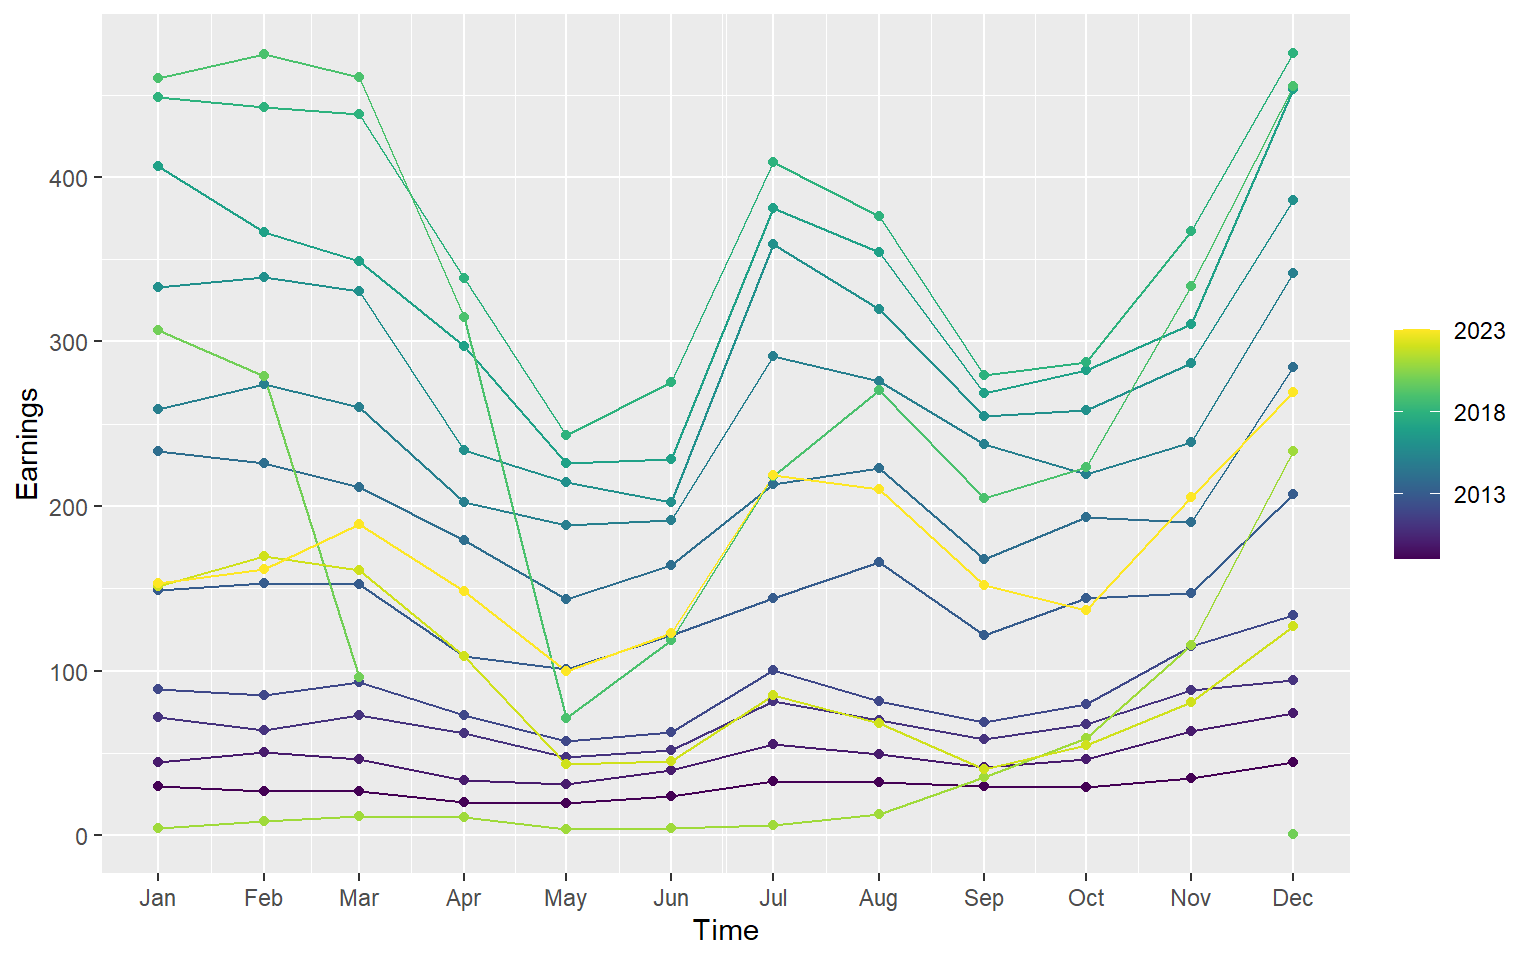
\includegraphics[keepaspectratio]{02-chap2_files/figure-pdf/unnamed-chunk-18-1.pdf}}

\section{Dataset: Python}\label{dataset-python}

\begin{Shaded}
\begin{Highlighting}[]
\ImportTok{import}\NormalTok{ plotnine }\ImportTok{as}\NormalTok{ p9}
\ImportTok{from}\NormalTok{ plotnine.data }\ImportTok{import}\NormalTok{ economics}
\end{Highlighting}
\end{Shaded}

\section{Working with Built-in Data
Set}\label{working-with-built-in-data-set}

\begin{Shaded}
\begin{Highlighting}[]
\ImportTok{import}\NormalTok{ pandas }\ImportTok{as}\NormalTok{ pd}
\ImportTok{import}\NormalTok{ plotnine }\ImportTok{as}\NormalTok{ p9 }
\ImportTok{from}\NormalTok{ plotnine }\ImportTok{import} \OperatorTok{*}
\ImportTok{from}\NormalTok{ plotnine.data }\ImportTok{import} \OperatorTok{*}
\ImportTok{import}\NormalTok{ numpy }\ImportTok{as}\NormalTok{ np}
\NormalTok{economics}
\end{Highlighting}
\end{Shaded}

\begin{verbatim}
          date      pce     pop  psavert  uempmed  unemploy
0   1967-07-01    507.4  198712     12.5      4.5      2944
1   1967-08-01    510.5  198911     12.5      4.7      2945
2   1967-09-01    516.3  199113     11.7      4.6      2958
3   1967-10-01    512.9  199311     12.5      4.9      3143
4   1967-11-01    518.1  199498     12.5      4.7      3066
..         ...      ...     ...      ...      ...       ...
569 2014-12-01  12122.0  320201      5.0     12.6      8688
570 2015-01-01  12080.8  320367      5.5     13.4      8979
571 2015-02-01  12095.9  320534      5.7     13.1      8705
572 2015-03-01  12161.5  320707      5.2     12.2      8575
573 2015-04-01  12158.9  320887      5.6     11.7      8549

[574 rows x 6 columns]
\end{verbatim}

\begin{Shaded}
\begin{Highlighting}[]
\NormalTok{economics.info()}
\end{Highlighting}
\end{Shaded}

\begin{verbatim}
<class 'pandas.core.frame.DataFrame'>
RangeIndex: 574 entries, 0 to 573
Data columns (total 6 columns):
 #   Column    Non-Null Count  Dtype         
---  ------    --------------  -----         
 0   date      574 non-null    datetime64[ns]
 1   pce       574 non-null    float64       
 2   pop       574 non-null    int64         
 3   psavert   574 non-null    float64       
 4   uempmed   574 non-null    float64       
 5   unemploy  574 non-null    int64         
dtypes: datetime64[ns](1), float64(3), int64(2)
memory usage: 27.0 KB
\end{verbatim}

\subsection{\texorpdfstring{Create \texttt{year} and \texttt{month}
columns}{Create year and month columns}}\label{create-year-and-month-columns}

\begin{Shaded}
\begin{Highlighting}[]
\NormalTok{economics[}\StringTok{\textquotesingle{}year\textquotesingle{}}\NormalTok{] }\OperatorTok{=}\NormalTok{ economics[}\StringTok{\textquotesingle{}date\textquotesingle{}}\NormalTok{].dt.year}
\NormalTok{economics[}\StringTok{\textquotesingle{}month\textquotesingle{}}\NormalTok{] }\OperatorTok{=}\NormalTok{ economics[}\StringTok{\textquotesingle{}date\textquotesingle{}}\NormalTok{].dt.month}
\NormalTok{economics}
\end{Highlighting}
\end{Shaded}

\begin{verbatim}
          date      pce     pop  psavert  uempmed  unemploy  year  month
0   1967-07-01    507.4  198712     12.5      4.5      2944  1967      7
1   1967-08-01    510.5  198911     12.5      4.7      2945  1967      8
2   1967-09-01    516.3  199113     11.7      4.6      2958  1967      9
3   1967-10-01    512.9  199311     12.5      4.9      3143  1967     10
4   1967-11-01    518.1  199498     12.5      4.7      3066  1967     11
..         ...      ...     ...      ...      ...       ...   ...    ...
569 2014-12-01  12122.0  320201      5.0     12.6      8688  2014     12
570 2015-01-01  12080.8  320367      5.5     13.4      8979  2015      1
571 2015-02-01  12095.9  320534      5.7     13.1      8705  2015      2
572 2015-03-01  12161.5  320707      5.2     12.2      8575  2015      3
573 2015-04-01  12158.9  320887      5.6     11.7      8549  2015      4

[574 rows x 8 columns]
\end{verbatim}

\section{Time series visualisation using grammar of graphics:
Python}\label{time-series-visualisation-using-grammar-of-graphics-python}

The grammar of graphics is a way of thinking about plots as layers. Each
plot is built from components like:

\textbf{Data} -- the dataset you are plotting.

\textbf{Aesthetics (aes)} -- how variables map to visual properties like
x, y, color, or size.

\textbf{Geometries (geom)} -- the type of plot (points, lines, bars,
etc.).

\textbf{Facets} -- split the plot into subplots based on a variable.

\textbf{Statistics (stat)} -- summary computations like regression lines
or counts.

\textbf{Scales} -- control axis limits, colors, or sizes.

\textbf{Coordinates (coord)} -- control coordinate system (Cartesian,
polar).

\textbf{Theme} -- control visual appearance like text, background, and
grid.

\href{https://thiyangt.github.io/spts_python_practical/Practical1/}{*}

\section{What is a lag value?}\label{what-is-a-lag-value}

In time series analysis, a lag represents the number of time steps by
which a series is shifted backward to compare it with itself.

Lag 1: Compare each value with the previous observation.

Lag 2: Compare each value with the value two steps before.

Lag k: Compare each value with the value k steps earlier.

\begin{Shaded}
\begin{Highlighting}[]
\ImportTok{import}\NormalTok{ pandas }\ImportTok{as}\NormalTok{ pd}

\CommentTok{\# Small time series with 5 points}
\NormalTok{data }\OperatorTok{=}\NormalTok{ [}\DecValTok{10}\NormalTok{, }\DecValTok{12}\NormalTok{, }\DecValTok{13}\NormalTok{, }\DecValTok{15}\NormalTok{, }\DecValTok{14}\NormalTok{]}
\NormalTok{dates }\OperatorTok{=}\NormalTok{ pd.date\_range(start}\OperatorTok{=}\StringTok{\textquotesingle{}2025{-}01{-}01\textquotesingle{}}\NormalTok{, periods}\OperatorTok{=}\DecValTok{5}\NormalTok{, freq}\OperatorTok{=}\StringTok{\textquotesingle{}D\textquotesingle{}}\NormalTok{)}

\NormalTok{df }\OperatorTok{=}\NormalTok{ pd.DataFrame(\{}\StringTok{\textquotesingle{}Date\textquotesingle{}}\NormalTok{: dates, }\StringTok{\textquotesingle{}Value\textquotesingle{}}\NormalTok{: data\})}
\NormalTok{df.set\_index(}\StringTok{\textquotesingle{}Date\textquotesingle{}}\NormalTok{, inplace}\OperatorTok{=}\VariableTok{True}\NormalTok{)}

\CommentTok{\# Create lagged series}
\NormalTok{df[}\StringTok{\textquotesingle{}Lag1\textquotesingle{}}\NormalTok{] }\OperatorTok{=}\NormalTok{ df[}\StringTok{\textquotesingle{}Value\textquotesingle{}}\NormalTok{].shift(}\DecValTok{1}\NormalTok{)  }\CommentTok{\# lag 1}
\NormalTok{df[}\StringTok{\textquotesingle{}Lag2\textquotesingle{}}\NormalTok{] }\OperatorTok{=}\NormalTok{ df[}\StringTok{\textquotesingle{}Value\textquotesingle{}}\NormalTok{].shift(}\DecValTok{2}\NormalTok{)  }\CommentTok{\# lag 2}

\CommentTok{\# Show the result}
\BuiltInTok{print}\NormalTok{(df)}
\end{Highlighting}
\end{Shaded}

\begin{verbatim}
            Value  Lag1  Lag2
Date                         
2025-01-01     10   NaN   NaN
2025-01-02     12  10.0   NaN
2025-01-03     13  12.0  10.0
2025-01-04     15  13.0  12.0
2025-01-05     14  15.0  13.0
\end{verbatim}

\section{Correlation vs
Autocorrelation}\label{correlation-vs-autocorrelation}

\subsection{Correlation}\label{correlation}

Measures the strength of the linear relationship between two variables

\[r = \frac{\sum_{i=1}^{n} (x_i -\bar{x})(y_i-\bar{y})}{\sqrt{\sum_{i=1}^{n} (x_i -\bar{x})^2 \sum_{i=1}^{n} (y_i -\bar{y})^2}}\]

\subsection{Autocorrelation}\label{autocorrelation}

Measures the strength of linear relationship between lagged values of
time series.

\[r_k = \frac{\sum (y_t -\bar{y})(y_{t-k}-\bar{y})}{\sum (y_t -\bar{y})^2}\]

\section{Your turn: why different
values?}\label{your-turn-why-different-values}

\begin{Shaded}
\begin{Highlighting}[]
\CommentTok{\# Correlation (autocorrelation) between original series and lagged series}
\NormalTok{autocorr\_lag1 }\OperatorTok{=}\NormalTok{ df[}\StringTok{\textquotesingle{}Value\textquotesingle{}}\NormalTok{].corr(df[}\StringTok{\textquotesingle{}Lag1\textquotesingle{}}\NormalTok{])}
\NormalTok{autocorr\_lag2 }\OperatorTok{=}\NormalTok{ df[}\StringTok{\textquotesingle{}Value\textquotesingle{}}\NormalTok{].corr(df[}\StringTok{\textquotesingle{}Lag2\textquotesingle{}}\NormalTok{])}

\BuiltInTok{print}\NormalTok{(}\SpecialStringTok{f"Autocorrelation at lag 1: }\SpecialCharTok{\{}\NormalTok{autocorr\_lag1}\SpecialCharTok{:.3f\}}\SpecialStringTok{"}\NormalTok{)}
\end{Highlighting}
\end{Shaded}

\begin{verbatim}
Autocorrelation at lag 1: 0.744
\end{verbatim}

\begin{Shaded}
\begin{Highlighting}[]
\BuiltInTok{print}\NormalTok{(}\SpecialStringTok{f"Autocorrelation at lag 2: }\SpecialCharTok{\{}\NormalTok{autocorr\_lag2}\SpecialCharTok{:.3f\}}\SpecialStringTok{"}\NormalTok{)}
\end{Highlighting}
\end{Shaded}

\begin{verbatim}
Autocorrelation at lag 2: 0.655
\end{verbatim}

\begin{Shaded}
\begin{Highlighting}[]
\ImportTok{import}\NormalTok{ pandas }\ImportTok{as}\NormalTok{ pd}
\ImportTok{import}\NormalTok{ numpy }\ImportTok{as}\NormalTok{ np}
\ImportTok{import}\NormalTok{ matplotlib.pyplot }\ImportTok{as}\NormalTok{ plt}
\ImportTok{from}\NormalTok{ statsmodels.tsa.stattools }\ImportTok{import}\NormalTok{ acf}

\CommentTok{\# Small time series with 5 points}
\NormalTok{data }\OperatorTok{=}\NormalTok{ [}\DecValTok{10}\NormalTok{, }\DecValTok{12}\NormalTok{, }\DecValTok{13}\NormalTok{, }\DecValTok{15}\NormalTok{, }\DecValTok{14}\NormalTok{]}
\NormalTok{dates }\OperatorTok{=}\NormalTok{ pd.date\_range(start}\OperatorTok{=}\StringTok{\textquotesingle{}2025{-}01{-}01\textquotesingle{}}\NormalTok{, periods}\OperatorTok{=}\DecValTok{5}\NormalTok{, freq}\OperatorTok{=}\StringTok{\textquotesingle{}D\textquotesingle{}}\NormalTok{)}

\NormalTok{df }\OperatorTok{=}\NormalTok{ pd.DataFrame(\{}\StringTok{\textquotesingle{}Date\textquotesingle{}}\NormalTok{: dates, }\StringTok{\textquotesingle{}Value\textquotesingle{}}\NormalTok{: data\})}
\NormalTok{df.set\_index(}\StringTok{\textquotesingle{}Date\textquotesingle{}}\NormalTok{, inplace}\OperatorTok{=}\VariableTok{True}\NormalTok{)}

\BuiltInTok{print}\NormalTok{(df)}
\end{Highlighting}
\end{Shaded}

\begin{verbatim}
            Value
Date             
2025-01-01     10
2025-01-02     12
2025-01-03     13
2025-01-04     15
2025-01-05     14
\end{verbatim}

\begin{Shaded}
\begin{Highlighting}[]
\CommentTok{\# Compute autocorrelation for lags 1 to 4 (max lag = n{-}1)}
\NormalTok{autocorr\_values }\OperatorTok{=}\NormalTok{ acf(df[}\StringTok{\textquotesingle{}Value\textquotesingle{}}\NormalTok{], nlags}\OperatorTok{=}\DecValTok{4}\NormalTok{, fft}\OperatorTok{=}\VariableTok{False}\NormalTok{)}

\CommentTok{\# Show autocorrelation values}
\ControlFlowTok{for}\NormalTok{ lag, val }\KeywordTok{in} \BuiltInTok{enumerate}\NormalTok{(autocorr\_values):}
    \BuiltInTok{print}\NormalTok{(}\SpecialStringTok{f"Lag }\SpecialCharTok{\{}\NormalTok{lag}\SpecialCharTok{\}}\SpecialStringTok{: }\SpecialCharTok{\{}\NormalTok{val}\SpecialCharTok{:.3f\}}\SpecialStringTok{"}\NormalTok{)}
\end{Highlighting}
\end{Shaded}

\begin{verbatim}
Lag 0: 1.000
Lag 1: 0.349
Lag 2: -0.141
Lag 3: -0.481
Lag 4: -0.227
\end{verbatim}

\section{Autocorrelation plots (ACF)}\label{autocorrelation-plots-acf}

The ACF measures the correlation between a time series and lagged
versions of itself. It tells us how past values influence current
values.

\subsection{Example 1}\label{example-1}

Time series plot

\begin{Shaded}
\begin{Highlighting}[]
\FunctionTok{library}\NormalTok{(fable)}
\FunctionTok{library}\NormalTok{(fpp2)}
\FunctionTok{autoplot}\NormalTok{(beer)}
\end{Highlighting}
\end{Shaded}

\pandocbounded{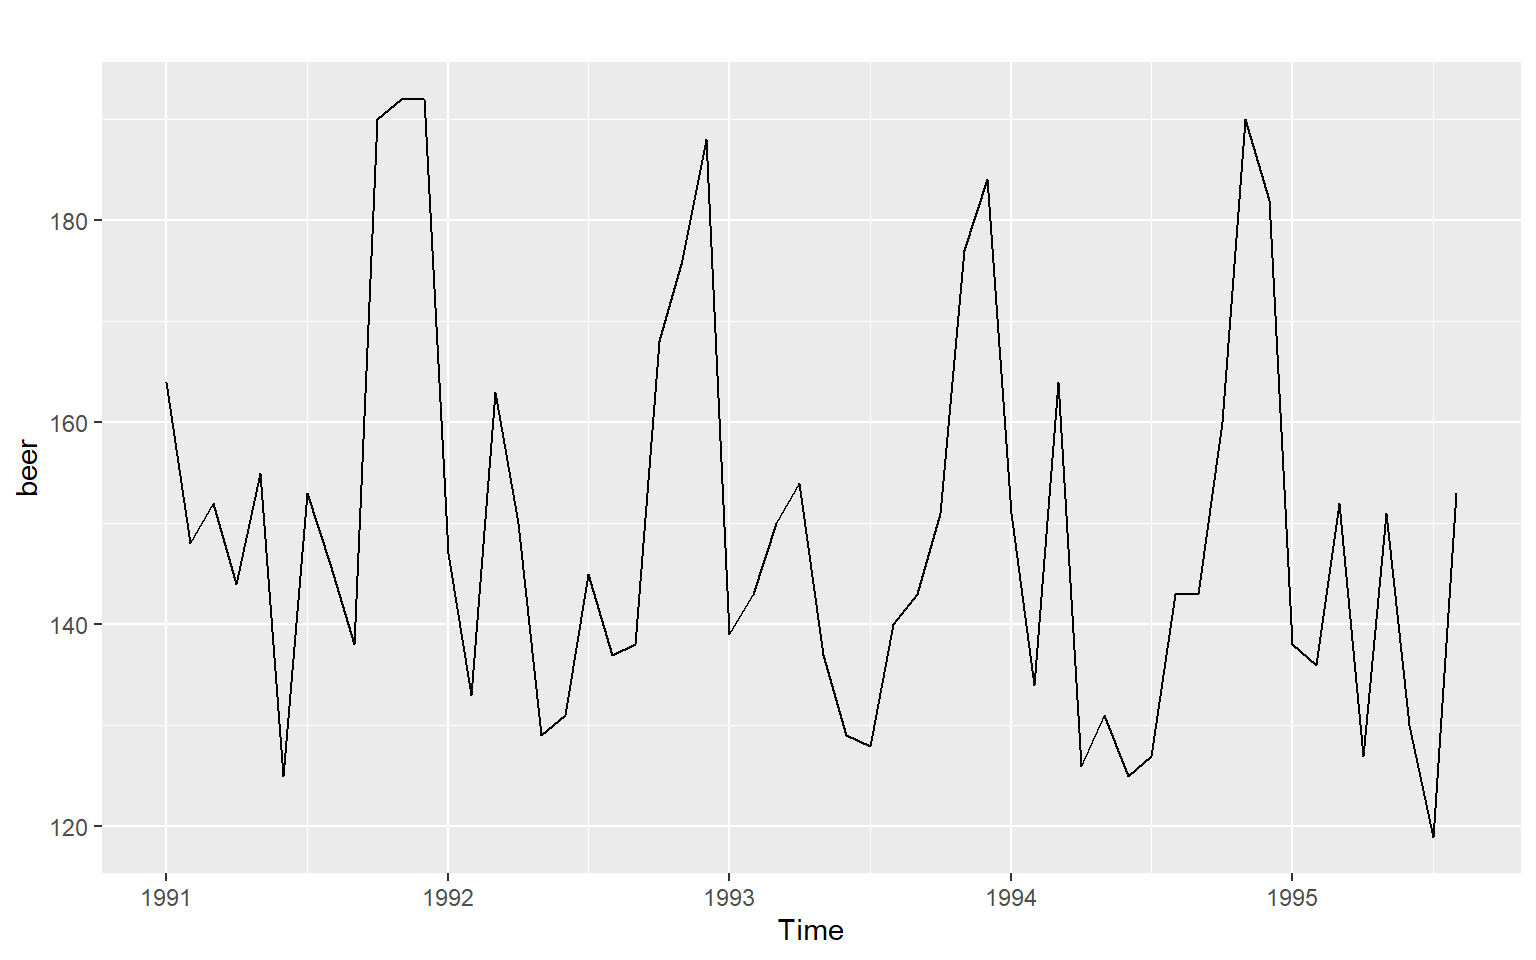
\includegraphics[keepaspectratio]{02-chap2_files/figure-pdf/unnamed-chunk-27-1.pdf}}

Seasonal plot

\begin{Shaded}
\begin{Highlighting}[]
\FunctionTok{ggseasonplot}\NormalTok{(beer, }\AttributeTok{year.labels=}\ConstantTok{TRUE}\NormalTok{, }\AttributeTok{year.labels.left=}\ConstantTok{TRUE}\NormalTok{)}
\end{Highlighting}
\end{Shaded}

\pandocbounded{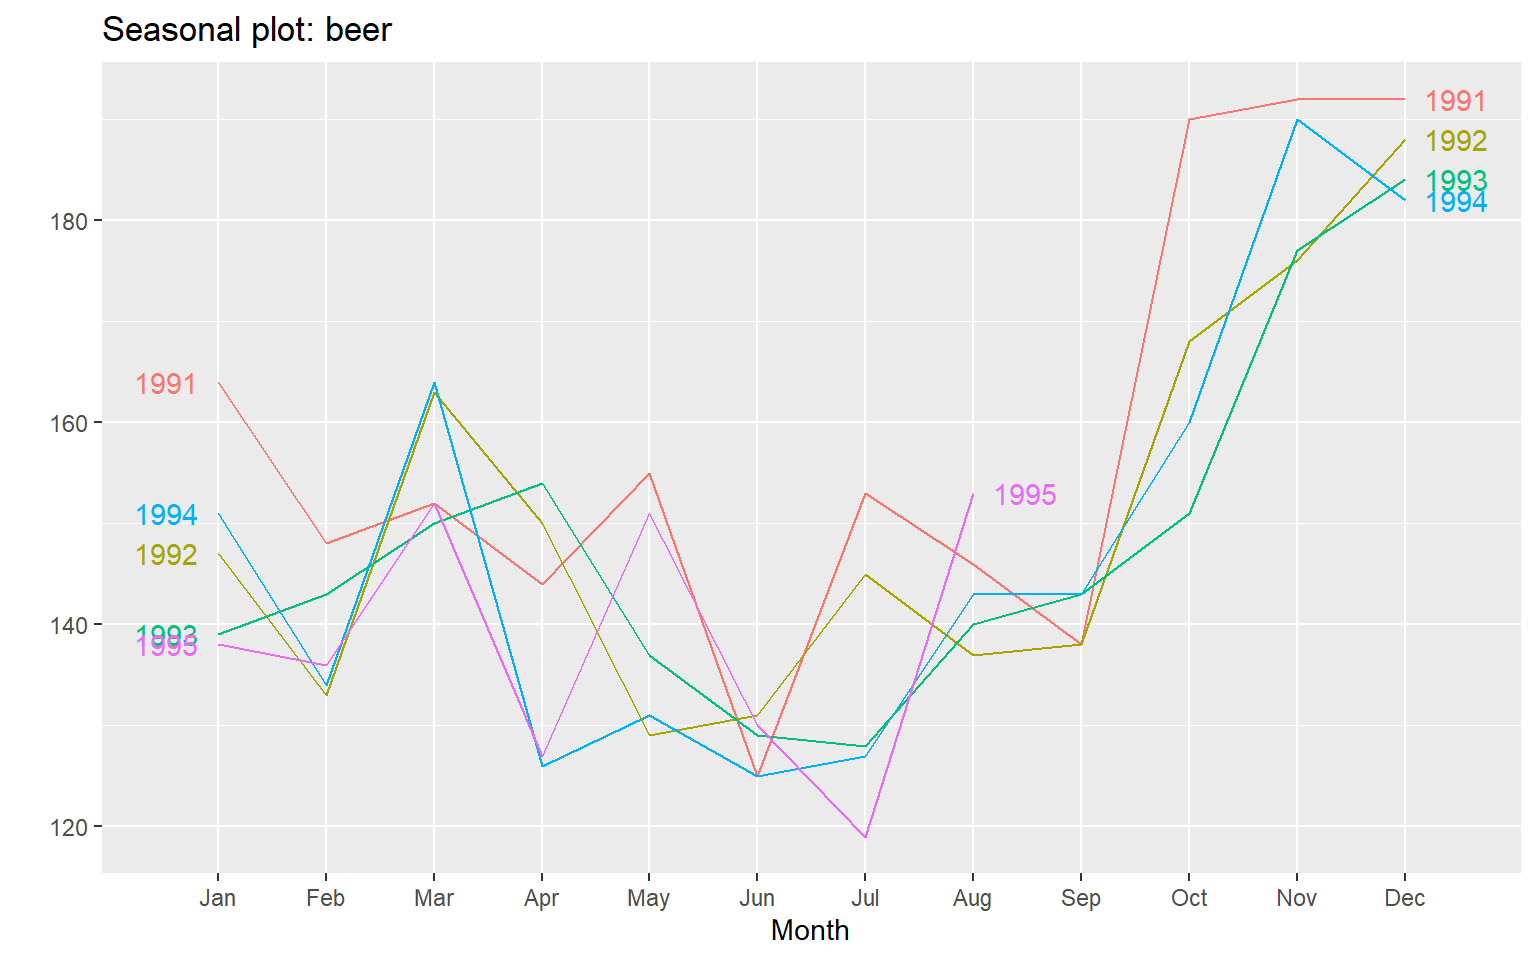
\includegraphics[keepaspectratio]{02-chap2_files/figure-pdf/unnamed-chunk-28-1.pdf}}

ACF

\begin{Shaded}
\begin{Highlighting}[]
\FunctionTok{ggAcf}\NormalTok{(beer)}
\end{Highlighting}
\end{Shaded}

\pandocbounded{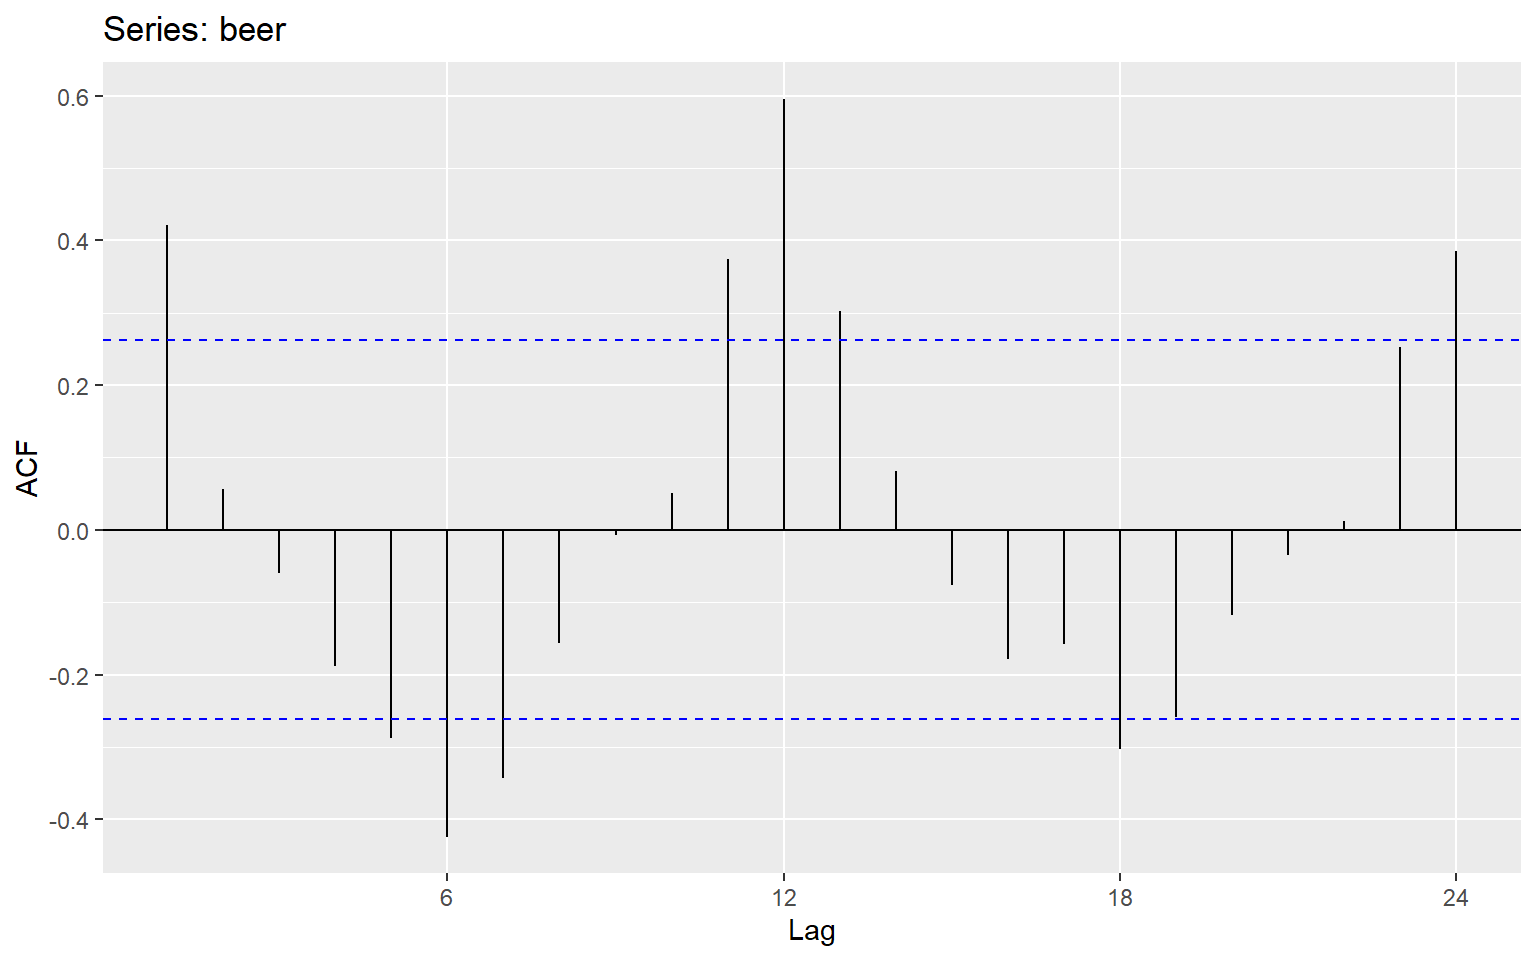
\includegraphics[keepaspectratio]{02-chap2_files/figure-pdf/unnamed-chunk-29-1.pdf}}

\begin{Shaded}
\begin{Highlighting}[]
\FunctionTok{ggseasonplot}\NormalTok{(beer, }\AttributeTok{year.labels=}\ConstantTok{TRUE}\NormalTok{, }\AttributeTok{year.labels.left=}\ConstantTok{TRUE}\NormalTok{)}
\end{Highlighting}
\end{Shaded}

\pandocbounded{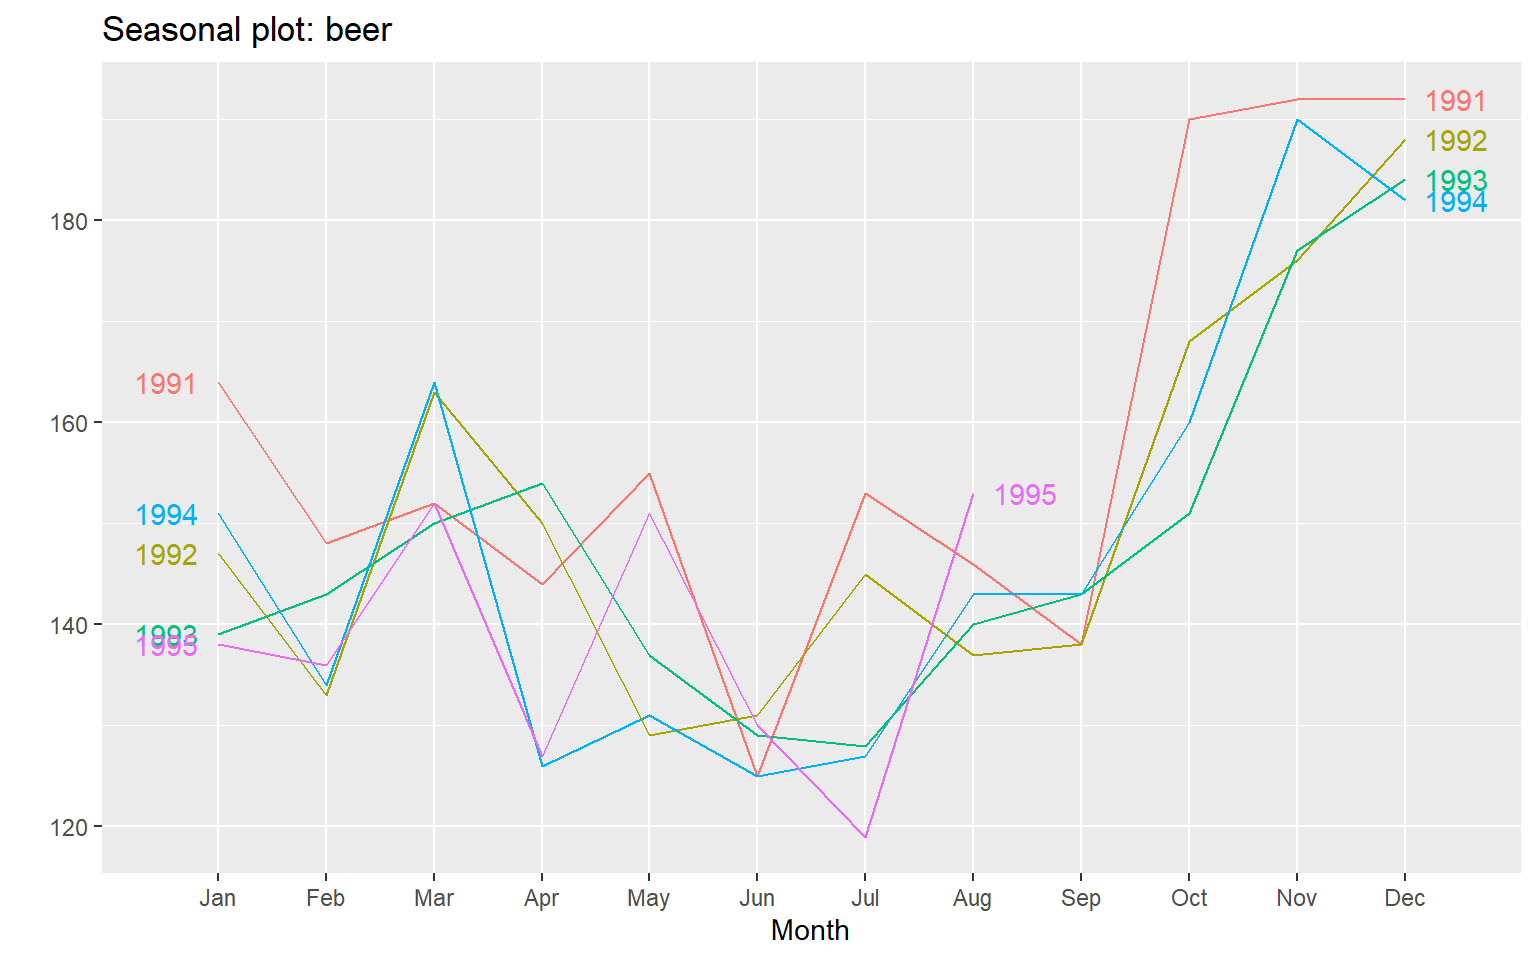
\includegraphics[keepaspectratio]{02-chap2_files/figure-pdf/unnamed-chunk-30-1.pdf}}

\section{Example 2}\label{example-2}

\begin{Shaded}
\begin{Highlighting}[]
\NormalTok{aelec }\OtherTok{\textless{}{-}} \FunctionTok{window}\NormalTok{(elec, }\AttributeTok{start=}\DecValTok{1980}\NormalTok{)}
\FunctionTok{autoplot}\NormalTok{(aelec) }\SpecialCharTok{+} \FunctionTok{xlab}\NormalTok{(}\StringTok{"Year"}\NormalTok{) }\SpecialCharTok{+} \FunctionTok{ylab}\NormalTok{(}\StringTok{"GWh"}\NormalTok{)}
\end{Highlighting}
\end{Shaded}

\pandocbounded{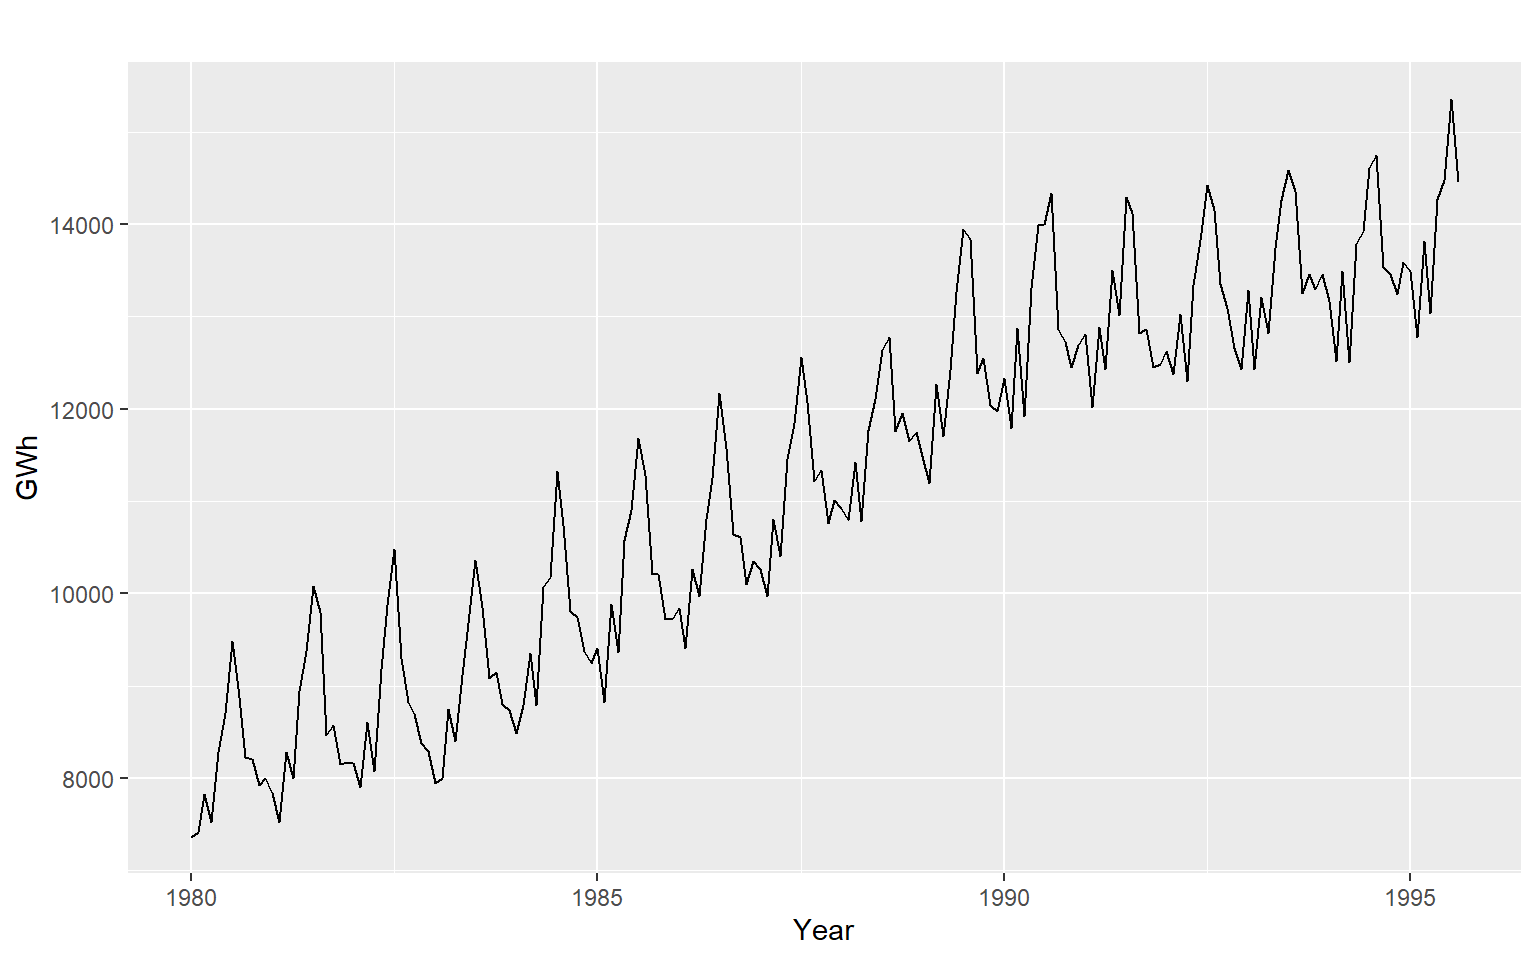
\includegraphics[keepaspectratio]{02-chap2_files/figure-pdf/unnamed-chunk-31-1.pdf}}

Seasonal plots

\begin{Shaded}
\begin{Highlighting}[]
\FunctionTok{ggseasonplot}\NormalTok{(aelec, }\AttributeTok{year.labels=}\ConstantTok{TRUE}\NormalTok{, }\AttributeTok{year.labels.left=}\ConstantTok{TRUE}\NormalTok{)}
\end{Highlighting}
\end{Shaded}

\pandocbounded{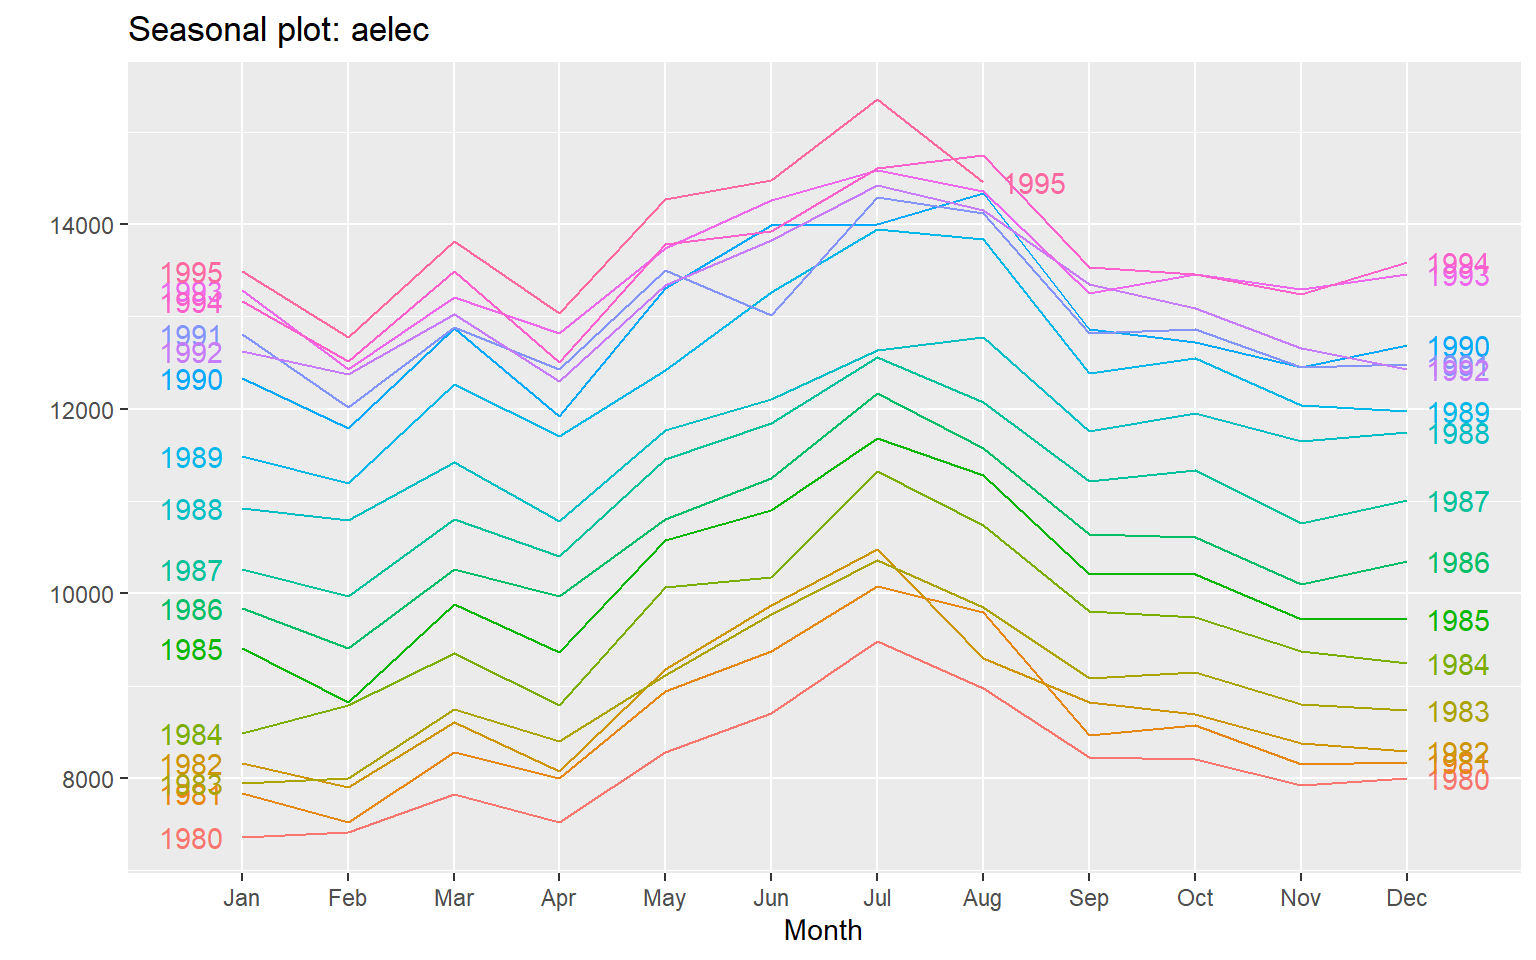
\includegraphics[keepaspectratio]{02-chap2_files/figure-pdf/unnamed-chunk-32-1.pdf}}

\begin{Shaded}
\begin{Highlighting}[]
\FunctionTok{ggAcf}\NormalTok{(aelec, }\AttributeTok{lag=}\DecValTok{48}\NormalTok{)}
\end{Highlighting}
\end{Shaded}

\pandocbounded{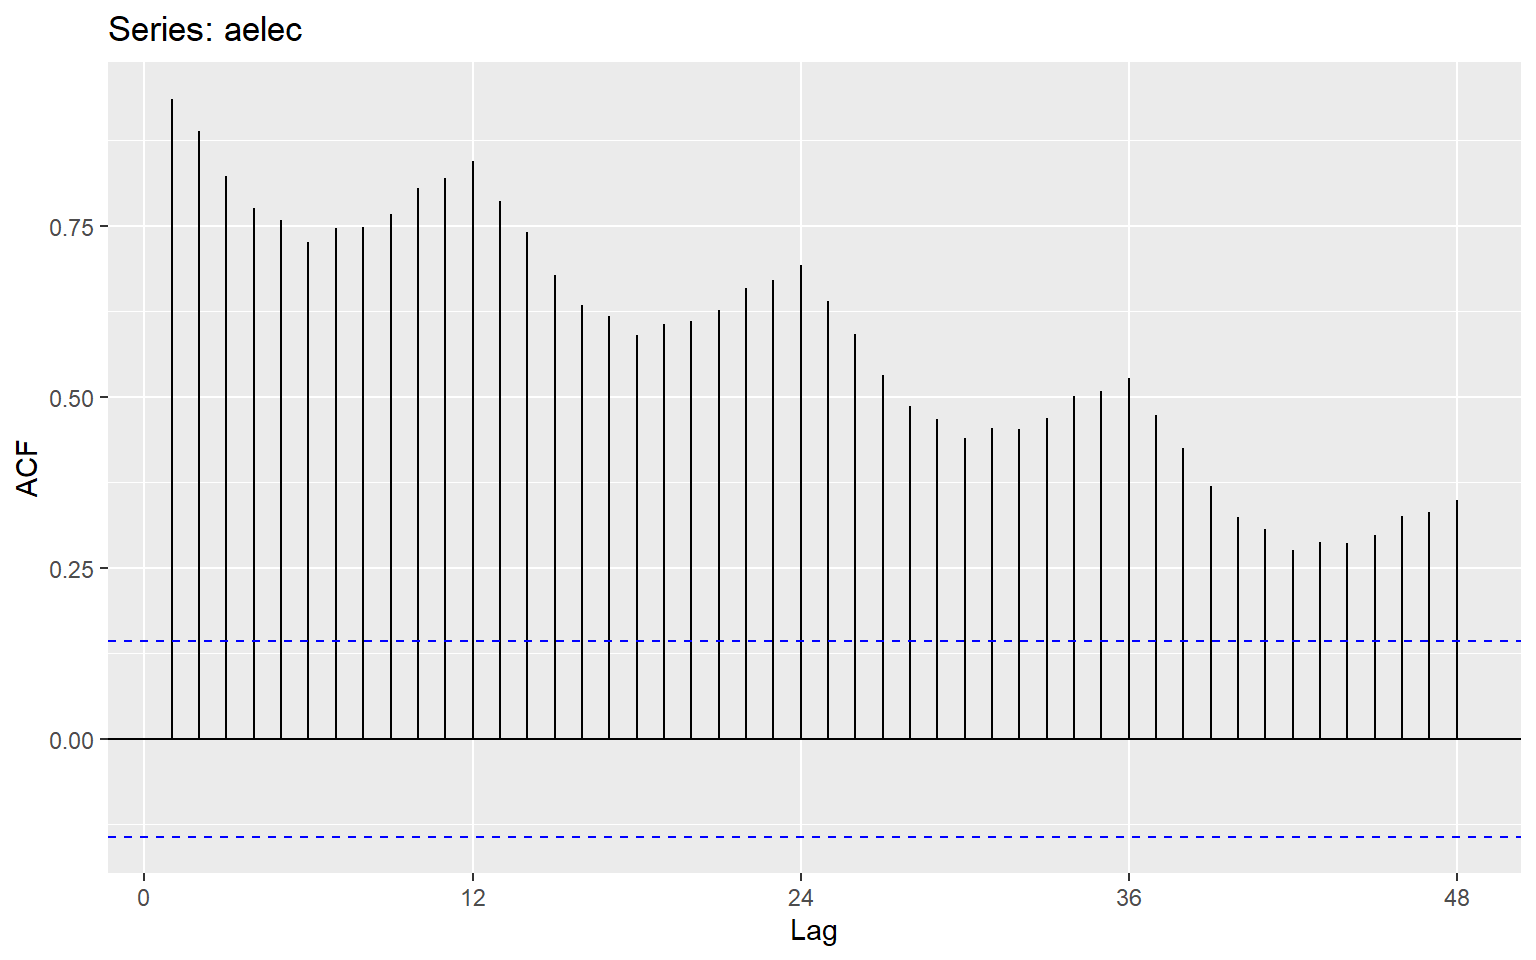
\includegraphics[keepaspectratio]{02-chap2_files/figure-pdf/unnamed-chunk-33-1.pdf}}

\section{Example 3}\label{example-3}

\begin{Shaded}
\begin{Highlighting}[]
\FunctionTok{set.seed}\NormalTok{(}\DecValTok{3}\NormalTok{)}
\NormalTok{y }\OtherTok{\textless{}{-}} \FunctionTok{ts}\NormalTok{(}\FunctionTok{rnorm}\NormalTok{(}\DecValTok{50}\NormalTok{))}
\FunctionTok{autoplot}\NormalTok{(y) }\SpecialCharTok{+} \FunctionTok{ggtitle}\NormalTok{(}\StringTok{"White noise"}\NormalTok{)}
\end{Highlighting}
\end{Shaded}

\pandocbounded{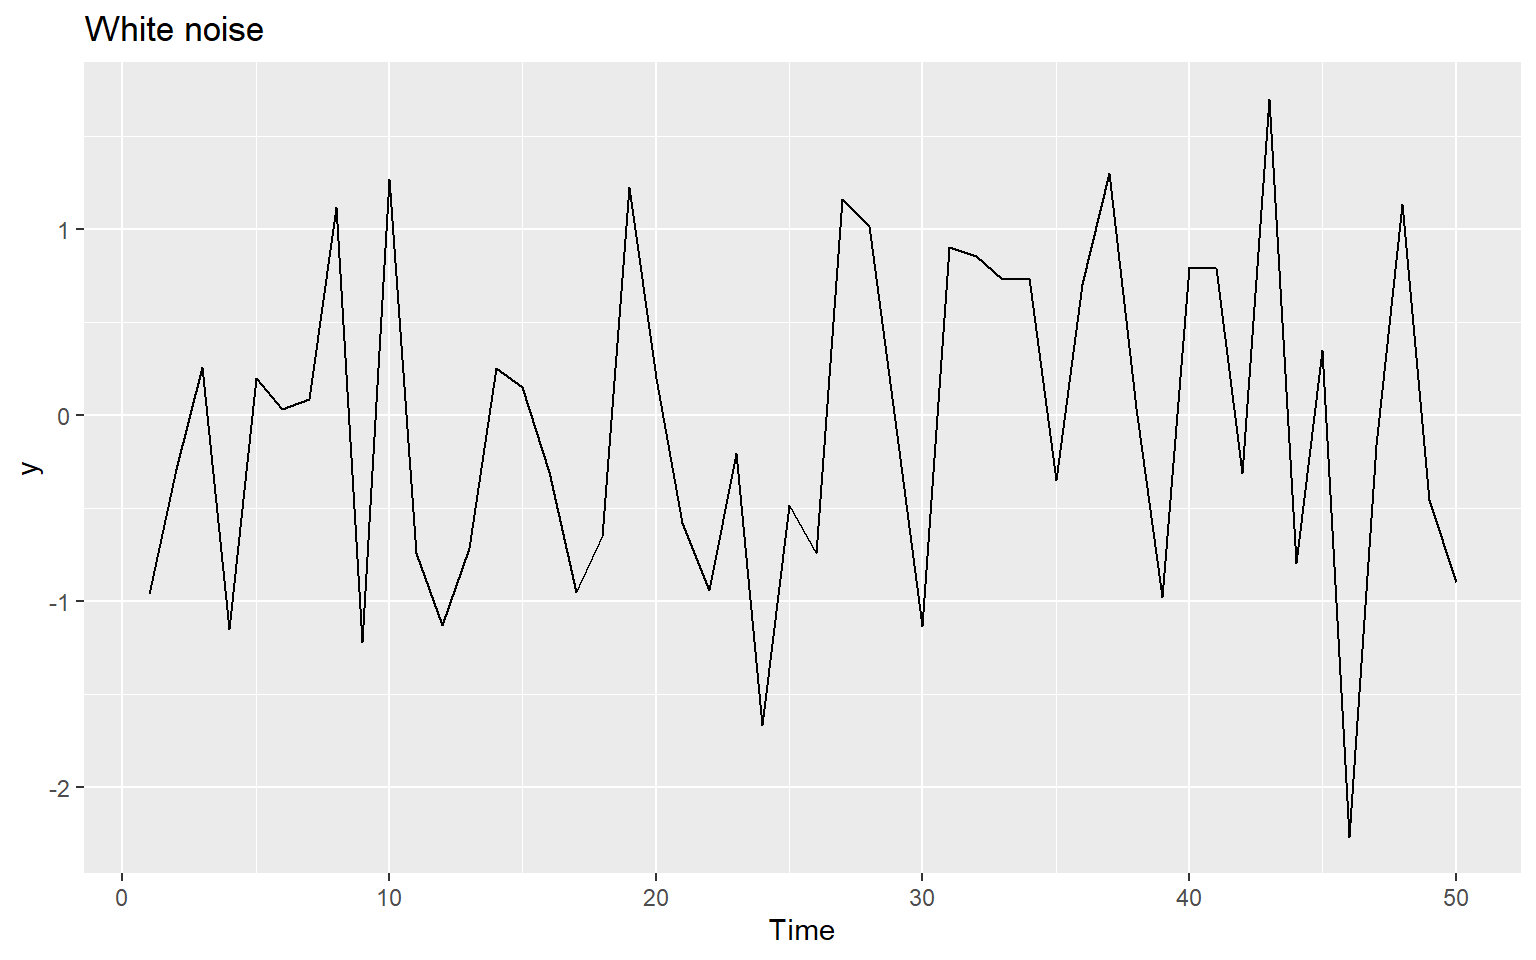
\includegraphics[keepaspectratio]{02-chap2_files/figure-pdf/unnamed-chunk-34-1.pdf}}

\begin{Shaded}
\begin{Highlighting}[]
\FunctionTok{ggAcf}\NormalTok{(y)}
\end{Highlighting}
\end{Shaded}

\pandocbounded{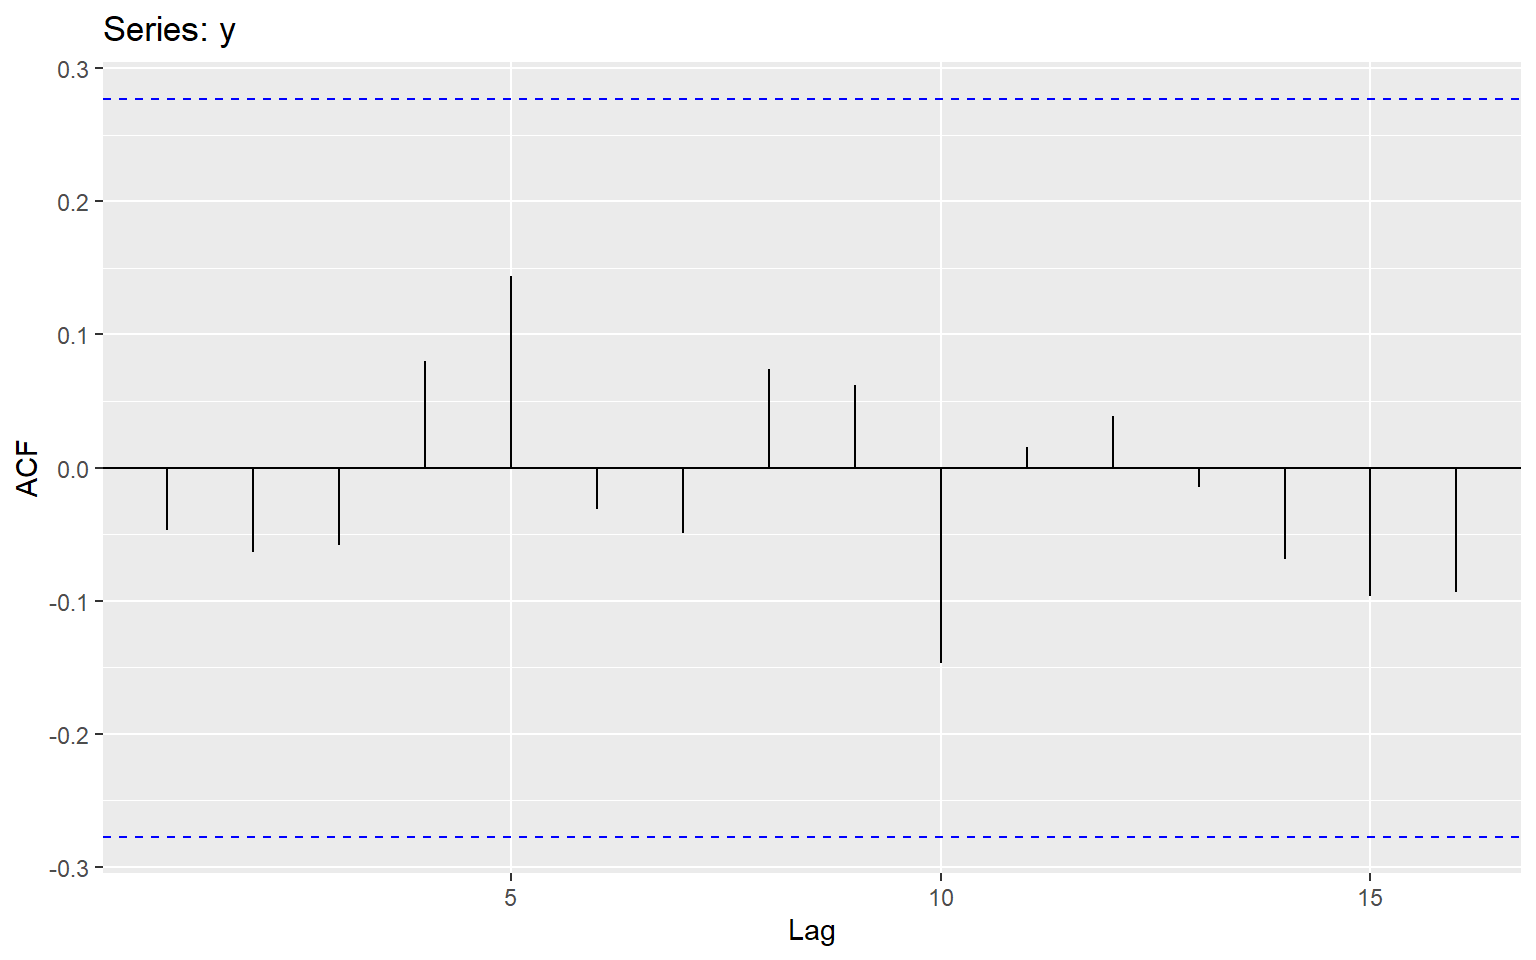
\includegraphics[keepaspectratio]{02-chap2_files/figure-pdf/unnamed-chunk-35-1.pdf}}

\section{Exercise}\label{exercise}

Question 6 at \url{https://otexts.com/fpp2/graphics-exercises.html}

\bookmarksetup{startatroot}

\chapter{Introduction to Time Series
Forecasting}\label{introduction-to-time-series-forecasting}

\section{Notation}\label{notation}

\(\hat{Y}_{T+h|T}\) - The forecast of the time series \(𝑌\) at time
\(T+h\), made using the information available up to time \(T\).

\section{Simple time series forecasting
techniques}\label{simple-time-series-forecasting-techniques}

\begin{enumerate}
\def\labelenumi{\arabic{enumi}.}
\item
  Average method
\item
  Naive method/ random walk method
\item
  Seasonal naive method
\item
  Drift method
\end{enumerate}

\href{https://otexts.com/fpp2/simple-methods.html}{Reading}

\section{Example: Electricity Demand
Forecasting}\label{example-electricity-demand-forecasting}

\begin{Shaded}
\begin{Highlighting}[]
\FunctionTok{library}\NormalTok{(fable)}
\FunctionTok{library}\NormalTok{(fpp2)}
\end{Highlighting}
\end{Shaded}

\begin{Shaded}
\begin{Highlighting}[]
\NormalTok{aelec }\OtherTok{\textless{}{-}} \FunctionTok{window}\NormalTok{(elec, }\AttributeTok{start=}\DecValTok{1980}\NormalTok{)}
\FunctionTok{autoplot}\NormalTok{(aelec)}
\end{Highlighting}
\end{Shaded}

\pandocbounded{\includegraphics[keepaspectratio]{03-chap3_files/figure-pdf/unnamed-chunk-3-1.pdf}}

\begin{Shaded}
\begin{Highlighting}[]
\CommentTok{\# Plot some forecasts}
\FunctionTok{autoplot}\NormalTok{(aelec) }\SpecialCharTok{+}
  \FunctionTok{autolayer}\NormalTok{(}\FunctionTok{meanf}\NormalTok{(aelec, }\AttributeTok{h=}\DecValTok{11}\NormalTok{),}
    \AttributeTok{series=}\StringTok{"Mean"}\NormalTok{, }\AttributeTok{PI=}\ConstantTok{FALSE}\NormalTok{) }\SpecialCharTok{+}
  \FunctionTok{autolayer}\NormalTok{(}\FunctionTok{naive}\NormalTok{(aelec, }\AttributeTok{h=}\DecValTok{11}\NormalTok{),}
    \AttributeTok{series=}\StringTok{"Naïve"}\NormalTok{, }\AttributeTok{PI=}\ConstantTok{FALSE}\NormalTok{) }\SpecialCharTok{+}
  \FunctionTok{autolayer}\NormalTok{(}\FunctionTok{snaive}\NormalTok{(aelec, }\AttributeTok{h=}\DecValTok{11}\NormalTok{),}
    \AttributeTok{series=}\StringTok{"Seasonal naïve"}\NormalTok{, }\AttributeTok{PI=}\ConstantTok{FALSE}\NormalTok{) }\SpecialCharTok{+}
  \FunctionTok{ggtitle}\NormalTok{(}\StringTok{"Forecasts from Mean, NAIVE and SNAIVE"}\NormalTok{) }\SpecialCharTok{+}
  \FunctionTok{xlab}\NormalTok{(}\StringTok{"Year"}\NormalTok{) }\SpecialCharTok{+} \FunctionTok{ylab}\NormalTok{(}\StringTok{"Value"}\NormalTok{) }\SpecialCharTok{+}
  \FunctionTok{guides}\NormalTok{(}\AttributeTok{colour=}\FunctionTok{guide\_legend}\NormalTok{(}\AttributeTok{title=}\StringTok{"Forecast"}\NormalTok{))}
\end{Highlighting}
\end{Shaded}

\pandocbounded{\includegraphics[keepaspectratio]{03-chap3_files/figure-pdf/unnamed-chunk-4-1.pdf}}

\section{Time Series and Stochastic
Processes}\label{time-series-and-stochastic-processes}

The terms stochastic processes and time series are closely related but
not the same.

A \textbf{stochastic process} is a collection of random variables
indexed by time (or space).

\[\{X_t : t \in T\},\]

where \(T\) is the index set (e.g., discrete or continuous time).

A \textbf{time series} is a single realization (observed data) of a
stochastic process. It is the actual sequence of observations collected
over time.

In short:

Stochastic process = model/theory (all possible sequences). The
probability mechanism (all possible paths).

Time series = observed data (one sequence). One observed path (the
single trajectory we actually have).

\section{Statistical Properties}\label{statistical-properties}

\subsection{Mean function}\label{mean-function}

Let \({X_1, X_2, ...}\) be a sequence of time index random variables.

The \textbf{mean function} of \({X_t}\) is

\[\mu_X(t)=E(X_t).\]

\subsection{Covariance function}\label{covariance-function}

The \textbf{covariance function} of \({X_t}\) is

\[\gamma_X(r, s)=Cov(X_r, X_s)=E[(X_r-\mu_X(r))(X_s-\mu_X(s))]\]

for all integers \((r)\) and \((s)\).

\subsection{Autocovariance function}\label{autocovariance-function}

The autocovariance function of \({X_t}\) at lag \((h)\) is defined by
\[\gamma_X(h):=\gamma_X(h, 0)=\gamma(t+h, t)=Cov(X_{t+h}, X_t).\]

or

The autocovariance function of \({X_t}\) at lag \((h)\) is

\[\gamma_X(h)=Cov(X_{t+h}, X_t).\]

\subsection{Autocorrelation function}\label{autocorrelation-function}

The autocorrelation function of \({X_t}\) at lag \((h)\) is

\[\rho_X(h)=\frac{\gamma_X(h)}{\gamma_X(0)}=Cor(X_{t+h}, X_t).\]

\section{Weakly stationary}\label{weakly-stationary}

A time series \({X_t}\) is called weakly stationary if

\begin{itemize}
\item
  \(\mu_X(t)\) is independent of \(t\).
\item
  \(Var(X_t) = \sigma^2\), Variance is constant. 2
\item
  \(\gamma_X(t+h, t)\) is independent of \((t)\) for each \((h)\). The
  autocovariance depends only on the lag (\(\gamma(h)\) depends only on
  how far apart two points are (\(h\)), and not on the actual time
  \(t\).
\end{itemize}

In other words the statistical properties of the time series (mean,
variance, autocorrelation, etc.) do not depend on the time at which the
series is observed, that is no trend or seasonality. However, a time
series with cyclic behaviour (but with no trend or seasonality) is
stationary.

\section{Strict stationarity of a time
series}\label{strict-stationarity-of-a-time-series}

A time series \(\{X_t\}\) is called strictly stationary if the random
vector \([X_1, X_2..., X_n]\) and \([X_{1+h}, X_{2+h}..., X_{n+h}]\)
have the same joint distribution for all integers \((h)\) and
\((n > 0)\).

\section{1. independent and identically distributed (iid)
noise}\label{independent-and-identically-distributed-iid-noise}

\begin{enumerate}
\def\labelenumi{\arabic{enumi}.}
\item
  no trend or seasonal component
\item
  observations are independent and identically distributed (iid) random
  variables with zero mean.
\item
  Notation: \({X_t} \sim IID(0, \sigma^2)\)
\item
  plays an important role as a building block for more complicated time
  series.
\end{enumerate}

\section{2. White noise}\label{white-noise}

If \({X_t}\) is a sequence of uncorrelated random variables, each with
zero mean and variance \(\sigma^2\), then such a sequence is referred to
as \textbf{white noise}.

\section{\texorpdfstring{Every \((IID(0, \sigma^2)\) sequence is
\((WN(0, \sigma^2)\) but not conversely.
Why?}{Every (IID(0, \textbackslash sigma\^{}2) sequence is (WN(0, \textbackslash sigma\^{}2) but not conversely. Why?}}\label{every-iid0-sigma2-sequence-is-wn0-sigma2-but-not-conversely.-why}

\subsection{1. White Noise (WN)}\label{white-noise-wn}

A sequence \(\{X_t\}\) is called \textbf{white noise} with mean \(0\)
and variance \(\sigma^2\), written \(WN(0, \sigma^2)\), if:

\begin{itemize}
\tightlist
\item
  \(\mathbb{E}[X_t] = 0\) for all \(t\).\\
\item
  \(\mathrm{Var}(X_t) = \sigma^2\) for all \(t\).\\
\item
  \(\mathrm{Cov}(X_t, X_s) = 0\) for all \(t \neq s\) (uncorrelated
  across time).
\end{itemize}

Notice: \emph{uncorrelated \(\neq\) independent}.

\subsection{\texorpdfstring{2. i.i.d.
\((0, \sigma^2)\)}{2. i.i.d. (0, \textbackslash sigma\^{}2)}}\label{i.i.d.-0-sigma2}

A sequence \(\{X_t\}\) is \(IID(0, \sigma^2)\) if:

\begin{itemize}
\tightlist
\item
  \(\mathbb{E}[X_t] = 0\).\\
\item
  \(\mathrm{Var}(X_t) = \sigma^2\).\\
\item
  \(X_t\) are independent and identically distributed.
\end{itemize}

\subsection{\texorpdfstring{3. Why every \(IID(0, \sigma^2)\) is
\(WN(0, \sigma^2)\)}{3. Why every IID(0, \textbackslash sigma\^{}2) is WN(0, \textbackslash sigma\^{}2)}}\label{why-every-iid0-sigma2-is-wn0-sigma2}

\begin{itemize}
\tightlist
\item
  Independence \(\;\Rightarrow\;\) zero correlation.\\
\item
  So, an i.i.d. sequence automatically satisfies the white noise
  conditions (same mean, same variance, no correlation).
\end{itemize}

Therefore:

\[
IID(0, \sigma^2) \;\;\Rightarrow\;\; WN(0, \sigma^2).
\]

\subsection{4. Why not conversely?}\label{why-not-conversely}

The reverse is not always true, because \textbf{white noise only
requires uncorrelatedness, not full independence}.

That means a sequence could be white noise but still have dependence in
higher moments (nonlinear dependence).

\section{5. Example of WN but not IID}\label{example-of-wn-but-not-iid}

Let \(\{Z_t\}\) be i.i.d. \(N(0,1)\). Define

\[
X_t = Z_t \cdot Z_{t-1}.
\]

Then:

\begin{itemize}
\tightlist
\item
  \(\mathbb{E}[X_t] = 0\),\\
\item
  \(\mathrm{Var}(X_t) = 1\),\\
\item
  For \(t \neq s\), \(\mathrm{Cov}(X_t, X_s) = 0\). ✅ So it's white
  noise.
\end{itemize}

But the sequence is \textbf{not independent} (because \(X_t\) depends on
\(Z_{t-1}\), which also appears in \(X_{t-1}\)).

Thus,

\[
X_t \sim WN(0,1) \quad \text{but not} \quad IID(0,1).
\]

\section{Simulation example}\label{simulation-example}

IID series

\begin{Shaded}
\begin{Highlighting}[]
\FunctionTok{set.seed}\NormalTok{(}\DecValTok{123}\NormalTok{)}

\CommentTok{\# Parameters}
\NormalTok{n }\OtherTok{\textless{}{-}} \DecValTok{200}        \CommentTok{\# length of series}
\NormalTok{sigma }\OtherTok{\textless{}{-}} \DecValTok{1}      \CommentTok{\# standard deviation}

\CommentTok{\# IID(0, sigma\^{}2) \textasciitilde{} Normal(0, sigma\^{}2)}
\NormalTok{iid\_seq }\OtherTok{\textless{}{-}} \FunctionTok{rnorm}\NormalTok{(n, }\AttributeTok{mean =} \DecValTok{0}\NormalTok{, }\AttributeTok{sd =}\NormalTok{ sigma)}

\CommentTok{\# Quick check}
\FunctionTok{mean}\NormalTok{(iid\_seq)      }\CommentTok{\# should be \textasciitilde{}0}
\end{Highlighting}
\end{Shaded}

\begin{verbatim}
[1] -0.008570445
\end{verbatim}

\begin{Shaded}
\begin{Highlighting}[]
\FunctionTok{var}\NormalTok{(iid\_seq)       }\CommentTok{\# should be \textasciitilde{}sigma\^{}2}
\end{Highlighting}
\end{Shaded}

\begin{verbatim}
[1] 0.8895506
\end{verbatim}

\begin{Shaded}
\begin{Highlighting}[]
\FunctionTok{acf}\NormalTok{(iid\_seq)       }\CommentTok{\# autocorrelations \textasciitilde{} 0}
\end{Highlighting}
\end{Shaded}

\pandocbounded{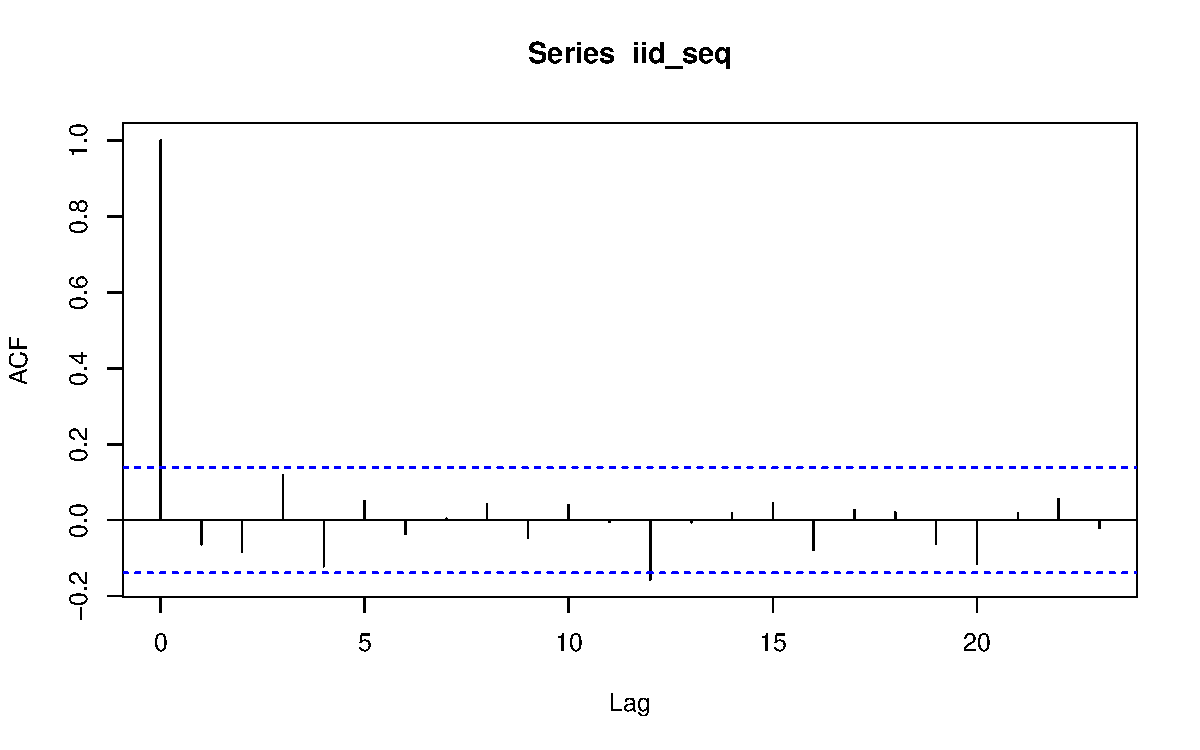
\includegraphics[keepaspectratio]{03-chap3_files/figure-pdf/unnamed-chunk-5-1.pdf}}

White noise

\begin{Shaded}
\begin{Highlighting}[]
\FunctionTok{set.seed}\NormalTok{(}\DecValTok{123}\NormalTok{)}

\NormalTok{n }\OtherTok{\textless{}{-}} \DecValTok{200}
\NormalTok{Z }\OtherTok{\textless{}{-}} \FunctionTok{rnorm}\NormalTok{(n, }\AttributeTok{mean =} \DecValTok{0}\NormalTok{, }\AttributeTok{sd =} \DecValTok{1}\NormalTok{)}

\CommentTok{\# Construct WN but not IID}
\NormalTok{wn\_not\_iid }\OtherTok{\textless{}{-}}\NormalTok{ Z[}\SpecialCharTok{{-}}\DecValTok{1}\NormalTok{] }\SpecialCharTok{*}\NormalTok{ Z[}\SpecialCharTok{{-}}\NormalTok{n]   }\CommentTok{\# X\_t = Z\_t * Z\_\{t{-}1\}, length n{-}1}

\CommentTok{\# Quick check}
\FunctionTok{mean}\NormalTok{(wn\_not\_iid)        }\CommentTok{\# \textasciitilde{}0}
\end{Highlighting}
\end{Shaded}

\begin{verbatim}
[1] -0.05650406
\end{verbatim}

\begin{Shaded}
\begin{Highlighting}[]
\FunctionTok{var}\NormalTok{(wn\_not\_iid)         }\CommentTok{\# \textasciitilde{}1}
\end{Highlighting}
\end{Shaded}

\begin{verbatim}
[1] 0.8196189
\end{verbatim}

\begin{Shaded}
\begin{Highlighting}[]
\FunctionTok{acf}\NormalTok{(wn\_not\_iid)         }\CommentTok{\# uncorrelated {-}\textgreater{} ACF \textasciitilde{} 0}
\end{Highlighting}
\end{Shaded}

\pandocbounded{\includegraphics[keepaspectratio]{03-chap3_files/figure-pdf/unnamed-chunk-6-1.pdf}}

Side-by-side visualisation

\pandocbounded{\includegraphics[keepaspectratio]{03-chap3_files/figure-pdf/unnamed-chunk-7-1.pdf}}

\section{3. Random walk}\label{random-walk}

A random walk process is obtained by cumulatively summing iid random
variables. If \({S_t, t=0, 1, 2, ...}\) is a random walk process, then
\(S_0 =0\)

\(S_1=0+X_1\)

\(S_2=0+X_1+X_2\)

\(...\)

\(S_t=X_1+X_2+...+X_t.\)

\textbf{Question}

Is \({S_t, t=0, 1, 2, ...}\) a weak stationary process?

\section{Identifying non-stationarity in the
mean}\label{identifying-non-stationarity-in-the-mean}

\begin{itemize}
\item
  Using time series plot
\item
  ACF plot

  \begin{itemize}
  \item
    ACF of stationary time series will drop to relatively quickly.
  \item
    The ACF of non-stationary series decreases slowly.
  \item
    For non-stationary series, the ACF at lag 1 is often large and
    positive.
  \end{itemize}
\end{itemize}

\section{Backshift notation:}\label{backshift-notation}

\[BX_t=X_{t-1}\]

\section{Ordinary differencing}\label{ordinary-differencing}

The first-order differencing can be defined as

\[\nabla X_t = X_t-X_{t-1}=X_t-BX_t=(1-B)X_t\] where \(\nabla=1-B\).

The second-order differencing

\[\nabla^2X_t=\nabla(\nabla X_t)=\nabla(X_t-X_{t-1})=\nabla X_t - \nabla X_{t-1}\]

\[\nabla X_t - \nabla X_{t-1}=(X_t-X_{t-1})-(X_{t-1}-X_{t-2})\]

In practice, we seldom need to go beyond second order differencing.

\section{Seasonal differencing}\label{seasonal-differencing}

Differencing between an observation and the corresponding observation
from the previous year.

\[\nabla_mX_t=X_t-X_{t-m}=(1-B^m)X_t\] where \((m)\) is the number of
seasons. For monthly, \((m=12)\), for quarterly \((m=4)\).

For monthly series

\[\nabla_{12}X_t=X_t-X_{t-12}\]

\section{Twice-differenced series}\label{twice-differenced-series}

\[\nabla^2_{12}X_t=\nabla_{12}X_t-\nabla_{12}X_{t-1}\]
\[\nabla_{12}X_t-\nabla_{12}X_{t-1}=(X_t-X_{t-12})-(X_{t-1}-X_{t-13})\]
If seasonality is strong, the seasonal differencing should be done
first.

\section{Deterministic trend vs Stochastic
trend}\label{deterministic-trend-vs-stochastic-trend}

\subsection{Deterministic trend}\label{deterministic-trend}

\[Y_t  = f(t) + \epsilon_t\]

where \(\epsilon_t \sim iid(0, \sigma^2)\), \(t = 1, 2, ...T\)

Mean of the process is time dependent, but the variance of the process
is constant.

A trend is deterministic if it is a nonrandom function of time. A
deterministic trend is a predictable, fixed function of time. If you
know the form of the function, you can determine the trend exactly.

\subsection{Stochastic trend}\label{stochastic-trend}

A stochastic trend is driven by random shocks that accumulate over time.
A stochastic trend is driven by random shocks (also called innovations,
disturbances, or error terms) that accumulate over time.

\textbf{1. Random walk}

\[Y_t = Y_{t-1} + \epsilon_t\]

\begin{itemize}
\item
  Random walk has a stochastic trend.
\item
  Model behind naive method.
\end{itemize}

A trend is said to be stochastic if it is a random function of time.

\textbf{2. Random walk with drift}

\[Y_t = \alpha +  Y_{t-1} + \epsilon_t\]

\begin{itemize}
\item
  Random walk with drift has a stochastic trend and a deterministic
  trend.
\item
  Model behind drift method.
\end{itemize}

\section{Random walk}\label{random-walk-1}

\[
\begin{aligned}
  Y_t &= Y_{t-1} + \epsilon_t \\
     Y_1    &= Y_0 + \epsilon_1 \\
         Y_2 &=  Y_1 + \epsilon_2=Y_0 + \epsilon_1 + \epsilon_2\\
          Y_3 &=  Y_2 + \epsilon_3=Y_0 + \epsilon_1 + \epsilon_2 +\epsilon_3\\
          .   \\
          Y_t &=Y_{t-1} + \epsilon_t=Y_0 + \epsilon_1 + \epsilon_2 + \epsilon_3 +...+ \epsilon_t = Y_0 + \sum_{i=1}^{t} \epsilon_t
\end{aligned}
\]

Mean: \(E(Y_t) = Y_0\).

Variance: \(Var(Y_t)=t \sigma^2\).

\section{Random walk with drift}\label{random-walk-with-drift}

\[
\begin{aligned}
  Y_t &= \alpha + Y_{t-1} + \epsilon_t \\
     Y_1    &= \alpha+Y_0 + \epsilon_1 \\
         Y_2 &= \alpha+ Y_1 + \epsilon_2=2 \alpha+Y_0 + \epsilon_1 + \epsilon_2\\
          Y_3 &= \alpha+ Y_2 + \epsilon_3= 3 \alpha+ Y_0 + \epsilon_1 + \epsilon_2 +\epsilon_3\\
          .   \\
          Y_t &= \alpha+Y_{t-1} + \epsilon_t= t \alpha+ Y_0 + \epsilon_1 + \epsilon_2 + \epsilon_3 +...+ \epsilon_t \\
          Y_t &= t \alpha + Y_0 + \sum_{i=1}^{t} \epsilon_t
\end{aligned}
\]

It has a \emph{deterministic trend} \((Y_0 + t \alpha)\) and a
\emph{stochastic trend} \(\sum_{i=1}^{t} \epsilon_t\).

Mean: \(E(Y_t) = Y_0 + t\alpha\)

Variance: \(Var(Y_t) = t\sigma^2\).

There is a trend in both mean and variance.

\section{Common trend removal (de-trending)
procedures}\label{common-trend-removal-de-trending-procedures}

\begin{enumerate}
\def\labelenumi{\arabic{enumi}.}
\item
  Deterministic trend: Time-trend regression

  The trend can be removed by fitting a deterministic polynomial time
  trend. The residual series after removing the trend will give us the
  de-trended series.
\item
  Stochastic trend: Differencing

  The process is also known as a \textbf{Difference-stationary process}.
\end{enumerate}

\section{Remove seasonality}\label{remove-seasonality}

Take seasonal differencing

\section{Example: Differencing on AirPassengers
Data}\label{example-differencing-on-airpassengers-data}

The built-in AirPassengers dataset (monthly airline passengers,
1949--1960) has trend + seasonality.

\begin{Shaded}
\begin{Highlighting}[]
\CommentTok{\# Load data}
\FunctionTok{data}\NormalTok{(}\StringTok{"AirPassengers"}\NormalTok{)}
\NormalTok{ts\_data }\OtherTok{\textless{}{-}}\NormalTok{ AirPassengers}

\CommentTok{\#par(mfrow = c(3,2))}

\CommentTok{\# 1. Original series}
\FunctionTok{plot}\NormalTok{(ts\_data, }\AttributeTok{main =} \StringTok{"Original Series"}\NormalTok{, }\AttributeTok{ylab =} \StringTok{"Passengers"}\NormalTok{)}
\end{Highlighting}
\end{Shaded}

\pandocbounded{\includegraphics[keepaspectratio]{03-chap3_files/figure-pdf/unnamed-chunk-8-1.pdf}}

\begin{Shaded}
\begin{Highlighting}[]
\FunctionTok{acf}\NormalTok{(ts\_data, }\AttributeTok{main =} \StringTok{"ACF: Original Series"}\NormalTok{)}
\end{Highlighting}
\end{Shaded}

\pandocbounded{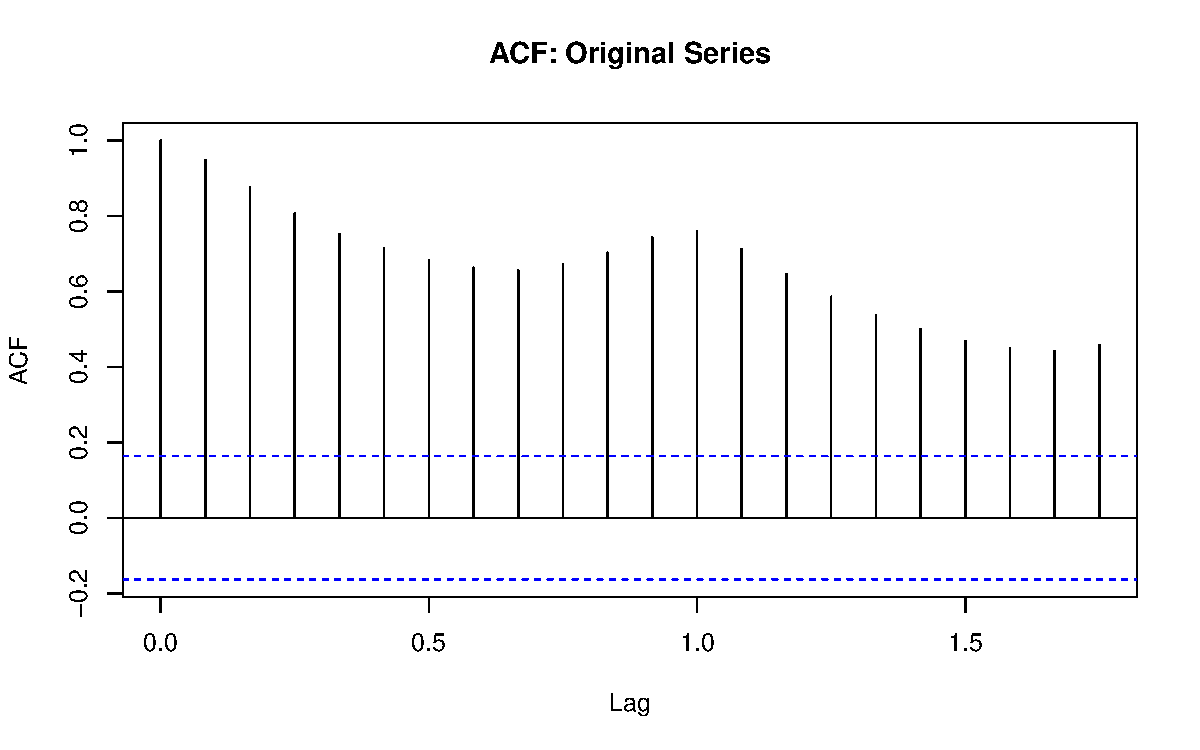
\includegraphics[keepaspectratio]{03-chap3_files/figure-pdf/unnamed-chunk-8-2.pdf}}

\begin{Shaded}
\begin{Highlighting}[]
\CommentTok{\# 2. First difference (remove trend)}
\NormalTok{diff1 }\OtherTok{\textless{}{-}} \FunctionTok{diff}\NormalTok{(ts\_data, }\AttributeTok{differences =} \DecValTok{1}\NormalTok{)}
\FunctionTok{plot}\NormalTok{(diff1, }\AttributeTok{main =} \StringTok{"1st Difference (Remove Trend)"}\NormalTok{, }\AttributeTok{ylab =} \StringTok{"Difference"}\NormalTok{)}
\end{Highlighting}
\end{Shaded}

\pandocbounded{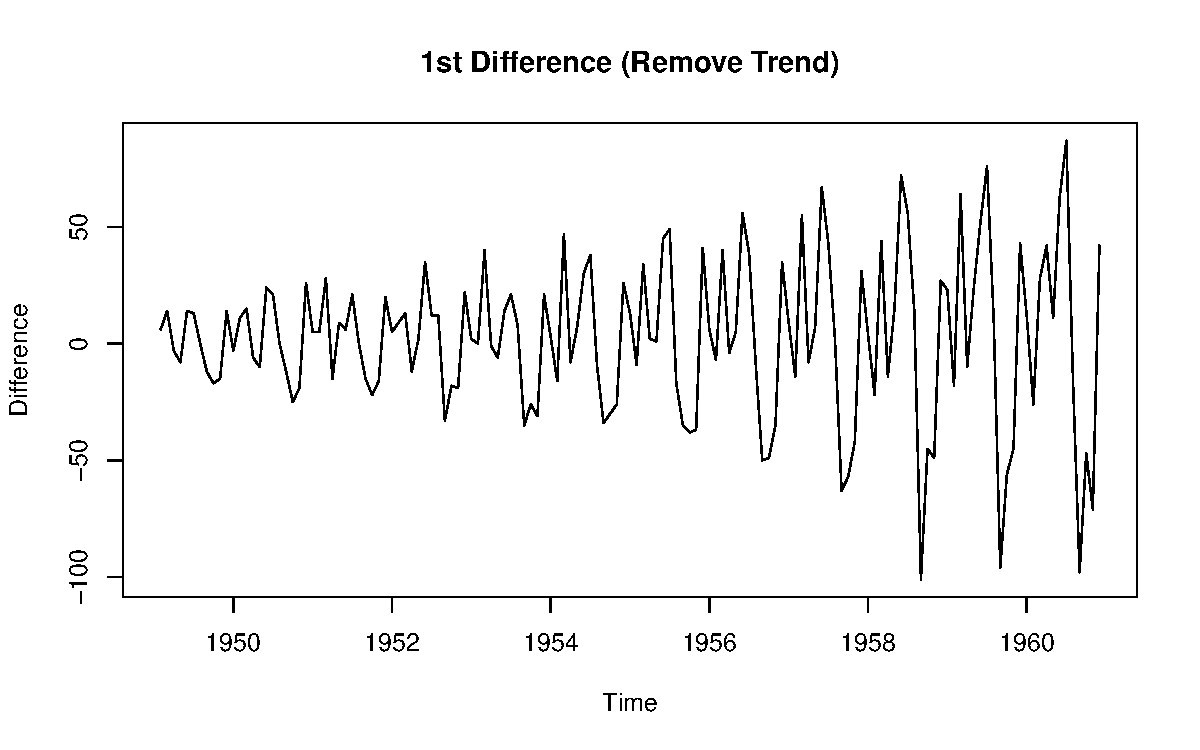
\includegraphics[keepaspectratio]{03-chap3_files/figure-pdf/unnamed-chunk-8-3.pdf}}

\begin{Shaded}
\begin{Highlighting}[]
\FunctionTok{acf}\NormalTok{(diff1, }\AttributeTok{main =} \StringTok{"ACF: 1st Difference"}\NormalTok{)}
\end{Highlighting}
\end{Shaded}

\pandocbounded{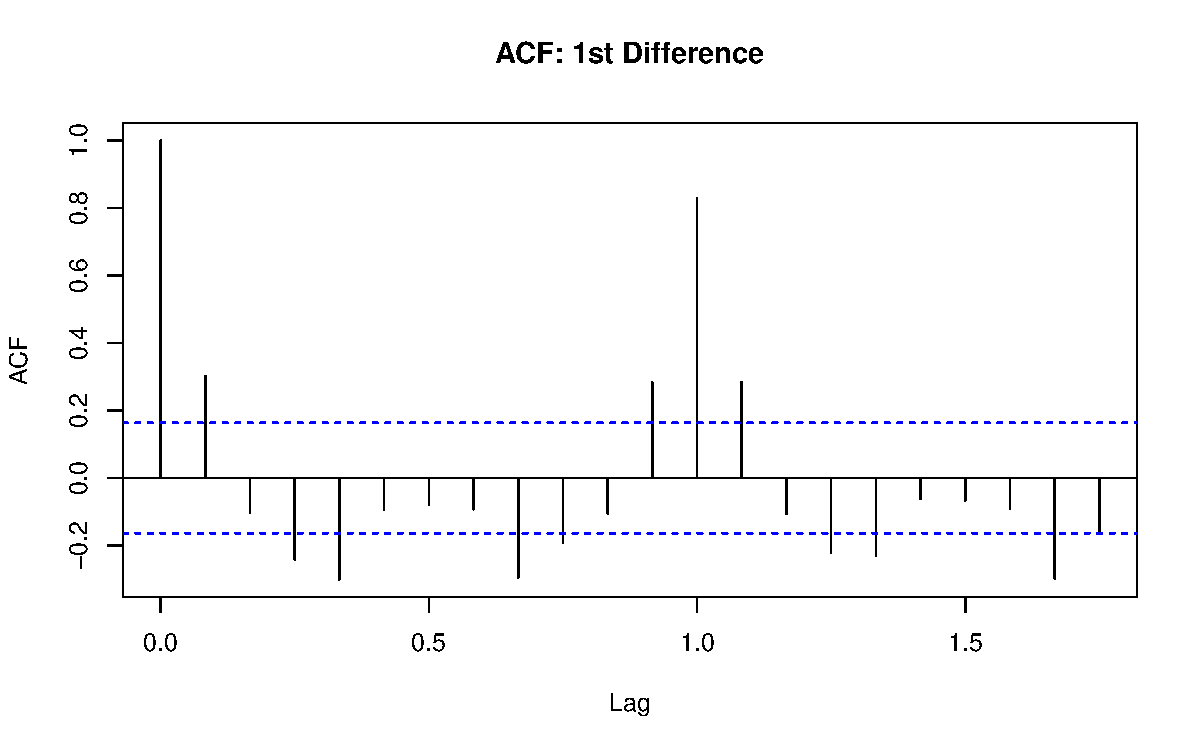
\includegraphics[keepaspectratio]{03-chap3_files/figure-pdf/unnamed-chunk-8-4.pdf}}

\begin{Shaded}
\begin{Highlighting}[]
\CommentTok{\# 3. Seasonal difference (lag = 12, remove seasonality)}
\NormalTok{diff\_seasonal }\OtherTok{\textless{}{-}} \FunctionTok{diff}\NormalTok{(diff1, }\AttributeTok{lag =} \DecValTok{12}\NormalTok{)}
\FunctionTok{plot}\NormalTok{(diff\_seasonal, }\AttributeTok{main =} \StringTok{"Seasonal Difference (Remove Seasonality)"}\NormalTok{, }\AttributeTok{ylab =} \StringTok{"Difference"}\NormalTok{)}
\end{Highlighting}
\end{Shaded}

\pandocbounded{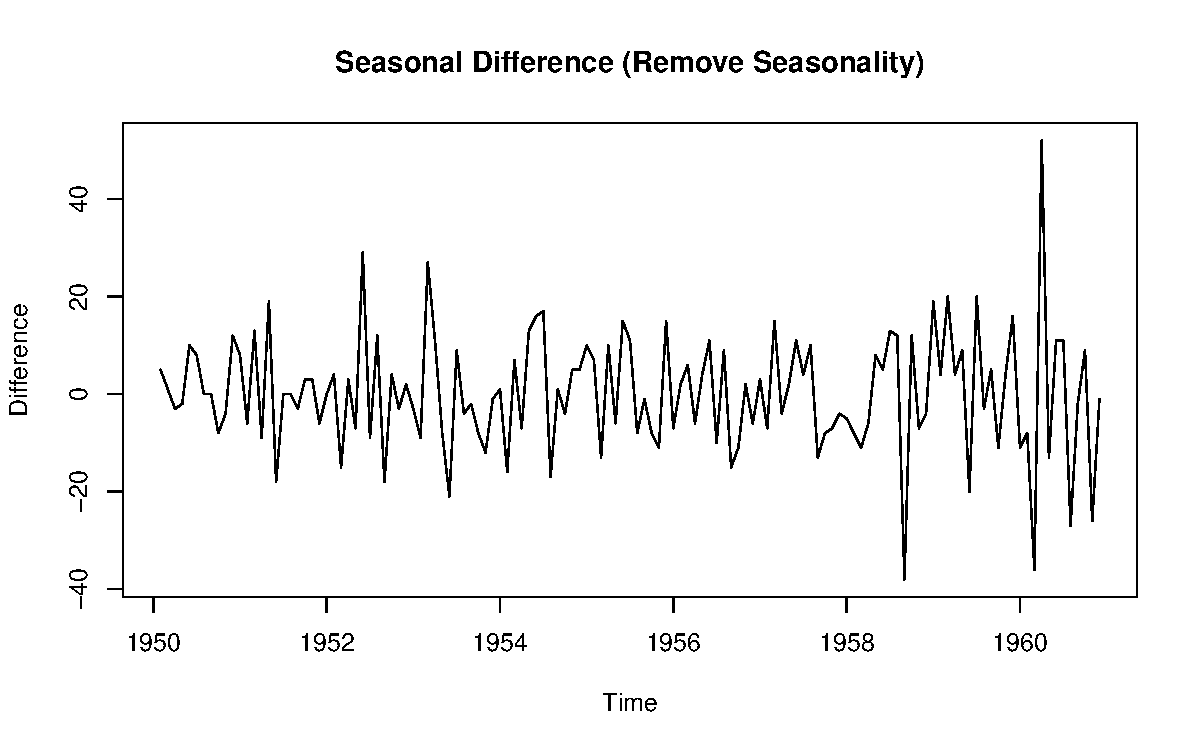
\includegraphics[keepaspectratio]{03-chap3_files/figure-pdf/unnamed-chunk-8-5.pdf}}

\begin{Shaded}
\begin{Highlighting}[]
\FunctionTok{acf}\NormalTok{(diff\_seasonal, }\AttributeTok{main =} \StringTok{"ACF: Seasonal Difference"}\NormalTok{)}
\end{Highlighting}
\end{Shaded}

\pandocbounded{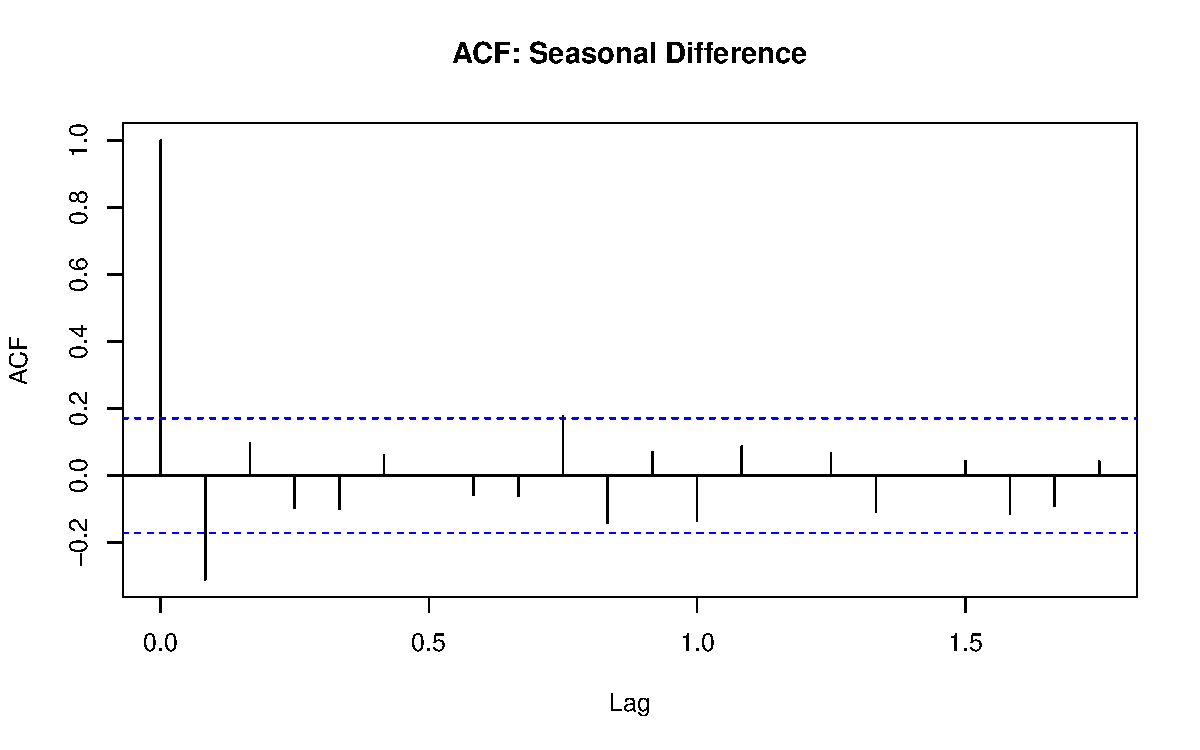
\includegraphics[keepaspectratio]{03-chap3_files/figure-pdf/unnamed-chunk-8-6.pdf}}

\begin{Shaded}
\begin{Highlighting}[]
\CommentTok{\# 3. Seasonal difference (lag = 12, remove seasonality from the original series)}
\NormalTok{diff\_seasonal\_only }\OtherTok{\textless{}{-}} \FunctionTok{diff}\NormalTok{(ts\_data, }\AttributeTok{lag =} \DecValTok{12}\NormalTok{)}
\FunctionTok{plot}\NormalTok{(diff\_seasonal\_only, }\AttributeTok{main =} \StringTok{"Seasonal Difference (Remove Seasonality)"}\NormalTok{, }\AttributeTok{ylab =} \StringTok{"Difference"}\NormalTok{)}
\end{Highlighting}
\end{Shaded}

\pandocbounded{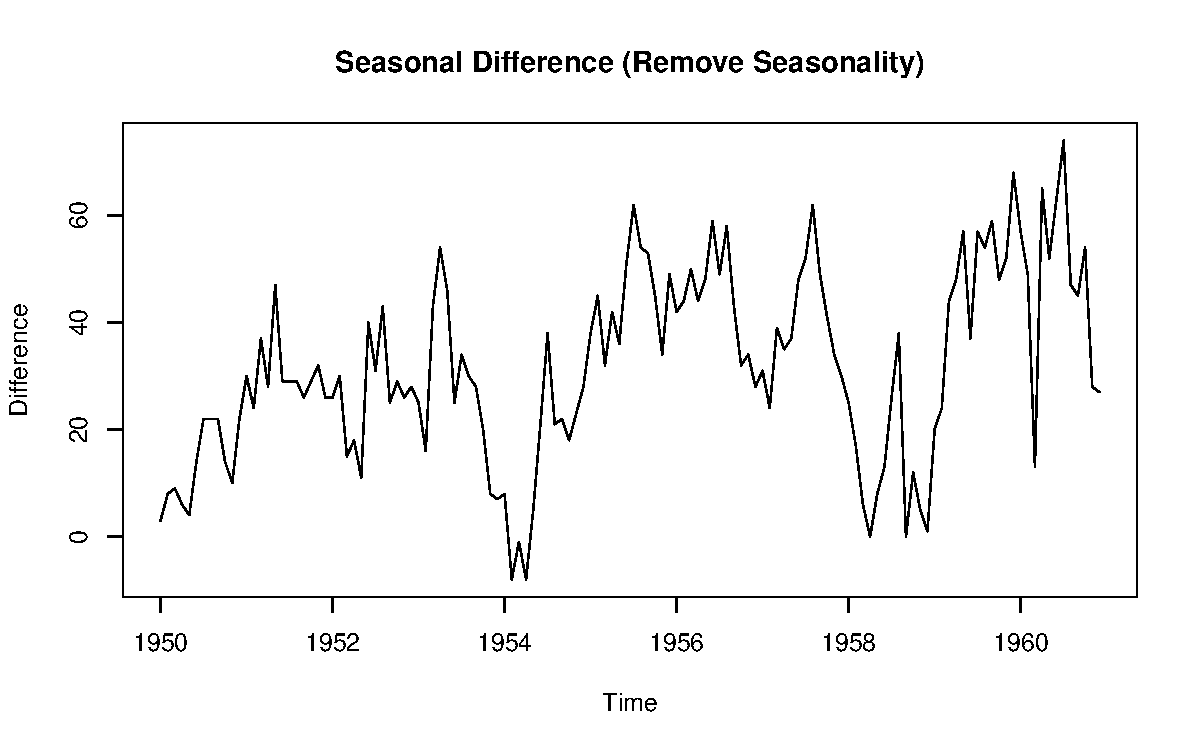
\includegraphics[keepaspectratio]{03-chap3_files/figure-pdf/unnamed-chunk-8-7.pdf}}

\begin{Shaded}
\begin{Highlighting}[]
\FunctionTok{acf}\NormalTok{(diff\_seasonal\_only, }\AttributeTok{main =} \StringTok{"ACF: Seasonal Difference"}\NormalTok{)}
\end{Highlighting}
\end{Shaded}

\pandocbounded{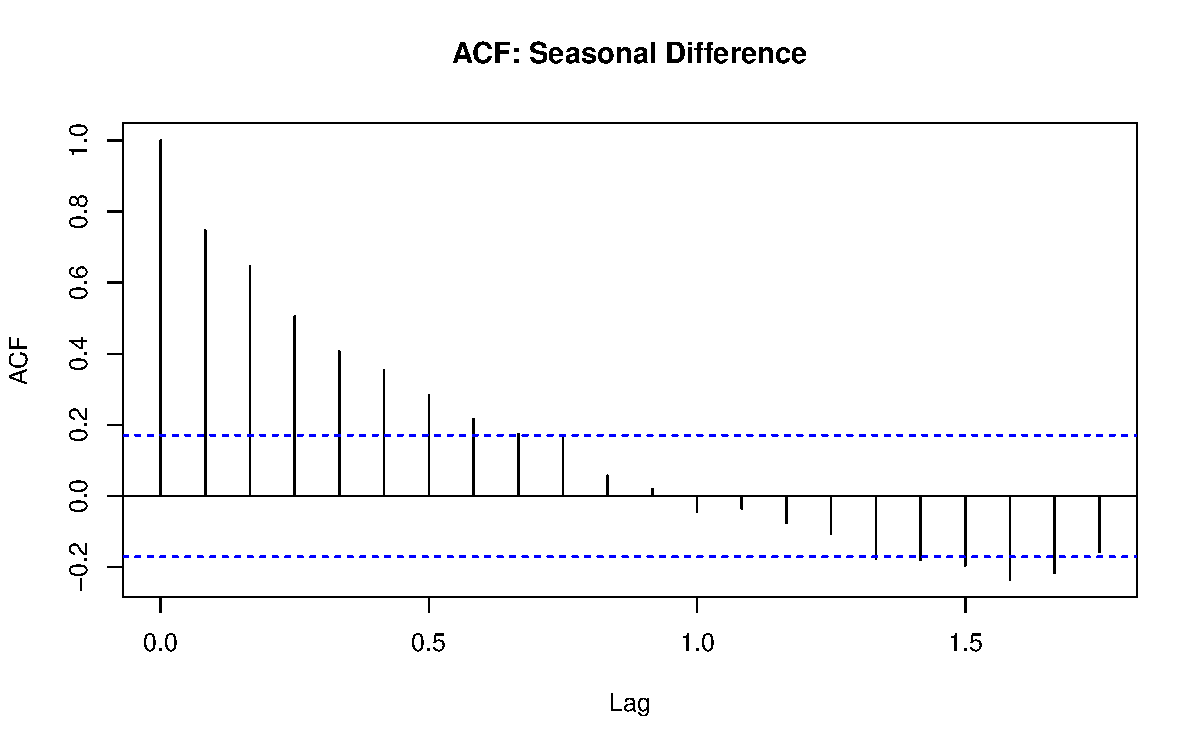
\includegraphics[keepaspectratio]{03-chap3_files/figure-pdf/unnamed-chunk-8-8.pdf}}

\begin{Shaded}
\begin{Highlighting}[]
\FunctionTok{head}\NormalTok{(ts\_data, }\DecValTok{14}\NormalTok{)}
\end{Highlighting}
\end{Shaded}

\begin{verbatim}
     Jan Feb Mar Apr May Jun Jul Aug Sep Oct Nov Dec
1949 112 118 132 129 121 135 148 148 136 119 104 118
1950 115 126                                        
\end{verbatim}

\begin{Shaded}
\begin{Highlighting}[]
\FunctionTok{head}\NormalTok{(diff1, }\DecValTok{14}\NormalTok{)}
\end{Highlighting}
\end{Shaded}

\begin{verbatim}
     Jan Feb Mar Apr May Jun Jul Aug Sep Oct Nov Dec
1949       6  14  -3  -8  14  13   0 -12 -17 -15  14
1950  -3  11  15                                    
\end{verbatim}

\begin{Shaded}
\begin{Highlighting}[]
\FunctionTok{head}\NormalTok{(diff\_seasonal, }\DecValTok{14}\NormalTok{)}
\end{Highlighting}
\end{Shaded}

\begin{verbatim}
     Jan Feb Mar Apr May Jun Jul Aug Sep Oct Nov Dec
1950       5   1  -3  -2  10   8   0   0  -8  -4  12
1951   8  -6  13                                    
\end{verbatim}

\begin{Shaded}
\begin{Highlighting}[]
\FunctionTok{head}\NormalTok{(diff\_seasonal\_only, }\DecValTok{14}\NormalTok{)}
\end{Highlighting}
\end{Shaded}

\begin{verbatim}
     Jan Feb Mar Apr May Jun Jul Aug Sep Oct Nov Dec
1950   3   8   9   6   4  14  22  22  22  14  10  22
1951  30  24                                        
\end{verbatim}

\section{Notation: I(d)}\label{notation-id}

Integrated to order \(d\): Series can be made stationary by differencing
\(d\) times.

\begin{itemize}
\tightlist
\item
  Known as \(I(d)\) process.
\end{itemize}

\textbf{Question:} Show that random walk process is an \(I(1)\) process.

The random walk process is called a unit root process. (If one of the
roots turns out to be one, then the process is called unit root
process.)

\section{Variance stabilization}\label{variance-stabilization}

Transform the series.

Eg:

\begin{itemize}
\item
  Square root: \(W_t = \sqrt{Y_t}\)
\item
  Logarithm: \(W_t = log({Y_t})\)

  \begin{itemize}
  \item
    This very useful.
  \item
    Interpretable: Changes in a log value are \textbf{relative (percent)
    changes on the original sclae}.
  \end{itemize}
\end{itemize}

\begin{Shaded}
\begin{Highlighting}[]
\NormalTok{log\_ts }\OtherTok{\textless{}{-}} \FunctionTok{log}\NormalTok{(ts\_data)}
\FunctionTok{plot}\NormalTok{(log\_ts, }\AttributeTok{main =} \StringTok{"Log{-}Transformed Series"}\NormalTok{, }\AttributeTok{ylab =} \StringTok{"log(Passengers)"}\NormalTok{, }\AttributeTok{col =} \StringTok{"steelblue"}\NormalTok{)}
\end{Highlighting}
\end{Shaded}

\pandocbounded{\includegraphics[keepaspectratio]{03-chap3_files/figure-pdf/unnamed-chunk-10-1.pdf}}

\bookmarksetup{startatroot}

\chapter{Models For Stationary Time
Series}\label{models-for-stationary-time-series}

In this chapter we will discuss family of autoregressive moving average
(ARMA) time series models.

\section{General Linear Process}\label{general-linear-process}

A \textbf{linear process} is a time series written as an infinite linear
combination of random shocks \(\{\varepsilon_t\}\). These shocks are
randomly drawn from a fixed distribution, usually Normal and having mean
zero and variance \(\sigma^2_{\epsilon}\). Such a sequence is called a
white noise process.

\[X_t = \mu + \sum_{j=0}^{\infty} \psi_j \, \varepsilon_{t-j},\]

or

\[X_t = \mu + \Psi(B)\epsilon_t\]

where,

\(\mu\) is a parameter that determines the ``level'' of the process

\(\{\psi_j\}\) are coefficients (weights)

\(\varepsilon_t \sim \text{i.i.d. } (0, \sigma^2_\epsilon)\) are white
noise shocks.

\(\Psi(B)\) is the linear operator that transforms \(\epsilon_t\) into
\(X_t\). This is called transfer function or linear filter.

\section{Moving Average Processes}\label{moving-average-processes}

If only finitely many coefficients \(\psi_j\) are nonzero, say up to lag
\(q\), then we have an MA(\(q\)) process:

\[X_t = \mu + \varepsilon_t + \theta_1 \varepsilon_{t-1} + \dots + \theta_q \varepsilon_{t-q},\]

where:

\begin{itemize}
\item
  \(\mu\) is the mean,
\item
  \(\varepsilon_t \sim \text{i.i.d. }(0, \sigma^2)\) are white noise
  shocks,
\item
  \(\theta_1, \dots, \theta_q\) are the MA coefficients.
\end{itemize}

So we can write:

\[\text{MA}(q) \subset \text{Linear Process}.\]

\section{Autoregressive Processes}\label{autoregressive-processes}

\(Y_t = \alpha + \phi_1 Y_{t-1} + \phi_2 Y_{t-2} + \dots + \phi_p Y_{t-p} + \epsilon_t\)

Where:

\(Y_t\) is the value at time \(t\)

\(\alpha\) is a constant,

\(\phi_1, \phi_2,...\phi_p\) are the parameters,

\(\epsilon_t\) is white noise (error term),

\(p\) is the order of the AR model.

\section{AR processes are also just special cases of the general linear
process}\label{ar-processes-are-also-just-special-cases-of-the-general-linear-process}

If the AR process is causal (i.e., roots of the characteristic
polynomial lie outside the unit circle), then it can be written as an
infinite linear process:

\[X_t = \sum_{j=0}^{\infty} \psi_j \, \varepsilon_{t-j},\]

where:

\begin{itemize}
\item
  \(\varepsilon_t \sim \text{i.i.d. }(0, \sigma^2)\) are white noise
  shocks,
\item
  \(\psi_j\) are coefficients determined from the AR parameters.
\end{itemize}

\subsection{AR(p) Process as an Infinite Linear Process Using Backshift
Operator}\label{arp-process-as-an-infinite-linear-process-using-backshift-operator}

Start with the AR(p) process:

\[X_t = \phi_1 X_{t-1} + \phi_2 X_{t-2} + \dots + \phi_p X_{t-p} + \varepsilon_t,\]

where \(\varepsilon_t \sim \text{i.i.d. }(0, \sigma^2)\) are white noise
shocks.

\subsubsection{1. Define the backshift operator
(B)}\label{define-the-backshift-operator-b}

\[B X_t = X_{t-1}, \quad B^2 X_t = X_{t-2}, \dots, B^p X_t = X_{t-p}.\]

\subsubsection{2. Rewrite the AR(p) process using
(B)}\label{rewrite-the-arp-process-using-b}

\[X_t - \phi_1 B X_t - \phi_2 B^2 X_t - \dots - \phi_p B^p X_t = \varepsilon_t\]

Factor out \(X_t\):

\[(1 - \phi_1 B - \phi_2 B^2 - \dots - \phi_p B^p) X_t = \varepsilon_t\]

Define the AR polynomial:

\[\phi(B) = 1 - \phi_1 B - \phi_2 B^2 - \dots - \phi_p B^p\]

Then the AR(p) process becomes:

\[\phi(B) X_t = \varepsilon_t\]

\subsubsection{3. Express as an infinite linear
process}\label{express-as-an-infinite-linear-process}

If the AR process is \textbf{causal} (roots of \(\phi(z)=0\) lie outside
the unit circle), we can invert the operator:

\[X_t = \phi(B)^{-1} \varepsilon_t\]

Expanding gives:

\[X_t = \sum_{j=0}^{\infty} \psi_j \, \varepsilon_{t-j},\]

where the coefficients \(\psi_j\) are determined recursively from the AR
parameters \(\phi_1, \dots, \phi_p\).

This shows that causal AR processes are \textbf{special cases of the
general linear process}.

\section{In-class: Properties of AR(1)
process}\label{in-class-properties-of-ar1-process}

Derive

\begin{itemize}
\item
  Mean
\item
  Variance
\item
  Covariance
\item
  Autocorrelation function of an AR(1) process
\end{itemize}

\section{In-class: Properties of AR(2)
process}\label{in-class-properties-of-ar2-process}

Derive

\begin{itemize}
\item
  Mean
\item
  Variance
\item
  Covariance
\item
  Autocorrelation function of an AR(1) process
\end{itemize}

\section{In-class: Properties of AR(P)
process}\label{in-class-properties-of-arp-process}

Derive

\begin{itemize}
\item
  Mean
\item
  Variance
\item
  Covariance
\item
  Autocorrelation function of an AR(P) process
\end{itemize}

\section{Properties of AR(1) model}\label{properties-of-ar1-model}

Consider the following \(AR(1)\) model.

\begin{equation}
Y_t=\phi_0+\phi_1Y_{t-1}+\epsilon_{t}
\end{equation}

where \({\epsilon_t}\) is assumed to be a white noise process with mean
zero and variance \(\sigma^2\).

\subsection{Mean}\label{mean}

Assuming that the series is weak stationary, we have \(E(Y_t)=\mu\),
\(Var(Y_t)=\gamma_0\), and \(Cov(Y_t, Y_{t-k})=\gamma_k\), where \(\mu\)
and \(\gamma_0\) are constants. Given that \({\epsilon_t}\) is a white
noise, we have \(E(\epsilon_t)=0\). The mean of \(AR(1)\) process can be
computed as follows:

\[
\begin{aligned}
  E(Y_t) &= E(\phi_0+\phi_1 Y_{t-1}) \\
         &= E(\phi_0) +E(\phi_1 Y_{t-1}) \\
         &= \phi_0 +\phi_1 E(Y_{t-1}). \\
\end{aligned}
\]

Under the stationarity condition, \(E(Y_t)=E(Y_{t-1})=\mu\). Thus we get

\[\mu = \phi_0+\phi_1\mu.\]

Solving for \(\mu\) yields

\begin{equation}
E(Y_t)=\mu=\frac{\phi_0}{1-\phi_1}.
\end{equation}

The results has two constraints for \(Y_t\). First, the mean of \(Y_t\)
exists if \(\phi_1 \neq 1 .\) The mean of \(Y_t\) is zero if and only if
\(\phi_0=0\).

\subsection{Variance and the stationary condition of AR (1)
process}\label{variance-and-the-stationary-condition-of-ar-1-process}

First take variance of both sides of Equation (1)

\[Var(Y_t)=Var(\phi_0+\phi_1 Y_{t-1}+\epsilon_t)\]

The \(Y_{t-1}\) occurred before time \(t\). The \(\epsilon_t\) does not
depend on any past observation. Hence, \(cov(Y_{t-1}, \epsilon_t)= 0\).
Furthermore, \({\epsilon_t}\) is a white noise. This gives

\[Var(Y_t)=\phi_1^2 Var(Y_{t-1})+\sigma^2.\]

Under the stationarity condition, \(Var(Y_t)=Var(Y_{t-1})\). Hence,

\[Var(Y_t)=\frac{\sigma^2}{1-\phi_1^2}.\]

provided that \(\phi_1^2 < 1\) or \(|\phi_1| < 1\) (The variance of a
random variable is bounded and non-negative). The necessary and
sufficient condition for the \(AR(1)\) model in Equation (1) to be
weakly stationary is \(|\phi_1| < 1\). This condition is equivalent to
saying that the root of \(1-\phi_1B = 0\) must lie outside the unit
circle. This can be explained as below

Using the backshift notation we can write \(AR(1)\) process as

\[Y_t = \phi_0 + \phi_1BY_{t} + \epsilon_t.\]

Then we get

\[(1-\phi_1B)Y_t=\phi_0 + \epsilon_t.\] The \(AR(1)\) process is said to
be stationary if the roots of \((1-\phi_1B)=0\) lie outside the unit
circle.

\subsection{Covariance}\label{covariance}

The covariance \(\gamma_k=Cov(Y_t, Y_{t-k})\) is called the lag-\(k\)
autocovariance of \(Y_t\). The two main properties of \(\gamma_k\): (a)
\(\gamma_0=Var(Y_t)\) and (b) \(\gamma_{-k}=\gamma_{k}\).

The lag-\(k\) autocovariance of \(Y_t\) is

\begin{equation}
\begin{aligned}
  \gamma_k &= Cov(Y_t, Y_{t-k}) \\
         &= E[(Y_t-\mu)(Y_{t-k}-\mu)] \\
         &= E[Y_tY_{t-k}-Y_t\mu-\mu Y_{t-k} +\mu^2] \\
         &= E(Y_t Y_{t-k}) - \mu^2. \\
\end{aligned}
\end{equation}

Now we have

\begin{equation}
  E(Y_t Y_{t-k}) = \gamma_k + \mu^2
\end{equation}

\subsection{Autocorrelation function of an AR(1)
process}\label{autocorrelation-function-of-an-ar1-process}

To derive autocorrelation function of an AR(1) process we first multiply
both sides of Equation (1) by \(Y_{t-k}\) and take expected values:

\[E(Y_tY_{t-k})=\phi_0E(Y_{t-k})+\phi_1 E(Y_{t-1}Y_{t-k})+E(\epsilon_tY_{t-k})\]
Since \(\epsilon_t\) and \(Y_{t-k}\) are independent and using the
results in Equation \textbf{?@eq-3}

\[\gamma_k + \mu^2 = \phi_0 \mu+\phi_1(\gamma_{k-1}+\mu^2)\]

Substituting the results in Equation (2) to Equation (3) we get

\begin{equation}
\gamma_k = \phi_1 \gamma_{k-1}.
\end{equation}

The autocorrelation function, \(\rho_k\), is defined as

\[\rho_k = \frac{\gamma_k}{\gamma_0}\].

Setting \(k=1\), we get \(\gamma_1 = \phi_1\gamma_0.\) Hence,

\[\rho_1=\phi_1.\]

Similarly with \(k=2\), \(\gamma_2 = \phi_1 \gamma_1\). Dividing both
sides by \(\gamma_0\) and substituting with \(\rho_1=\phi_1\) we get

\[\rho_2=\phi_1^2.\]

Now it is easy to see that in general

\begin{equation}
\rho_k = \frac{\gamma_k}{\gamma_0}=\phi_1^k 
\end{equation}

for \(k=0, 1, 2, 3, ...\).

Since \(|\phi_1| < 1,\) the autocorrelation function is an exponentially
decreasing as the number of lags \(k\) increases. There are two features
in the ACF of AR(1) process depending on the sign of \(\phi_1\). They
are,

\begin{enumerate}
\def\labelenumi{\arabic{enumi}.}
\item
  If \(0 < \phi_1 < 1,\) all correlations are positive.
\item
  if \(-1 < \phi_1 < 0,\) the lag 1 autocorrelation is negative
  (\(\rho_1=\phi_1\)) and the signs of successive autocorrelations
  alternate from positive to negative with their magnitudes decreasing
  exponentially.
\end{enumerate}

\section{Properties of AR(2) model}\label{properties-of-ar2-model}

Now consider a second-order autoregressive process (AR(2))

\begin{equation}
Y_t=\phi_0+\phi_1Y_{t-1}+\phi_2Y_{t-2}+\epsilon_t.
\end{equation}

\subsection{Mean}\label{mean-1}

\textbf{Question 1:} Using the same technique as that of the AR(1), show
that

\[E(Y_t) = \mu = \frac{\phi_0}{1-\phi_1 - \phi_2}\] and the mean of
\(Y_t\) exists if \(\phi_1 + \phi_2 \neq 1\).

\subsection{Variance}\label{variance}

\textbf{Question 2:} Show that
\[Var(Y_t) = \frac{(1-\phi_2)\sigma^2}{(1+\phi_2)((1+\phi_2)^2-\phi_1^2)}.\]

Here is a guide to the solution

Start with

\[Var(Y_t)=Var(\phi_0+\phi_1Y_{t-1}+\phi_2Y_{t-2}+\epsilon_t)\]

Solve it until you obtain the Eq. (a) as shown below.

\begin{equation}
\gamma_0 (1-\phi_1^2 - \phi_2^2) = 2\phi_1\phi_2\gamma_1+\sigma^2.
\end{equation}

Next multiply both sides of Equation 7 by \(Y_{t-1}\) and obtain an
expression for \(\gamma_1\). Let's call this Eq. (b).

Solve Eq. (a) and (b) for \(\gamma_0.\)

\subsection{Stationarity of AR(2)
process}\label{stationarity-of-ar2-process}

To discuss the stationarity condition of the \(AR(2)\) process we use
the roots of the characteristic polynomial. Here is the illustration.

Using the backshift notation we can write \(AR(2)\) process as

\[Y_t = \phi_0 + \phi_1 BY_{t} + \phi_2 B^2 Y_{t} + \epsilon_t.\]

Furthermore, we get

\[(1-\phi_1 B - \phi_2 B^2) Y_t = \phi_0 + \epsilon_t.\]

The \textbf{characteristic polynomial} of \(AR(2)\) process is

\[\Phi(B)=1-\phi_1 B - \phi_2 B^2.\]

and the corresponding \textbf{AR characteristic equation}

\[1-\phi_1 B - \phi_2 B^2=0.\]

For stationarity, the roots of AR characteristic equation must lie
outside the unit circle. The two roots of the AR characteristic equation
are

\[\frac{\phi_1 \pm \sqrt{\phi_1^2 + 4\phi_2}}{-2\phi_2}\]

Using algebraic manipulation, we can show that these roots will exceed 1
in modulus if and only if simultaneously \(\phi_1 + \phi_2 < 1,\)
\(\phi_2-\phi_1 < 1,\) and \(|\phi_2| < 1.\) This is called the
stationarity condition of \(AR(2)\) process.

\subsection{Autocorrelation function of an AR(2)
process}\label{autocorrelation-function-of-an-ar2-process}

To derive autocorrelation function of an AR(2) process we first multiply
both sides of Equation 7 by \(Y_{t-k}\) and take expected values:

\begin{align}
E(Y_tY_{t-k}) &= E(\phi_0Y_{t-k}+\theta_1Y_{t-1}Y_{t-k}+\theta_2Y_{t-2}Y_{t-k})+\epsilon_tY_{t-k} \\
&= \phi_0 E(Y_{t-k})+\phi_{1}E(Y_{t-1}Y_{t-k}) + \phi_2 E(Y_{t-2} Y_{t-k}) + E(\epsilon_tY_{t-k}).
\end{align}

Using the independence between \(\epsilon_t\) and \(Y_{t-1}\),
\(E(\epsilon_t Y_{t-k})=0\) and the results in Equation 4 (This is valid
for AR(2)) we have

\[\gamma_k + \mu^2 = \gamma_0 \mu + \theta_1 (\gamma_{k-1}+\mu^2)+\phi_2 (\gamma_{k-2}+\mu^2).\]

(Note that \(E(X_{t-1}X_{t-k})=E(X_{t-1}X_{(t-1)-(k-1)}=\gamma_{k-1})\))

Solving for \(\gamma_k\) we get

\begin{align}
 \gamma_k=\phi_1\gamma_{k-1}+\phi_2\gamma_{k-2}.
\end{align}

By dividing the both sides of Equation 10 by \(\gamma_0\), we have

\begin{align}
 \rho_k=\phi_1\rho_{k-1}+\phi_2\rho_{k-2}.
\end{align}

for \(k>0\).

Setting \(k=1\) and using \(\rho_0=1\) and \(\rho_{-1}=\rho_1\), we get
\textbf{the Yule-Walker equation for \(AR(2)\) process.}

\[\rho_1=\phi_1+\phi_2 \rho_1\] or

\[\rho_1 = \frac{\phi_1}{1-\phi_2}.\]

Similarly, we can show that

\[\rho_2 = \frac{\phi_2(1-\phi_2)+\phi_1^2}{(1-\phi_2)}.\]

\section{Properties of AR(p) model}\label{properties-of-arp-model}

The \(p\)th order autoregressive model can be written as

\begin{align}
Y_t = \phi_0 + \phi_1Y_{t-1}+\phi_2 Y_{t-2}+ ... + \phi_p Y_{t-p}+\epsilon_t.
\end{align}

The AR characteristic equation is

\[1-\phi_1B-\phi_2B^2-...-\phi_pB^p=0.\]

For stationarity of \(AR(p)\) process, the \(p\) roots of the AR
characteristic must lie outside the unit circle.

\subsection{Mean}\label{mean-2}

\textbf{Question 3: } Find \(E(Y_t)\) of \(AR(p)\) process.

\subsection{Variance}\label{variance-1}

\textbf{Question 4: } Find \(Var(Y_t)\) of \(AR(p)\) process.

\subsection{Autocorrelation function (ACF) of an AR(p)
process}\label{autocorrelation-function-acf-of-an-arp-process}

\textbf{Question 5: } Similar to the results in Equation 12 for
\(AR(2)\) process, obtain the following recursive relationship for
\(AR(p)\).

\begin{align}
\rho_k = \phi_1\rho_{k-1}+\phi_2 \rho_{k-2} + ... + \phi_p \rho_{k-p}.
\end{align}

Setting \(k=1, 2, ..., p\) into Equation 14 and using \(\rho_0=1\) and
\(\rho_{-k}=\rho_k\), we get the Yule-Walker equations for \(AR(p)\)
process

\begin{equation}
\begin{aligned}
  \rho_1 &= \phi_1+\phi_2 \rho_{1} + ... + \phi_p \rho_{p-1}\\
  \rho_2 &= \phi_1 \rho_1+\phi_2  + ... + \phi_p \rho_{p-2}\\
  ... \\
  \rho_p &= \phi_1 \rho_{p-1} +\phi_2 \rho_{p-2}  + ... + \phi_p \\
\end{aligned}
\end{equation}

The Yule-Walker equations in 14 can be written in matrix form as below.

\[\left[\begin{array}
{r}
\rho_1  \\
\rho_2  \\
.\\
.\\
.\\
\rho_p
\end{array}\right] = \left[\begin{array}
{rrrrrrr}
1 & \rho_1 & \rho_2 & .&.&.& \rho_{p-1} \\
\rho_1 & 1 & \rho_1 & .&.&.& \rho_{p-2} \\
. & . & . & .&.&.& . \\
. & . & . & .&.&.& . \\
. & . & . & .&.&.& . \\
\rho_{p-1} & \rho_{p-2} & \rho_{p-3} & .&.&.& 1 \\
\end{array}\right] \left[\begin{array}
{r}
\phi_1  \\
\phi_2  \\
.\\
.\\
.\\
\phi_p
\end{array}\right]
\]

or

\[\bm{\rho_p}=\bm{P_p\phi}.\]

where,

\[\bm{\rho_p} = \left[\begin{array}
{r}
\rho_1  \\
\rho_2  \\
.\\
.\\
.\\
\rho_p
\end{array}\right], \bm{P_p} = \left[\begin{array}
{rrrrrrr}
1 & \rho_1 & \rho_2 & .&.&.& \rho_{p-1} \\
\rho_1 & 1 & \rho_1 & .&.&.& \rho_{p-2} \\
. & . & . & .&.&.& . \\
. & . & . & .&.&.& . \\
. & . & . & .&.&.& . \\
\rho_{p-1} & \rho_{p-2} & \rho_{p-3} & .&.&.& 1 \\
\end{array}\right], \bm{\phi} = \left[\begin{array}
{r}
\phi_1  \\
\phi_2  \\
.\\
.\\
.\\
\phi_p
\end{array}\right]\]

The parameters can be estimated using

\[\bm{\phi}=\bm{P_p^{-1}\rho_p}.\]

\textbf{Question 6:} Obtain the parameters of an \(AR(3)\) process whose
first autocorrelations are \(\rho_1=0.9\); \(\rho_2=0.9\);
\(\rho_3=0.5\). Is the process stationary?

\section{The partial autocorrelation function
(PACF)}\label{the-partial-autocorrelation-function-pacf}

Let \(\phi_{ki}\), the \(j\)th coefficient in an \(AR(k)\) model. Then,
\(\phi_{kk}\) is the last coefficient. From Equation
\textbf{?@eq-yulep}, the \(\phi_{kj}\) satisfy the set of equations

\begin{equation}
\rho_j=\phi_{k1}\rho_{j-1}+...+\phi_{k(k-1)}\rho_{j-k+1}+\phi_{kk}\rho_{j-k},
\end{equation}

for \(j=1, 2, ...k\), leading to the Yule-Walker equations which may be
written

\begin{equation}
\left[\begin{array}
{r}
\rho_1  \\
\rho_2  \\
.\\
.\\
.\\
\rho_k
\end{array}\right] = \left[\begin{array}
{rrrrrrr}
1 & \rho_1 & \rho_2 & .&.&.& \rho_{k-1} \\
\rho_1 & 1 & \rho_1 & .&.&.& \rho_{k-2} \\
. & . & . & .&.&.& . \\
. & . & . & .&.&.& . \\
. & . & . & .&.&.& . \\
\rho_{k-1} & \rho_{k-2} & \rho_{k-3} & .&.&.& 1 \\
\end{array}\right] \left[\begin{array}
{r}
\phi_{k1}  \\
\phi_{k2}  \\
.\\
.\\
.\\
\phi_{kk}
\end{array}\right]
\end{equation}

or

\[\bm{\rho_k}=\bm{P_k\phi_k}.\]

where

\[\bm{\rho_k} = \left[\begin{array}
{r}
\rho_1  \\
\rho_2  \\
.\\
.\\
.\\
\rho_k
\end{array}\right], \bm{P_k} =\left[\begin{array}
{rrrrrrr}
1 & \rho_1 & \rho_2 & .&.&.& \rho_{k-1} \\
\rho_1 & 1 & \rho_1 & .&.&.& \rho_{k-2} \\
. & . & . & .&.&.& . \\
. & . & . & .&.&.& . \\
. & . & . & .&.&.& . \\
\rho_{k-1} & \rho_{k-2} & \rho_{k-3} & .&.&.& 1 \\
\end{array}\right], \bm{\phi_k} = \left[\begin{array}
{r}
\phi_{k1}  \\
\phi_{k2}  \\
.\\
.\\
.\\
\phi_{kk}
\end{array}\right]\]

For each \(k\), we compute the coefficients \(\phi_{kk}\). Solving the
equations for \(k=1, 2, 3...\) successively, we obtain

For \(k=1\),

\begin{equation}
\phi_{11}=\rho_1.
\end{equation}

For \(k=2\),

\begin{equation}
\phi_{22}=\frac{\left[\begin{array}
{rr}
1 & \rho_2  \\
\rho_1 & \rho_2  \\
\end{array}\right]}{\left[\begin{array}
{rr}
1 & \rho_1  \\
\rho_1 & 1  \\
\end{array}\right]} = \frac{\rho_2-\rho_1^2}{1-\rho_1^2}
\end{equation}

For \(k=3\),

\begin{equation}
\phi_{33}=\frac{\left[\begin{array}
{rrr}
1 & \rho_1 & \rho_1  \\
\rho_1 & 1 & \rho_2  \\
\rho_2 & \rho_1 & \rho_3  \\
\end{array}\right]}{\left[\begin{array}
{rrr}
1 & \rho_1 & \rho_2  \\
\rho_1 & 1 & \rho_1  \\
\rho_2 & \rho_1 & 1  \\
\end{array}\right]}
\end{equation}

The quantity \(\phi_{kk}\) is called the partial autocorrelation at lag
\(k\) and can be defined as
\[\phi_{kk}=Corr(Y_tY_{t-k}|Y_{t-1}, Y_{t-2},..., Y_{t-k+1}).\] The
partial autocorrelation between \(Y_t\) and \(Y_{t-k}\) is the
correlation between \(Y_t\) and \(Y_{t-k}\) after removing the effect of
the intermediate variables \(Y_{t-1}, Y_{t-2}, ..., Y_{t-k+1}\).

In general the determinant in the numerator of Equations 18, 19 and 20
has the same elements as that in the denominator, but replacing the last
column with \(\bm{\rho_k}= (\rho_1, \rho_2,...\rho_k).\)

\subsection{PACF for AR(1) models}\label{pacf-for-ar1-models}

From Equation 6 we have

\(\rho_k=\phi_1^k\) for \(k=0, 1, 2, 3,...\)

Hence, for \(k=1\), the first partial autocorrelation coefficient is

\[\phi_{11}=\rho_1=\phi_1.\] From 19 for \(k=2\), the second partial
autocorrelation coefficient is

\[\phi_{22}=\frac{\rho_2-\rho_1^2}{1-\rho_1^2}=\frac{\phi_1^2-\phi_1^2}{1-\phi_1^2} = 0\].

Similarly, for \(AR(1)\) we can show that \(\phi_{kk}=0\) for all
\(k > 0\). Hence, for \(AR(1)\) process the partial autocorrelation is
non-zero for lag \(1\) which is the order of the process, but is zero
for lags beyond the order 1.

\subsection{PACF for AR(2) model}\label{pacf-for-ar2-model}

\textbf{Question 7:} For \(AR(2)\) process show that \(\phi_{kk}=0\) for
all \(k>2\). Sketch the PACF of \(AR(2)\) process.

\subsection{PACF for AR(P) model}\label{pacf-for-arp-model}

In general for \(AR(p)\) precess, the partial autocorrelation function
\(\phi_{kk}\) is non-zero for \(k\) less than or equal to \(p\) (the
order of the process) and zero for all \(k\) greater than \(p\). In
other words, the partial autocorrelation function of a \(AR(p)\) process
has a cut-off after lag \(p\).

\section{Moving average (MA) models}\label{moving-average-ma-models}

We first derive the properties of \(MA(1)\) and \(MA(2)\) models and
then give the results for the general \(MA(q)\) model.

\section{Properties of MA(1) model}\label{properties-of-ma1-model}

The general form for \(MA(1)\) model is

\begin{equation}
Y_t = \theta_0 + \theta_1 \epsilon_{t-1} + \epsilon_t
\end{equation}

where \(\theta_0\) is a constant and \({\epsilon_t}\) is a white noise
series.

\subsection{Mean}\label{mean-3}

\textbf{Question 8:} Show that \(E(Y_t) = \theta_0\).

\subsection{Variance}\label{variance-2}

\textbf{Question 9:} Show that \(Var(Y_t) = (1+\theta_1^2)\sigma^2\).

We can see both mean and variance are time-invariant. \(MA\) models are
finite linear combinations of a white noise sequence. Hence, \(MA\)
processes are always weakly stationary.

\subsection{Autocorrelation function of an MA(1)
process}\label{autocorrelation-function-of-an-ma1-process}

\subsubsection{Method 1}\label{method-1}

To obtain the autocorrelation function of \(MA(1)\), we first multiply
both sides of Equation 21 by \(Y_{t-k}\) and take the expectation.

\begin{equation}
\begin{aligned}
E[Y_tY_{t-k}] &= E[\theta_0 Y_{t-k} + \theta_1 \epsilon_{t-1} Y_{t-k} + \epsilon_t Y_{t-k}]\\
&= \theta_0 E(Y_{t-k}) + \theta_1 E(\epsilon_{t-1}Y_{t-k}) + E(\epsilon_t Y_{t-k})\\
\end{aligned}
\end{equation}

Using the independence between \(\epsilon_t\) and \(Y_{t-k}\) (future
error and past observation) \(E(\epsilon_t Y_{t-k}) = 0\). Now we have

\begin{equation}
E[Y_tY_{t-k}] = \theta_0^2  + \theta_1 E(\epsilon_{t-1}Y_{t-k}) 
\end{equation}

Now let's obtain an expression for \(E[Y_t Y_{t-k}]\).

\begin{equation}
\begin{aligned}
  \gamma_k &= Cov(Y_t, Y_{t-k}) \\
         &= E[(Y_t-\theta_0)(Y_{t-k}-\theta_0)] \\
         &= E[Y_tY_{t-k}-Y_t\theta_0-\theta_0 Y_{t-k} +\theta_0^2] \\
         &= E(Y_t Y_{t-k}) - \theta_0^2. \\
\end{aligned}
\end{equation}

Now we have

\begin{equation}
  E(Y_t Y_{t-k}) = \gamma_k + \theta_0^2.
\end{equation}

Using the Equations 23 and 25 we have

\begin{equation}
  \gamma_k = \theta_0^2 - \theta_0^2 + \theta_1E(\epsilon_{t-1}Y_{t-k}).
\end{equation}

Now let's consider the case \(k=1\).

\begin{equation}
  \gamma_1 = \theta_0^2 - \theta_0^2 + \theta_1E(\epsilon_{t-1}Y_{t-1})
\end{equation}

Today's error and today's value are dependent. Hence,
\(E(\epsilon_{t-1}Y_{t-1}) \neq 0.\) We first need to identify
\(E(\epsilon_{t-1}Y_{t-1})\).

\begin{equation}
\begin{aligned}
E(\epsilon_{t-1}Y_{t-1}) &= E(\theta_0 \epsilon_{t-1} + \theta_1 \epsilon_{t-2} \epsilon_{t-1}+ \epsilon_{t-1}^2)\\
\end{aligned}
\end{equation}

Since, \{\(\epsilon_t\)\} is a white noise process
\(E(\epsilon_{t-1}) = 0\) and \(E(\epsilon_{t-2} \epsilon_{t-1}) = 0\).
Hence, we have

\begin{equation}
\begin{aligned}
E(\epsilon_{t-1}Y_{t-1}) &= E(\epsilon_{t-1}^2)=\sigma^2\\
\end{aligned}
\end{equation}

Substituting 29 in 27 we get

\[\gamma_1=\theta_1\sigma^2\].

Furthermore, \(\gamma_0 = Var(Y_t)=  (1+\theta_1^2)\sigma^2\). Hence

\[\rho_1=\frac{\gamma_1}{\gamma_0}=\frac{\theta}{1+\theta_1^2}.\]

When \(k=2\), from Equation 27 and \(E(\epsilon_{t-1}Y_{k-2}) = 0\)
(future error and past observation) we get \(\gamma_2=0\). Hence
\(\rho_2=0\). Similarly, we can show that

\[\gamma_k = \rho_k=0\] for all \(k \geq 2\).

We can see that the ACF of \(MA(1)\) process is zero, beyond the order
of 1 of the process.

\subsubsection{Method 2: By using the definition of
covariance}\label{method-2-by-using-the-definition-of-covariance}

\begin{equation}
\begin{aligned}
\gamma_1 = Cov(Y_t, Y_{t-1}) &= Cov(\epsilon_t + \theta_1 \epsilon_{t-1}+ \theta_0, \epsilon_{t-1}+\theta_1 \epsilon_{t-2} + \theta_0)\\
&=Cov(\theta_1 \epsilon_{t-1}, \epsilon_{t-1})\\
&=\theta_1 \sigma^2.
\end{aligned}
\end{equation}

\begin{equation}
\begin{aligned}
\gamma_2=Cov(Y_t, Y_{t-2}) &= Cov(\epsilon_t + \theta_1 \epsilon_{t-1}+ \theta_0, \epsilon_{t-2}+\theta_1 \epsilon_{t-3} + \theta_0)\\
&=0.
\end{aligned}
\end{equation}

We have \(\gamma_0=\sigma^2(1+\theta_1^2)\), (Using the variance).

Hence

\[\rho_1=\frac{\gamma_1}{\gamma_0}=\frac{\theta_1}{1+\theta_1^2}.\]

Similarly we can show \(\gamma_k=\rho_k=0\) for all \(k \geq 2\).

\section{Properties of MA(2) model}\label{properties-of-ma2-model}

An \(MA(2)\) model is in the form

\begin{equation}
Y_t = \theta_0 + \theta_1 \epsilon_{t-1} + \theta_2 \epsilon_{t-2} + \epsilon_t
\end{equation}

where \(\theta_0\) is a constant and \({\epsilon_t}\) is a white noise
series.

\subsection{Mean}\label{mean-4}

\textbf{Question 10: } Show that \(E(Y_t) = \theta_0.\)

\subsection{Variance}\label{variance-3}

\textbf{Question 11: } Show that
\(Var(Y_t) = \sigma^2 (1+\theta_1^2 + \theta_2^2).\)

\subsection{Autocorrelation function of an MA(2)
process}\label{autocorrelation-function-of-an-ma2-process}

\textbf{Question 12: }For \(MA(2)\) process show that,

\[\rho_1=\frac{\theta_1(1+\theta_2)}{1+\theta_1^2+\theta_2^2},\]
\[\rho_2 = \frac{\theta_2}{1+\theta_1^2 + \theta_2^2},\]

and \(\rho_k=0\) for all \(k \geq 3.\)

\section{Properties of MA(q) model}\label{properties-of-maq-model}

\begin{equation}
Y_t = \theta_0 + \theta_1 \epsilon_{t-1} + \theta_2 \epsilon_{t-2} +...+ \theta_q \epsilon_{t-q} +\epsilon_t
\end{equation}

where \(\theta_0\) is a constant and \({\epsilon_t}\) is a white noise
series.

\subsection{Mean}\label{mean-5}

\textbf{Question 13:} Show that the constant term of an \(MA\) model is
the mean of the series (i.e.~\(E(Y_t)=\theta_0\)).

\subsection{Variance}\label{variance-4}

\textbf{Question 14:} Show that the variance of an \(MA\) model is
\[Var(Y_t)=(1+\theta_1^2+\theta_2^2+...+\theta_q^2)\sigma^2.\]

\subsection{Autocorrelation function of an MA(q)
process}\label{autocorrelation-function-of-an-maq-process}

\textbf{Question 15:} Show that the autocorrelation function of a
\(MA(q)\) process is zero, beyond the order of \(q\) of the process. In
other words, the autocorrelation function of a moving average process
has a cutoff after lag \(q\).

\section{Partial autocorrelation function of an MA(q)
process}\label{partial-autocorrelation-function-of-an-maq-process}

The partial autocorrelation functions for \(MA(q)\) models behave very
much like the autocorrelation functions of \(AR(p)\) models. The PACF of
\(MA\) models decays exponentially to zero, rather like ACF for \(AR\)
model.

\section{Dual relation between AR and MA
process}\label{dual-relation-between-ar-and-ma-process}

\textbf{Dual relation 1}

\textbf{First we consider the relation AR(p) \textless--\textgreater{}
MA(}\(\infty\)\textbf{)}

Let \(AR(p)\) be a \textbf{stationary} \(AR\) model with order \(p\).
Then,

\[Y_t = \phi_1Y_{t-1}+ \phi_2Y_{t-2}+...+ \phi_pY_{t-p}+\epsilon_t,\]
where \(\epsilon_t \sim WN(0, \sigma^2).\)

Using the backshift operator we can write the \(AR(p)\) model as

\[(1-\phi_1B-\phi_2B^2-...-\phi_pB^P)Y_t=\epsilon_t.\] Then

\[\phi(B)Y_t=\epsilon_t,\] where
\(\phi(B)=1-\phi_1B-\phi_2B^2-...-\phi_pB^p.\) Furthermore, \(Y_t\) can
be written as infinite sum of previous \(\epsilon\)'s as below

\[Y_t = \phi^{-1}(B)\epsilon_t,\] where \(\phi(B)\psi(B)=1\) and
\(\psi(B)=1+\Psi_1B+\psi_2B^2+...\) Then \[Y_t=\psi(B)\epsilon_t.\] This
is a representation of \(MA(\infty)\) process.

\textbf{Next, we consider the relation MA(q) \textless--\textgreater{}
AR(}\(\infty\)\textbf{)}

Let \(MA(q)\) be \textbf{invertible} moving average process

\[Y_t = \epsilon_t + \theta_t\epsilon_{t-1}+\theta_2\epsilon_{t-2}+...+\theta_p\epsilon_{t-q}.\]

Using the backshift operator we can write the \(MA(q)\) process as

\[Y_t = (1+\theta_1B+\theta_2B^2-...+\theta_qB^q)\epsilon_t.\]

Then,

\[Y_t = \theta(B)\epsilon_t,\]

where \(\theta(B)=1+\theta_1B+\theta_2B^2+...+\theta_1B^q.\) Hence, for
an \textbf{invertible} moving average process, \(Y_t\) can be
represented as a finite weighted sum of previous error terms,
\(\epsilon\). Furthermore, since the process is invertible
\(\epsilon_t\) can be represented as an infinite weighted sum of
previous \(Y\)'s as below

\[\epsilon_t=\theta^{-1}(B)Y_t,\] where \(\pi(B)\theta(B)=1\), and
\(\pi(B) = 1+\pi_1B+\pi B^2+...\). Hence,

\[\epsilon_t = \pi(B)Y_t.\] This is an representation of a
\(AR(\infty)\) process.

\textbf{Dual relation 2}

An \(MA(q)\) process has an ACF function that is zero beyond lag \(q\)
and its PACF is decays exponentially to 0. Consequently, an \(AR(p)\)
process has an PACF that is zero beyond lag-\(p\), but its ACF decays
exponentially to 0.

\textbf{Dual relation 3}

For an \(AR(p)\) process the roots of \(\phi(B)=0\) must lie outside the
unit circle to satisfy the condition of stationarity. However, the
parameters of the \(AR(p)\) are not required to satisfy any conditions
to ensure invertibility. Conversely, the parameters of the \(MA\)
process are not required to satisfy any condition to ensure
stationarity. However, to ensure the condition of invertibility, the
roots of \(\theta(B)=0\) must lie outside the unit circle.

\section{Autoregressive and Moving-average (ARMA)
models}\label{autoregressive-and-moving-average-arma-models}

current value = linear combination of past values + linear combination
of past error + current error

The \(ARMA(p, q)\) can be written as

\[Y_t=c+\phi_1 Y_{t-1}+\phi_2 Y_{t-2}+...+\phi_p Y_{t-p}+\theta_1\epsilon_{t-1}+\theta_2\epsilon_{t-2}+...+\theta_q\epsilon_{t-q}+\epsilon_t,\]
where \(\{\epsilon_t\}\) is a white noise process.

Using the back shift operator

\[\phi(B)Y_t=\theta(B)\epsilon_t,\] where \(\phi(.)\) and \(\theta(.)\)
are the \(p\)th and \(q\)th degree polynomials,

\[\phi(B)=1-\phi_1 \epsilon -...-\phi_p \epsilon^p,\] and
\[\theta(B)=1+\theta_1\epsilon+...+\theta_q\epsilon^q.\]

\section{Stationary condition}\label{stationary-condition}

Roots of \[\phi(B)=0\] lie outside the unit circle.

\section{Invertible condition}\label{invertible-condition}

Roots of \[\theta(B)=0\] lie outside the unit circle.

\section{Autocorrelation function and Partial autocorrelation
function}\label{autocorrelation-function-and-partial-autocorrelation-function}

The ACF of an ARMA model exhibits a pattern similar to that of an AR
model. The PACF of ARMA process behaves like the PACF of a MA process.
Hence, the ACF and PACF are not informative in determining the order of
an ARMA model.

\section{Theoretical ACF and PACF for AR, MA and ARMA
models}\label{theoretical-acf-and-pacf-for-ar-ma-and-arma-models}

Theoretical autocorrelation coefficients for some of the more common AR,
MA and ARMA models are shown here. However, the ACF and PACF calculated
from the data will not exactly match any set of theoretical ACF and PACF
because the ACF and PACF calculated from the data are subject to
sampling variation.

\href{https://www.xycoon.com/ar2_process.htm}{Reading}

\begin{longtable}[]{@{}
  >{\raggedright\arraybackslash}p{(\linewidth - 4\tabcolsep) * \real{0.1304}}
  >{\raggedright\arraybackslash}p{(\linewidth - 4\tabcolsep) * \real{0.4239}}
  >{\raggedright\arraybackslash}p{(\linewidth - 4\tabcolsep) * \real{0.4457}}@{}}
\toprule\noalign{}
\begin{minipage}[b]{\linewidth}\raggedright
Model
\end{minipage} & \begin{minipage}[b]{\linewidth}\raggedright
ACF Pattern
\end{minipage} & \begin{minipage}[b]{\linewidth}\raggedright
PACF Pattern
\end{minipage} \\
\midrule\noalign{}
\endhead
\bottomrule\noalign{}
\endlastfoot
\textbf{AR(p)} & Tails off gradually (decays) & Cuts off after lag
\emph{p} \\
\textbf{MA(q)} & Cuts off after lag \emph{q} & Tails off gradually
(decays) \\
\textbf{ARMA(p,q)} & Tails off gradually & Tails off gradually \\
\end{longtable}

Pure AR(p): Identifiable because PACF cuts off at lag p.

Pure MA(q): Identifiable because ACF cuts off at lag q.

ARMA(p,q): ❌ Not directly identifiable from ACF/PACF alone, because
both ACF and PACF tail off gradually.

\textbf{Why?}

AR and MA leave distinct signatures (one tails off, the other cuts off).

But when you mix them (ARMA), the cutoff disappears in both ACF and PACF
→ they both look like ``tails.''

So, with ARMA you cannot read off the orders (p, q) just by eyeballing
ACF/PACF. Instead:

Use ACF/PACF to guess a reasonable starting model (e.g., looks AR-like →
include AR part, looks MA-like → include MA part).

Then refine by fitting candidate ARMA models and comparing AIC/BIC (or
likelihood-based tests).

\textbf{Rule of thumb}

\begin{itemize}
\item
  If ACF shows a sharp cutoff but PACF tails → suspect MA.
\item
  If PACF shows a sharp cutoff but ACF tails → suspect AR.
\item
  If both tail → likely ARMA (but exact p,q needs model selection).
\end{itemize}

So in an ARMA, both ACF and PACF tail off, \textbf{but}:

\begin{itemize}
\item
  If the first few lags of the ACF are strong, it suggests an MA part.
\item
  If the first few lags of the PACF are strong, it suggests an AR part.
\end{itemize}

\section{ACF and PACF calculated from
data}\label{acf-and-pacf-calculated-from-data}

\begin{figure}[H]

{\centering \pandocbounded{\includegraphics[keepaspectratio]{04-chap4_files/figure-pdf/unnamed-chunk-1-1.pdf}}

}

\caption{ACF and PACF of AR(1), MA(1) and ARMA(1, 1) models calculated
from the data}

\end{figure}%

\section{References}\label{references}

Box, G. E., Jenkins, G. M., Reinsel, G. C., \& Ljung, G. M. (2015). Time
series analysis: forecasting and control.

\bookmarksetup{startatroot}

\chapter{Models for Nonstationary Series}\label{sec-ch5}

\section{Types of Nonstationarity and
Remedies}\label{types-of-nonstationarity-and-remedies}

\subsection{1. Deterministic trend}\label{deterministic-trend-1}

\begin{itemize}
\item
  A \textbf{deterministic trend} is a predictable, non-random component
  such as a straight line or quadratic curve.\\
  Example:

  \[X_t = \alpha + \beta t + \epsilon_t\]

  where \(\epsilon_t\) is stationary white noise.
\item
  Solution:

  \begin{itemize}
  \tightlist
  \item
    Fit and remove the trend (regression detrending), or\\
  \item
    Use first differencing (removes linear trend).\\
  \end{itemize}
\item
  After detrending, the residuals should be stationary.
\end{itemize}

\begin{Shaded}
\begin{Highlighting}[]
\FunctionTok{library}\NormalTok{(ggplot2)}
\FunctionTok{set.seed}\NormalTok{(}\DecValTok{123}\NormalTok{)}

\CommentTok{\# Parameters}
\NormalTok{n }\OtherTok{\textless{}{-}} \DecValTok{100}
\NormalTok{alpha }\OtherTok{\textless{}{-}} \DecValTok{10}
\NormalTok{beta }\OtherTok{\textless{}{-}} \FloatTok{0.5}

\CommentTok{\# Simulate deterministic trend with noise}
\NormalTok{t }\OtherTok{\textless{}{-}} \DecValTok{1}\SpecialCharTok{:}\NormalTok{n}
\NormalTok{epsilon }\OtherTok{\textless{}{-}} \FunctionTok{rnorm}\NormalTok{(n, }\AttributeTok{mean =} \DecValTok{0}\NormalTok{, }\AttributeTok{sd =} \DecValTok{1}\NormalTok{)}
\NormalTok{X }\OtherTok{\textless{}{-}}\NormalTok{ alpha }\SpecialCharTok{+}\NormalTok{ beta }\SpecialCharTok{*}\NormalTok{ t }\SpecialCharTok{+}\NormalTok{ epsilon}
\NormalTok{data }\OtherTok{\textless{}{-}} \FunctionTok{data.frame}\NormalTok{(t, X)}

\CommentTok{\# Fit regression for detrending}
\NormalTok{fit }\OtherTok{\textless{}{-}} \FunctionTok{lm}\NormalTok{(X }\SpecialCharTok{\textasciitilde{}}\NormalTok{ t, }\AttributeTok{data =}\NormalTok{ data)}
\NormalTok{data}\SpecialCharTok{$}\NormalTok{resid }\OtherTok{\textless{}{-}} \FunctionTok{residuals}\NormalTok{(fit)}

\CommentTok{\# First differencing}
\NormalTok{data}\SpecialCharTok{$}\NormalTok{diffX }\OtherTok{\textless{}{-}} \FunctionTok{c}\NormalTok{(}\ConstantTok{NA}\NormalTok{, }\FunctionTok{diff}\NormalTok{(data}\SpecialCharTok{$}\NormalTok{X))}
\FunctionTok{head}\NormalTok{(data)}
\end{Highlighting}
\end{Shaded}

\begin{verbatim}
  t         X       resid      diffX
1 1  9.939524 -0.52658288         NA
2 2 10.769823 -0.19879580  0.8302982
3 3 13.058708  1.58757892  2.2888858
4 4 12.070508  0.09686791 -0.9881999
5 5 12.629288  0.15313617  0.5587793
6 6 14.715065  1.73640233  2.0857773
\end{verbatim}

\begin{Shaded}
\begin{Highlighting}[]
\CommentTok{\# {-}{-}{-} Plot 1: Original series with fitted trend {-}{-}{-}}
\NormalTok{p1 }\OtherTok{\textless{}{-}} \FunctionTok{ggplot}\NormalTok{(data, }\FunctionTok{aes}\NormalTok{(}\AttributeTok{x =}\NormalTok{ t, }\AttributeTok{y =}\NormalTok{ X)) }\SpecialCharTok{+}
  \FunctionTok{geom\_line}\NormalTok{(}\AttributeTok{color =} \StringTok{"blue"}\NormalTok{, }\AttributeTok{size =} \DecValTok{1}\NormalTok{) }\SpecialCharTok{+}
  \FunctionTok{geom\_smooth}\NormalTok{(}\AttributeTok{method =} \StringTok{"lm"}\NormalTok{, }\AttributeTok{se =} \ConstantTok{FALSE}\NormalTok{, }\AttributeTok{color =} \StringTok{"red"}\NormalTok{, }\AttributeTok{linetype =} \StringTok{"dashed"}\NormalTok{) }\SpecialCharTok{+}
  \FunctionTok{labs}\NormalTok{(}\AttributeTok{title =} \StringTok{"Original Series with Deterministic Trend"}\NormalTok{,}
       \AttributeTok{x =} \StringTok{"Time"}\NormalTok{, }\AttributeTok{y =} \FunctionTok{expression}\NormalTok{(X[t])) }\SpecialCharTok{+}
  \FunctionTok{theme\_minimal}\NormalTok{(}\AttributeTok{base\_size =} \DecValTok{14}\NormalTok{)}

\CommentTok{\# {-}{-}{-} Plot 2: Residuals after regression detrending {-}{-}{-}}
\NormalTok{p2 }\OtherTok{\textless{}{-}} \FunctionTok{ggplot}\NormalTok{(data, }\FunctionTok{aes}\NormalTok{(}\AttributeTok{x =}\NormalTok{ t, }\AttributeTok{y =}\NormalTok{ resid)) }\SpecialCharTok{+}
  \FunctionTok{geom\_line}\NormalTok{(}\AttributeTok{color =} \StringTok{"darkgreen"}\NormalTok{, }\AttributeTok{size =} \DecValTok{1}\NormalTok{) }\SpecialCharTok{+}
  \FunctionTok{labs}\NormalTok{(}\AttributeTok{title =} \StringTok{"Residuals after Removing Trend (Detrended Series)"}\NormalTok{,}
       \AttributeTok{x =} \StringTok{"Time"}\NormalTok{, }\AttributeTok{y =} \StringTok{"Residuals"}\NormalTok{) }\SpecialCharTok{+}
  \FunctionTok{theme\_minimal}\NormalTok{(}\AttributeTok{base\_size =} \DecValTok{14}\NormalTok{)}

\CommentTok{\# {-}{-}{-} Plot 3: First differenced series {-}{-}{-}}
\NormalTok{p3 }\OtherTok{\textless{}{-}} \FunctionTok{ggplot}\NormalTok{(data, }\FunctionTok{aes}\NormalTok{(}\AttributeTok{x =}\NormalTok{ t, }\AttributeTok{y =}\NormalTok{ diffX)) }\SpecialCharTok{+}
  \FunctionTok{geom\_line}\NormalTok{(}\AttributeTok{color =} \StringTok{"purple"}\NormalTok{, }\AttributeTok{size =} \DecValTok{1}\NormalTok{) }\SpecialCharTok{+}
  \FunctionTok{labs}\NormalTok{(}\AttributeTok{title =} \StringTok{"First Differenced Series"}\NormalTok{,}
       \AttributeTok{x =} \StringTok{"Time"}\NormalTok{, }\AttributeTok{y =} \FunctionTok{expression}\NormalTok{(Delta}\SpecialCharTok{*}\NormalTok{X[t])) }\SpecialCharTok{+}
  \FunctionTok{theme\_minimal}\NormalTok{(}\AttributeTok{base\_size =} \DecValTok{14}\NormalTok{)}

\CommentTok{\# Print all plots (Quarto will stack them nicely)}
\NormalTok{p1}
\end{Highlighting}
\end{Shaded}

\pandocbounded{\includegraphics[keepaspectratio]{05-chap5_files/figure-pdf/unnamed-chunk-1-1.pdf}}

\begin{Shaded}
\begin{Highlighting}[]
\NormalTok{p2}
\end{Highlighting}
\end{Shaded}

\pandocbounded{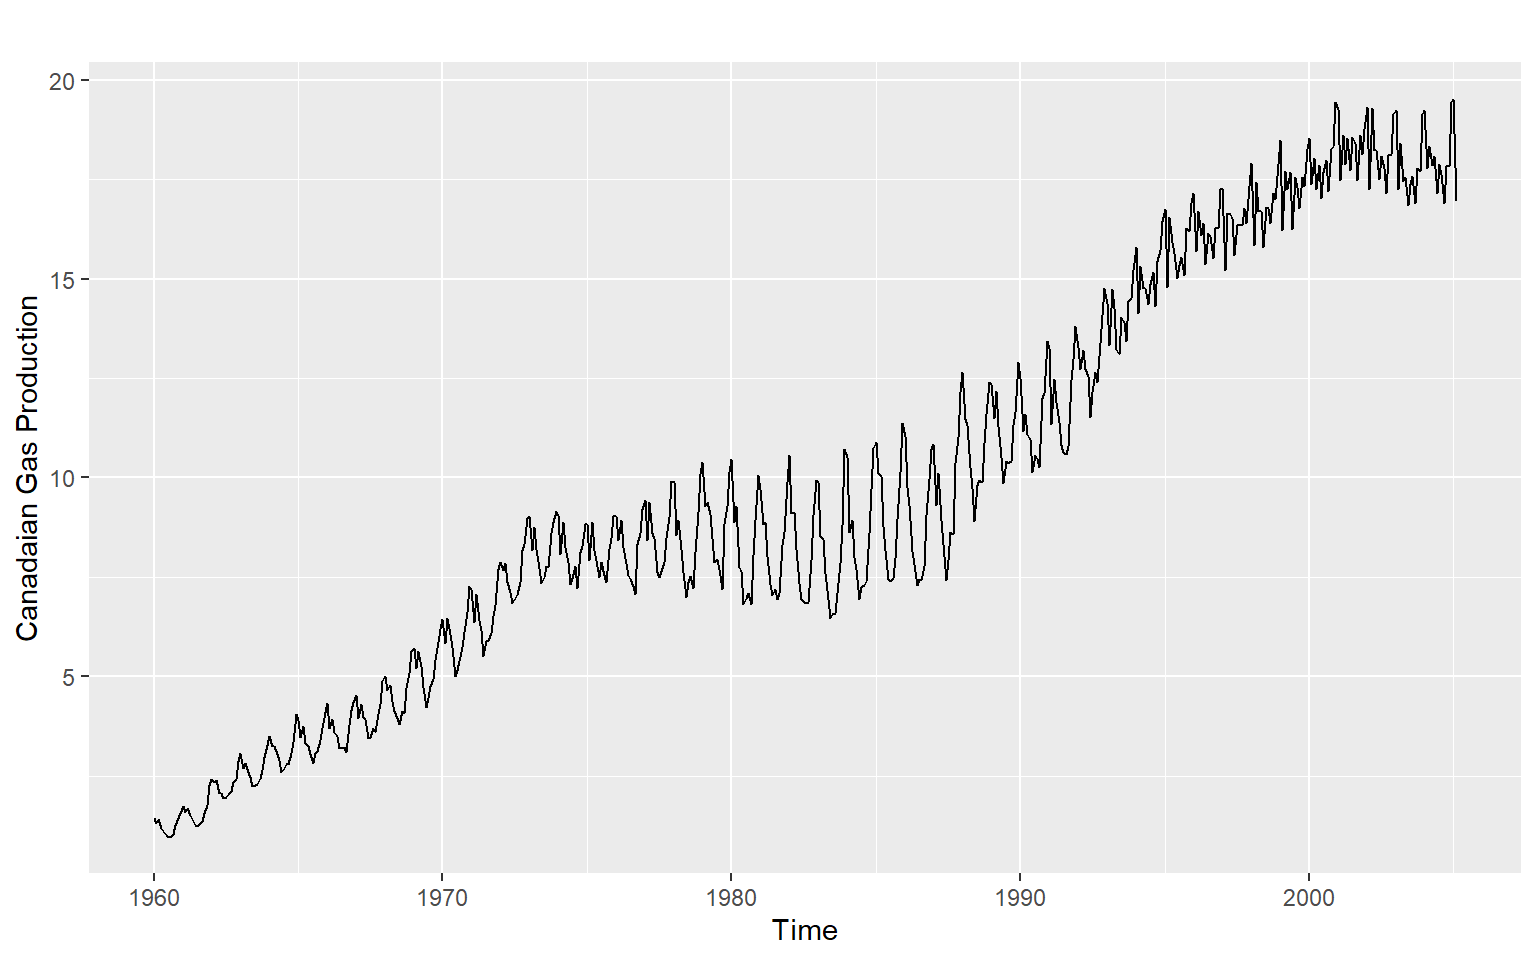
\includegraphics[keepaspectratio]{05-chap5_files/figure-pdf/unnamed-chunk-1-2.pdf}}

\begin{Shaded}
\begin{Highlighting}[]
\NormalTok{p3}
\end{Highlighting}
\end{Shaded}

\pandocbounded{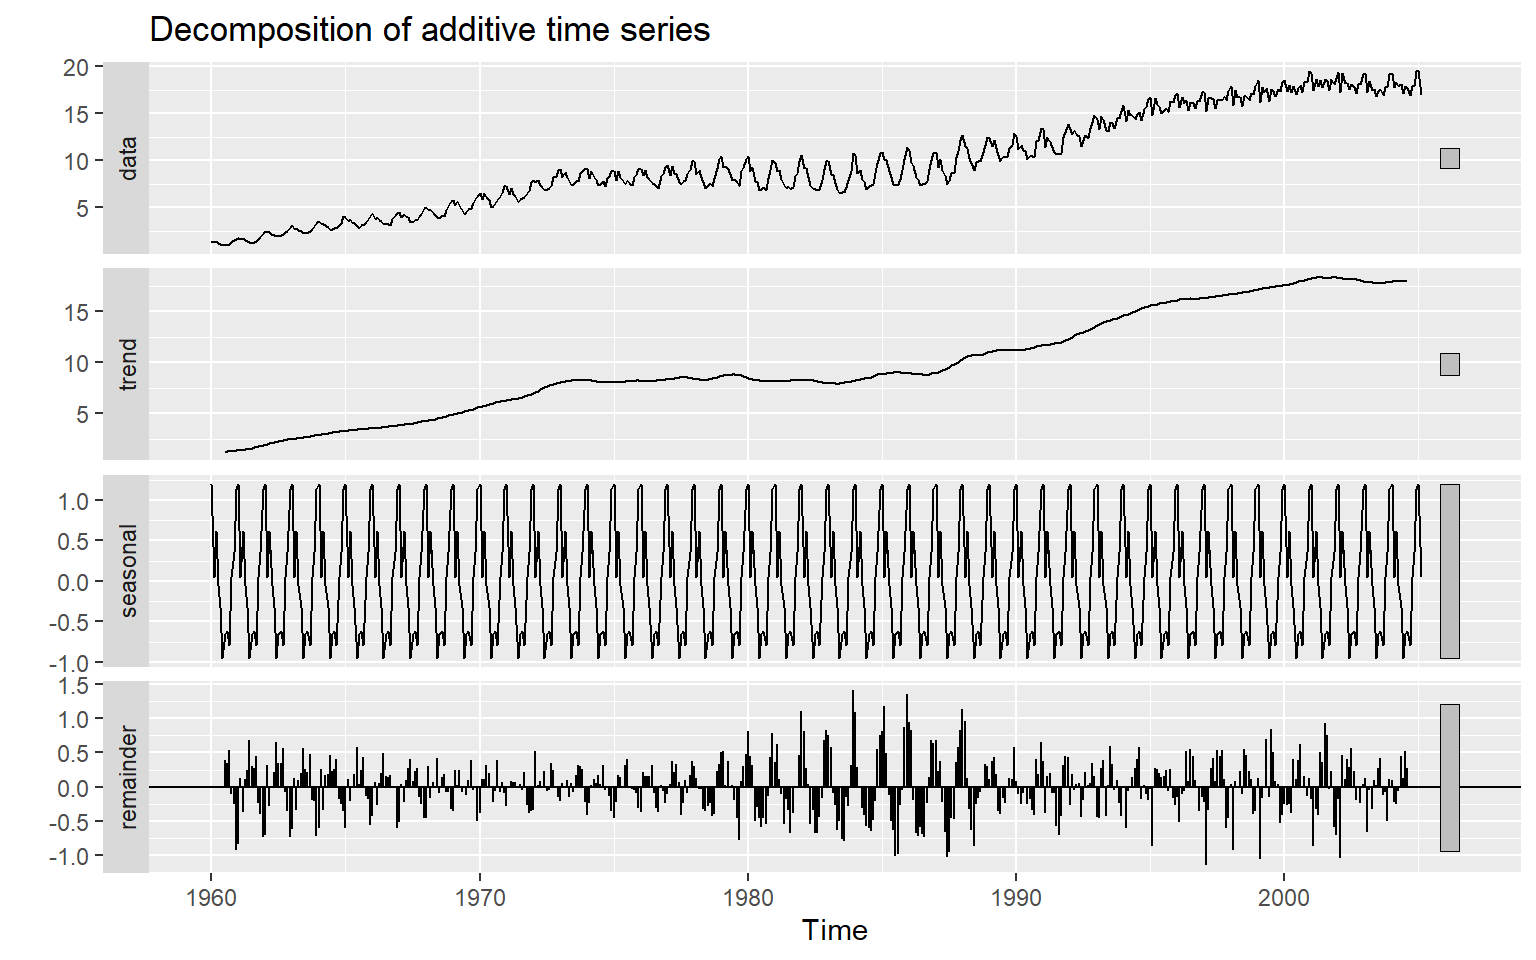
\includegraphics[keepaspectratio]{05-chap5_files/figure-pdf/unnamed-chunk-1-3.pdf}}

\subsection{2. Stochastic trend}\label{stochastic-trend-1}

\begin{itemize}
\item
  A \textbf{stochastic trend} arises from accumulated random shocks.\\
  Example: Random walk

  \[X_t = X_{t-1} + \epsilon_t\]

  where shocks accumulate over time.\\
\item
  Unlike deterministic trends, stochastic trends are unpredictable and
  keep evolving.\\
\item
  Apply non-seasonal differencing to remove stochastic trend.
\item
  Remedy: First differencing usually removes the unit root, yielding
  stationarity.\\
\item
  Testing: Augmented Dickey--Fuller (ADF), Phillips--Perron, or KPSS
  tests.
\end{itemize}

\textbf{Key difference:}\\
- Deterministic trend = predictable pattern (e.g., straight line).\\
- Stochastic trend = unpredictable, driven by random shocks.

\textbf{Non seasonal first-order differencing:} \(Y'_t=Y_t - Y_{t-1}\)

Miss one observation

\textbf{Non seasonal second-order differencing:}
\(Y''_t=Y'_t - Y'_{t-1}\)

Miss two observations

\subsection{3. Seasonality}\label{seasonality}

\begin{itemize}
\item
  Deterministic seasonal pattern → add seasonal dummies or Fourier
  terms.\\
\item
  Stochastic seasonal trend → apply \textbf{seasonal differencing}:
\item
  Seasonal ARIMA (SARIMA) models combine regular and seasonal
  differencing.
\end{itemize}

\textbf{Seasonal differencing:} \(Y_t - Y_{t-m}\)

\begin{itemize}
\item
  To get rid from prominent seasonal components.
\item
  For monthly, \(m=12\), for quarterly, \(m=4\).
\item
  For monthly, we will loose first 12 observations
\item
  Seasonally differenced series will have \(T-m\) observations. Usually
  we do not consider differencing more than twice.
\end{itemize}

\subsection{4. Nonconstant variance}\label{nonconstant-variance}

\begin{itemize}
\tightlist
\item
  Some series show increasing variability over time. The data show
  different variation at different levels of the series.
\item
  Remedies:

  \begin{itemize}
  \tightlist
  \item
    Variance-stabilizing transformations (log, square root, Box--Cox).\\
  \item
    For conditional heteroscedasticity → fit GARCH-type models.
  \end{itemize}
\end{itemize}

\textbf{What differences do you notice?}

\pandocbounded{\includegraphics[keepaspectratio]{05-chap5_files/figure-pdf/unnamed-chunk-3-1.pdf}}

\textbf{Log transformation to stabilize variance}

\begin{Shaded}
\begin{Highlighting}[]
\DocumentationTok{\#\# Original dataset}
\NormalTok{p1 }\OtherTok{\textless{}{-}}\NormalTok{ AirPassengers }\SpecialCharTok{|\textgreater{}}
  \FunctionTok{autoplot}\NormalTok{() }\SpecialCharTok{+}
  \FunctionTok{ggtitle}\NormalTok{(}\StringTok{"Original scale"}\NormalTok{)}

\DocumentationTok{\#\# Transformed dataset}
\NormalTok{AirPassengersBoxCox }\OtherTok{=} \FunctionTok{BoxCox}\NormalTok{(AirPassengers, }\AttributeTok{lambda =} \StringTok{"auto"}\NormalTok{)}

\NormalTok{p2 }\OtherTok{\textless{}{-}}\NormalTok{ AirPassengersBoxCox }\SpecialCharTok{|\textgreater{}}
  \FunctionTok{autoplot}\NormalTok{() }\SpecialCharTok{+}
  \FunctionTok{ggtitle}\NormalTok{(}\FunctionTok{paste0}\NormalTok{(}\StringTok{"Box Cox with lambda = "}\NormalTok{, }
        \FunctionTok{round}\NormalTok{(}\FunctionTok{attributes}\NormalTok{(AirPassengersBoxCox)}\SpecialCharTok{$}\NormalTok{lambda,}\DecValTok{2}\NormalTok{))}
\NormalTok{          )}
\NormalTok{p1}\SpecialCharTok{|}\NormalTok{p2              }
\end{Highlighting}
\end{Shaded}

\pandocbounded{\includegraphics[keepaspectratio]{05-chap5_files/figure-pdf/unnamed-chunk-4-1.pdf}}

\section{Choosing the Order of
Differencing}\label{choosing-the-order-of-differencing}

\begin{itemize}
\tightlist
\item
  Avoid \textbf{over-differencing} (adds unnecessary MA terms and
  inflates variance).\\
\item
  Visual inspection:

  \begin{itemize}
  \tightlist
  \item
    Random walk--like series → first differencing.\\
  \item
    Strong seasonal cycle → seasonal differencing.\\
  \end{itemize}
\item
  Statistical tests (ADF, KPSS) can guide the choice.
\end{itemize}

\section{Models after Differencing}\label{models-after-differencing}

\begin{itemize}
\tightlist
\item
  Once stationarity is achieved, ARMA models can be fitted.\\
\item
  General class:

  \begin{itemize}
  \tightlist
  \item
    \(ARIMA(p,d,q)\)\\
  \item
    Seasonal \(ARIMA (p,d,q)(P,D,Q))_m\)
  \end{itemize}
\item
  Sometimes include drift to capture mean shifts.
\end{itemize}

\section{Seasonal components}\label{seasonal-components}

\begin{itemize}
\tightlist
\item
  The seasonal part of an AR or MA model will be seen in the seasonal
  lags of the PACF and ACF.
\end{itemize}

\textbf{ARIMA(0,0,0)(0,0,1)12 will show}

\begin{itemize}
\item
  a spike at lag 12 in the ACF but no other significant spikes.
\item
  The PACF will show exponential decay in the seasonal lags 12, 24, 36,
  . . . .
\end{itemize}

\textbf{ARIMA(0,0,0)(1,0,0)12 will show}

\begin{itemize}
\item
  exponential decay in the seasonal lags of the ACF.
\item
  a single significant spike at lag 12 in the PACF.
\end{itemize}

\subsection{Practical Examples}\label{practical-examples}

\begin{itemize}
\item
  Simulated series with linear trend → stationary after first
  differencing.
\item
  Monthly series with annual seasonality → stationary after seasonal
  differencing (s=12).
\item
  Log-transformed economic series → removes variance growth, then
  differencing achieves stationarity.
\end{itemize}

\section{Modelling steps}\label{modelling-steps}

\begin{enumerate}
\def\labelenumi{\arabic{enumi}.}
\item
  Plot the data.
\item
  Split time series into training, validation (optional), test.
\item
  If necessary, transform the data (using a Box-Cox transformation) to
  stabilise the variance.
\item
  If the data are non-stationary, take first differences of the data
  until the data are stationary.
\item
  Examine the ACF/PACF to identify a suitable model.
\item
  Try your chosen model(s), and to search for a better model.
\item
  Check the residuals from your chosen model by plotting the ACF of the
  residuals, and doing a portmanteau test of the residuals. If they do
  not look like white noise, try a modified model.
\item
  Once the residuals look like white noise, calculate forecasts.
\end{enumerate}

\section{Example: Model Fitting}\label{example-model-fitting}

\textbf{Step 1: Plot data}

\begin{enumerate}
\def\labelenumi{\arabic{enumi}.}
\item
  Detect unusual observations in the data
\item
  Detect non-stationarity by visual inspections of plots
\end{enumerate}

Stationary series:

\begin{itemize}
\item
  has a constant mean value and fluctuates around the mean.
\item
  constant variance.
\item
  no pattern predictable in the long-term.
\end{itemize}

\textbf{Step 2: Split time series into training and test sets}

\begin{Shaded}
\begin{Highlighting}[]
\NormalTok{training.ap }\OtherTok{\textless{}{-}} \FunctionTok{window}\NormalTok{(AirPassengers, }\AttributeTok{end=}\FunctionTok{c}\NormalTok{(}\DecValTok{1957}\NormalTok{, }\DecValTok{12}\NormalTok{))}
\NormalTok{training.ap}
\end{Highlighting}
\end{Shaded}

\begin{verbatim}
     Jan Feb Mar Apr May Jun Jul Aug Sep Oct Nov Dec
1949 112 118 132 129 121 135 148 148 136 119 104 118
1950 115 126 141 135 125 149 170 170 158 133 114 140
1951 145 150 178 163 172 178 199 199 184 162 146 166
1952 171 180 193 181 183 218 230 242 209 191 172 194
1953 196 196 236 235 229 243 264 272 237 211 180 201
1954 204 188 235 227 234 264 302 293 259 229 203 229
1955 242 233 267 269 270 315 364 347 312 274 237 278
1956 284 277 317 313 318 374 413 405 355 306 271 306
1957 315 301 356 348 355 422 465 467 404 347 305 336
\end{verbatim}

\begin{Shaded}
\begin{Highlighting}[]
\NormalTok{test.ap }\OtherTok{\textless{}{-}} \FunctionTok{window}\NormalTok{(AirPassengers, }\AttributeTok{start=}\FunctionTok{c}\NormalTok{(}\DecValTok{1958}\NormalTok{, }\DecValTok{1}\NormalTok{))}
\NormalTok{test.ap}
\end{Highlighting}
\end{Shaded}

\begin{verbatim}
     Jan Feb Mar Apr May Jun Jul Aug Sep Oct Nov Dec
1958 340 318 362 348 363 435 491 505 404 359 310 337
1959 360 342 406 396 420 472 548 559 463 407 362 405
1960 417 391 419 461 472 535 622 606 508 461 390 432
\end{verbatim}

\begin{Shaded}
\begin{Highlighting}[]
\FunctionTok{autoplot}\NormalTok{(AirPassengers) }\SpecialCharTok{+} 
  \FunctionTok{geom\_vline}\NormalTok{(}\AttributeTok{xintercept =} \DecValTok{1958}\NormalTok{, }\AttributeTok{colour=}\StringTok{"forestgreen"}\NormalTok{)}
\end{Highlighting}
\end{Shaded}

\pandocbounded{\includegraphics[keepaspectratio]{05-chap5_files/figure-pdf/unnamed-chunk-6-1.pdf}}

Training part

\begin{Shaded}
\begin{Highlighting}[]
\FunctionTok{autoplot}\NormalTok{(training.ap)}
\end{Highlighting}
\end{Shaded}

\pandocbounded{\includegraphics[keepaspectratio]{05-chap5_files/figure-pdf/unnamed-chunk-7-1.pdf}}

\textbf{Step 3: Apply transformations}

\begin{Shaded}
\begin{Highlighting}[]
\NormalTok{log.airpassenger }\OtherTok{\textless{}{-}} \FunctionTok{log}\NormalTok{(training.ap)}
\CommentTok{\#log.airpassenger \textless{}{-} BoxCox(training.ap, lambda = 0)}
\FunctionTok{autoplot}\NormalTok{(log.airpassenger)}
\end{Highlighting}
\end{Shaded}

\pandocbounded{\includegraphics[keepaspectratio]{05-chap5_files/figure-pdf/unnamed-chunk-8-1.pdf}}

\textbf{Step 4: Take difference series}

\textbf{Without differencing}

\begin{Shaded}
\begin{Highlighting}[]
\FunctionTok{autoplot}\NormalTok{(log.airpassenger)}
\end{Highlighting}
\end{Shaded}

\pandocbounded{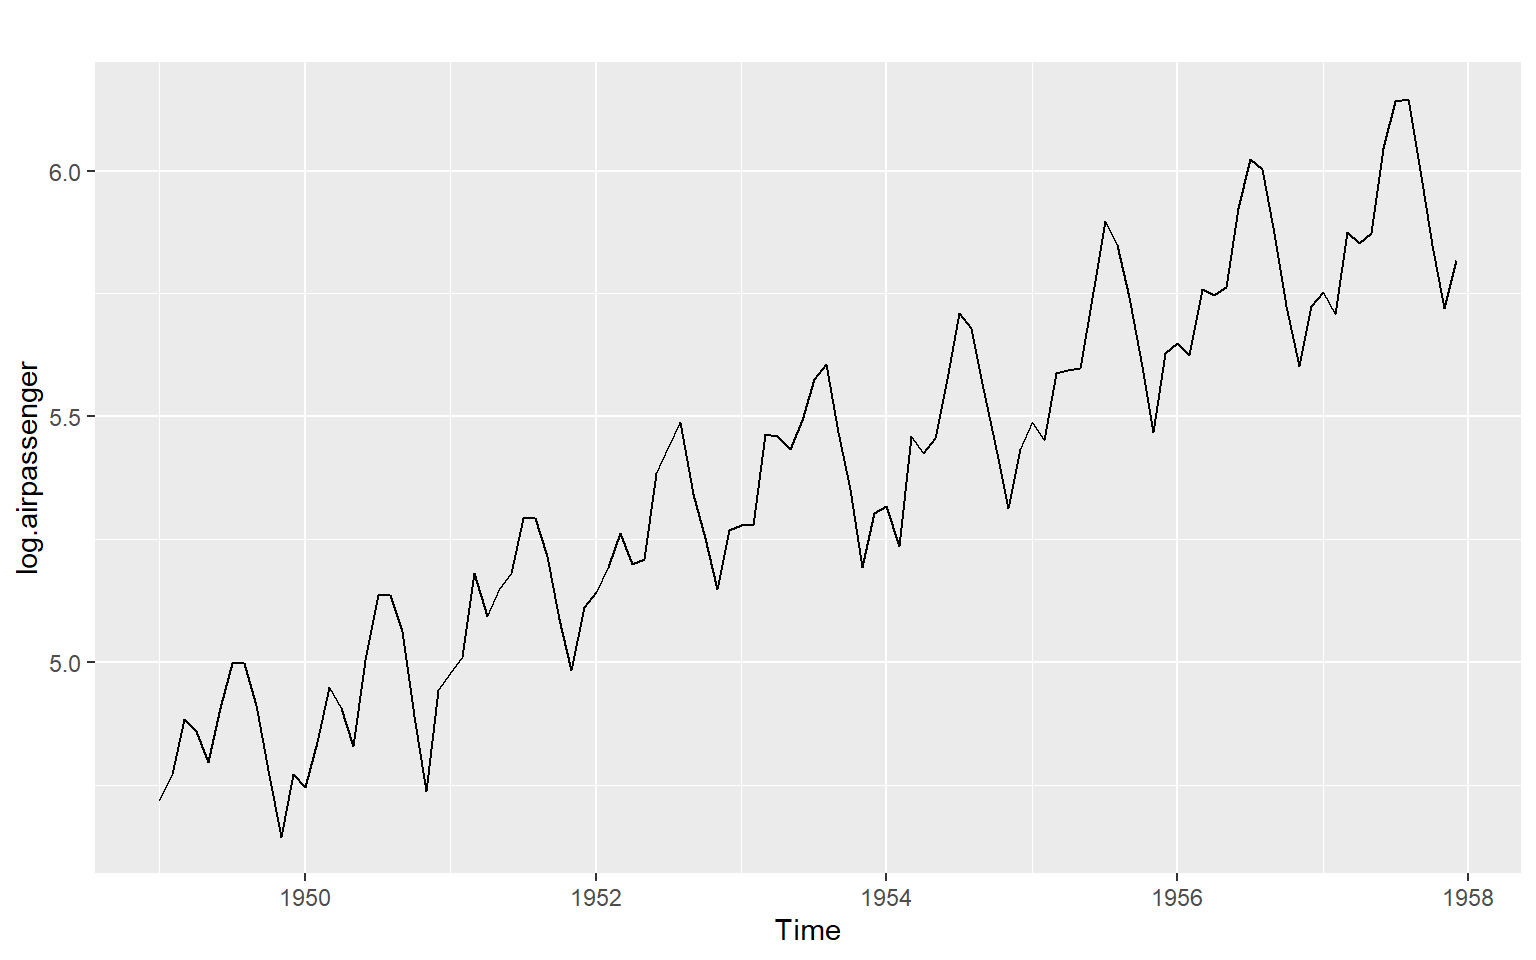
\includegraphics[keepaspectratio]{05-chap5_files/figure-pdf/unnamed-chunk-9-1.pdf}}

\begin{Shaded}
\begin{Highlighting}[]
\FunctionTok{ggAcf}\NormalTok{(log.airpassenger)}
\end{Highlighting}
\end{Shaded}

\pandocbounded{\includegraphics[keepaspectratio]{05-chap5_files/figure-pdf/unnamed-chunk-10-1.pdf}}

\textbf{With differencing}

Seasonal

\begin{Shaded}
\begin{Highlighting}[]
\NormalTok{log.airpassenger }\SpecialCharTok{|\textgreater{}} \FunctionTok{diff}\NormalTok{(}\AttributeTok{lag=}\DecValTok{12}\NormalTok{)  }\SpecialCharTok{|\textgreater{}} \FunctionTok{autoplot}\NormalTok{()}
\end{Highlighting}
\end{Shaded}

\pandocbounded{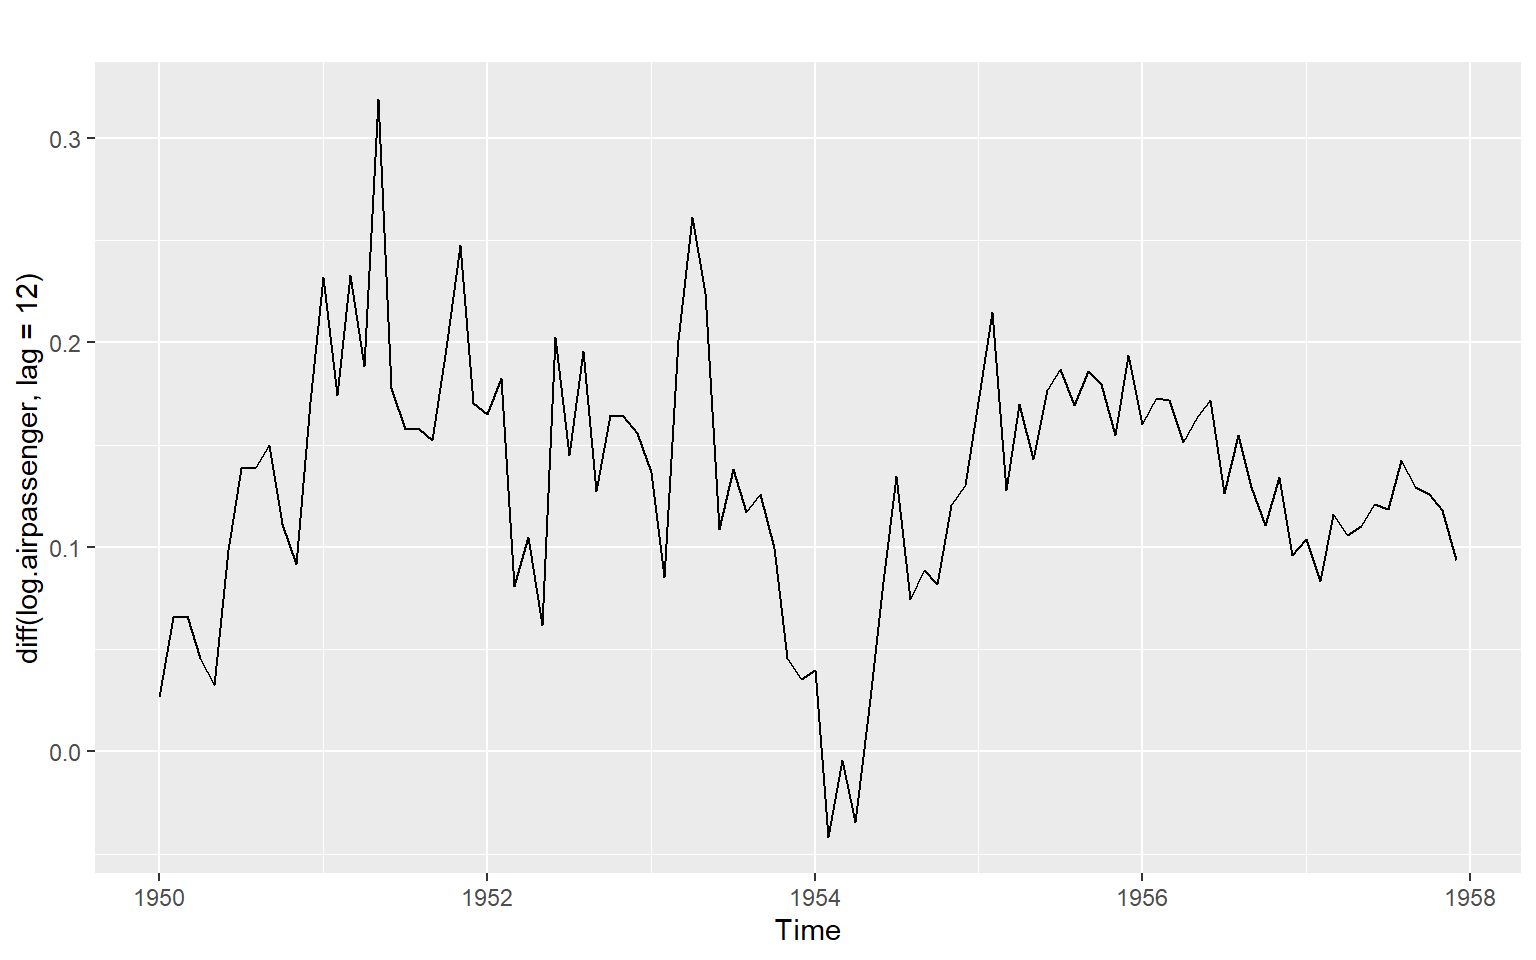
\includegraphics[keepaspectratio]{05-chap5_files/figure-pdf/unnamed-chunk-11-1.pdf}}

\begin{Shaded}
\begin{Highlighting}[]
\NormalTok{log.airpassenger }\SpecialCharTok{|\textgreater{}} \FunctionTok{diff}\NormalTok{(}\AttributeTok{lag=}\DecValTok{12}\NormalTok{)  }\SpecialCharTok{|\textgreater{}} \FunctionTok{ggAcf}\NormalTok{()}
\end{Highlighting}
\end{Shaded}

\pandocbounded{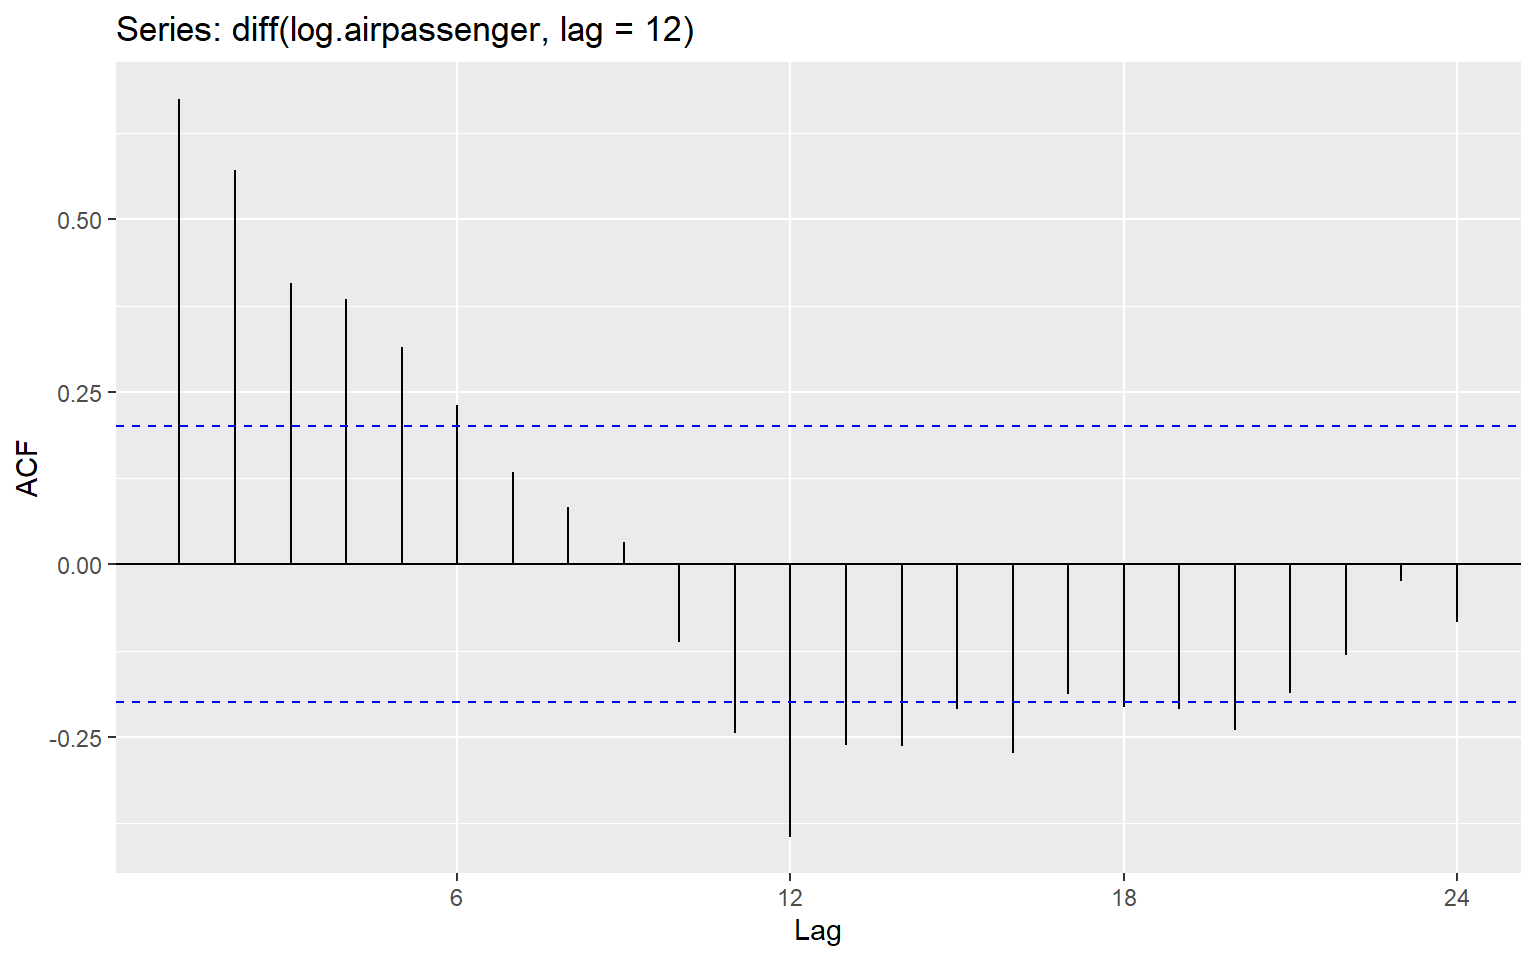
\includegraphics[keepaspectratio]{05-chap5_files/figure-pdf/unnamed-chunk-12-1.pdf}}

Non-seasonal

\begin{Shaded}
\begin{Highlighting}[]
\NormalTok{log.airpassenger }\SpecialCharTok{|\textgreater{}} \FunctionTok{diff}\NormalTok{(}\AttributeTok{lag=}\DecValTok{1}\NormalTok{)  }\SpecialCharTok{|\textgreater{}} \FunctionTok{autoplot}\NormalTok{()}
\end{Highlighting}
\end{Shaded}

\pandocbounded{\includegraphics[keepaspectratio]{05-chap5_files/figure-pdf/unnamed-chunk-13-1.pdf}}

\begin{Shaded}
\begin{Highlighting}[]
\NormalTok{log.airpassenger }\SpecialCharTok{|\textgreater{}} \FunctionTok{diff}\NormalTok{(}\AttributeTok{lag=}\DecValTok{1}\NormalTok{)  }\SpecialCharTok{|\textgreater{}} \FunctionTok{ggAcf}\NormalTok{()}
\end{Highlighting}
\end{Shaded}

\pandocbounded{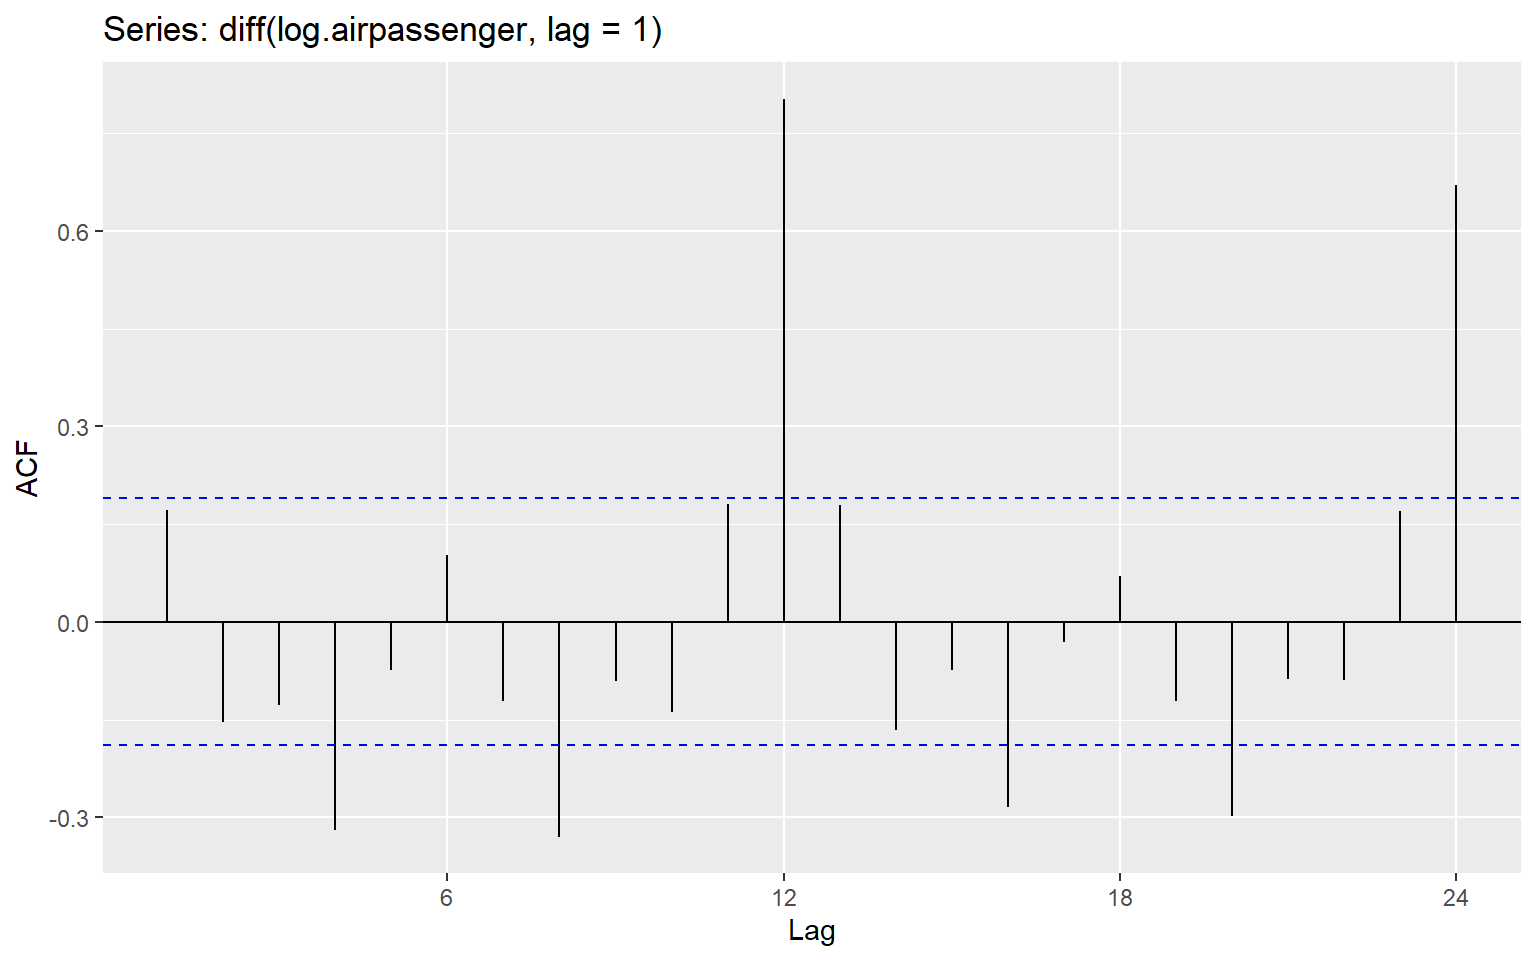
\includegraphics[keepaspectratio]{05-chap5_files/figure-pdf/unnamed-chunk-14-1.pdf}}

Seasonal differencing + Non-seasonal differencing

\begin{Shaded}
\begin{Highlighting}[]
\NormalTok{log.airpassenger }\SpecialCharTok{|\textgreater{}} \FunctionTok{diff}\NormalTok{(}\AttributeTok{lag=}\DecValTok{12}\NormalTok{)  }\SpecialCharTok{|\textgreater{}} \FunctionTok{diff}\NormalTok{(}\AttributeTok{lag=}\DecValTok{1}\NormalTok{) }\SpecialCharTok{|\textgreater{}} \FunctionTok{autoplot}\NormalTok{()}
\end{Highlighting}
\end{Shaded}

\pandocbounded{\includegraphics[keepaspectratio]{05-chap5_files/figure-pdf/unnamed-chunk-15-1.pdf}}

\begin{Shaded}
\begin{Highlighting}[]
\NormalTok{log.airpassenger }\SpecialCharTok{|\textgreater{}} \FunctionTok{diff}\NormalTok{(}\AttributeTok{lag=}\DecValTok{12}\NormalTok{)  }\SpecialCharTok{|\textgreater{}} 
  \FunctionTok{diff}\NormalTok{(}\AttributeTok{lag=}\DecValTok{1}\NormalTok{) }\SpecialCharTok{|\textgreater{}} \FunctionTok{ggAcf}\NormalTok{()}
\end{Highlighting}
\end{Shaded}

\pandocbounded{\includegraphics[keepaspectratio]{05-chap5_files/figure-pdf/unnamed-chunk-16-1.pdf}}

\textbf{Testing for nonstationarity for the presence of unit roots}

\begin{itemize}
\item
  Dickey and Fuller (DF) test
\item
  Augmented DF test
\item
  Phillips and Perron (PP) nonparametric test
\item
  Kwiatkowski-Phillips-Schmidt-Shin (KPSS) test
\end{itemize}

KPSS test

\textbf{H0:} Series is level or trend stationary.

\textbf{H1:} Series is not stationary.

\begin{Shaded}
\begin{Highlighting}[]
\FunctionTok{library}\NormalTok{(urca)}
\NormalTok{diff.sdiff.log.passenger }\OtherTok{\textless{}{-}}\NormalTok{ log.airpassenger }\SpecialCharTok{|\textgreater{}}
  \FunctionTok{diff}\NormalTok{(}\AttributeTok{lag=}\DecValTok{12}\NormalTok{) }\SpecialCharTok{|\textgreater{}}
  \FunctionTok{diff}\NormalTok{(}\AttributeTok{lag=}\DecValTok{1}\NormalTok{)}

\NormalTok{diff.sdiff.log.passenger }\SpecialCharTok{|\textgreater{}}
  \FunctionTok{ur.kpss}\NormalTok{() }\SpecialCharTok{|\textgreater{}}
  \FunctionTok{summary}\NormalTok{()}
\end{Highlighting}
\end{Shaded}

\begin{verbatim}

####################### 
# KPSS Unit Root Test # 
####################### 

Test is of type: mu with 3 lags. 

Value of test-statistic is: 0.0942 

Critical value for a significance level of: 
                10pct  5pct 2.5pct  1pct
critical values 0.347 0.463  0.574 0.739
\end{verbatim}

KPSS test

\begin{Shaded}
\begin{Highlighting}[]
\FunctionTok{ur.kpss}\NormalTok{(log.airpassenger) }\SpecialCharTok{|\textgreater{}} \FunctionTok{summary}\NormalTok{()}
\end{Highlighting}
\end{Shaded}

\begin{verbatim}

####################### 
# KPSS Unit Root Test # 
####################### 

Test is of type: mu with 4 lags. 

Value of test-statistic is: 2.113 

Critical value for a significance level of: 
                10pct  5pct 2.5pct  1pct
critical values 0.347 0.463  0.574 0.739
\end{verbatim}

\begin{Shaded}
\begin{Highlighting}[]
\NormalTok{sdiff.log.airpassenger }\OtherTok{\textless{}{-}}\NormalTok{ training.ap }\SpecialCharTok{|\textgreater{}} \FunctionTok{log}\NormalTok{() }\SpecialCharTok{|\textgreater{}} \FunctionTok{diff}\NormalTok{(}\AttributeTok{lag=}\DecValTok{12}\NormalTok{)}
\FunctionTok{ur.kpss}\NormalTok{(sdiff.log.airpassenger) }\SpecialCharTok{|\textgreater{}} \FunctionTok{summary}\NormalTok{()}
\end{Highlighting}
\end{Shaded}

\begin{verbatim}

####################### 
# KPSS Unit Root Test # 
####################### 

Test is of type: mu with 3 lags. 

Value of test-statistic is: 0.1264 

Critical value for a significance level of: 
                10pct  5pct 2.5pct  1pct
critical values 0.347 0.463  0.574 0.739
\end{verbatim}

\textbf{Step 5: Examine the ACF/PACF to identify a suitable model}

\begin{itemize}
\item
  \(d=1\) and \(D=1\) (from step 3)
\item
  Significant spike at lag 1 in ACF suggests non-seasonal MA(1)
  component.
\item
  Significant spike at lag 12 in ACF suggests seasonal MA(1) component.
\item
  Initial candidate model: \(ARIMA(0,1,1)(0,1,1)_{12}\).
\item
  By analogous logic applied to the PACF, we could also have started
  with \(ARIMA(1,1,0)(1,1,0)_{12}\).
\item
  Let's try both
\end{itemize}

\textbf{Initial model:}

\(ARIMA(0,1,1)(0,1,1)_{12}\)

\(ARIMA(1,1,0)(1,1,0)_{12}\)

\textbf{Try some variations of the initial model:}

\(ARIMA(0,1,1)(1,1,1)_{12}\)

\(ARIMA(1,1,1)(1,1,0)_{12}\)

\(ARIMA(1,1,1)(1,1,1)_{12}\)

Both the ACF and PACF show significant spikes at lag 3, and almost
significant spikes at lag 3, indicating that some additional
non-seasonal terms need to be included in the model.

\(ARIMA(3,1,1)(1,1,1)_{12}\)

\(ARIMA(1,1,3)(1,1,1)_{12}\)

\(ARIMA(3,1,3)(1,1,1)_{12}\)

AICc

\textbf{Initial model: AICc}

\(ARIMA(0,1,1)(0,1,1)_{12}\): -344.33 (the smallest AICc)

\(ARIMA(1,1,0)(1,1,0)_{12}\): -336.32

\textbf{Try some variations of the initial model:}

\(ARIMA(0,1,1)(1,1,1)_{12}\): -342.3 (second smallest AICc)

\(ARIMA(1,1,1)(1,1,0)_{12}\): -336.08

\(ARIMA(1,1,1)(1,1,1)_{12}\): -340.74

\(ARIMA(3,1,1)(1,1,1)_{12}\): -338.89

\(ARIMA(1,1,3)(1,1,1)_{12}\): -339.42

\(ARIMA(3,1,3)(1,1,1)_{12}\): -335.65

\textbf{Step 7: Residual diagnostics}

Fitted values:

\(\hat{Y}_{t|t-1}\): Forecast of \(Y_t\) based on observations
\(Y_1,...Y_t\).

Residuals

\[e_t=Y_t - \hat{Y}_{t|t-1}\]

Assumptions of residuals

\begin{itemize}
\tightlist
\item
  \(\{e_t\}\) uncorrelated. If they aren't, then information left in
  residuals that should be used in computing forecasts.
\end{itemize}

\begin{itemize}
\tightlist
\item
  \(\{e_t\}\) have mean zero. If they don't, then forecasts are biased.
\end{itemize}

\textbf{Useful properties (for prediction intervals)}

\begin{itemize}
\item
  \(\{e_t\}\) have constant variance.
\item
  \(\{e_t\}\) are normally distributed.
\end{itemize}

\textbf{Step 7: Residual diagnostics (cont.)}

H0: Data are not serially correlated.

H1: Data are serially correlated.

\begin{Shaded}
\begin{Highlighting}[]
\NormalTok{fit1 }\OtherTok{\textless{}{-}} \FunctionTok{Arima}\NormalTok{(training.ap, }
              \AttributeTok{order=}\FunctionTok{c}\NormalTok{(}\DecValTok{0}\NormalTok{,}\DecValTok{1}\NormalTok{,}\DecValTok{1}\NormalTok{),}
\AttributeTok{seasonal=}\FunctionTok{c}\NormalTok{(}\DecValTok{0}\NormalTok{,}\DecValTok{1}\NormalTok{,}\DecValTok{1}\NormalTok{), }\AttributeTok{lambda =} \DecValTok{0}\NormalTok{)}
\FunctionTok{checkresiduals}\NormalTok{(fit1)}
\end{Highlighting}
\end{Shaded}

\pandocbounded{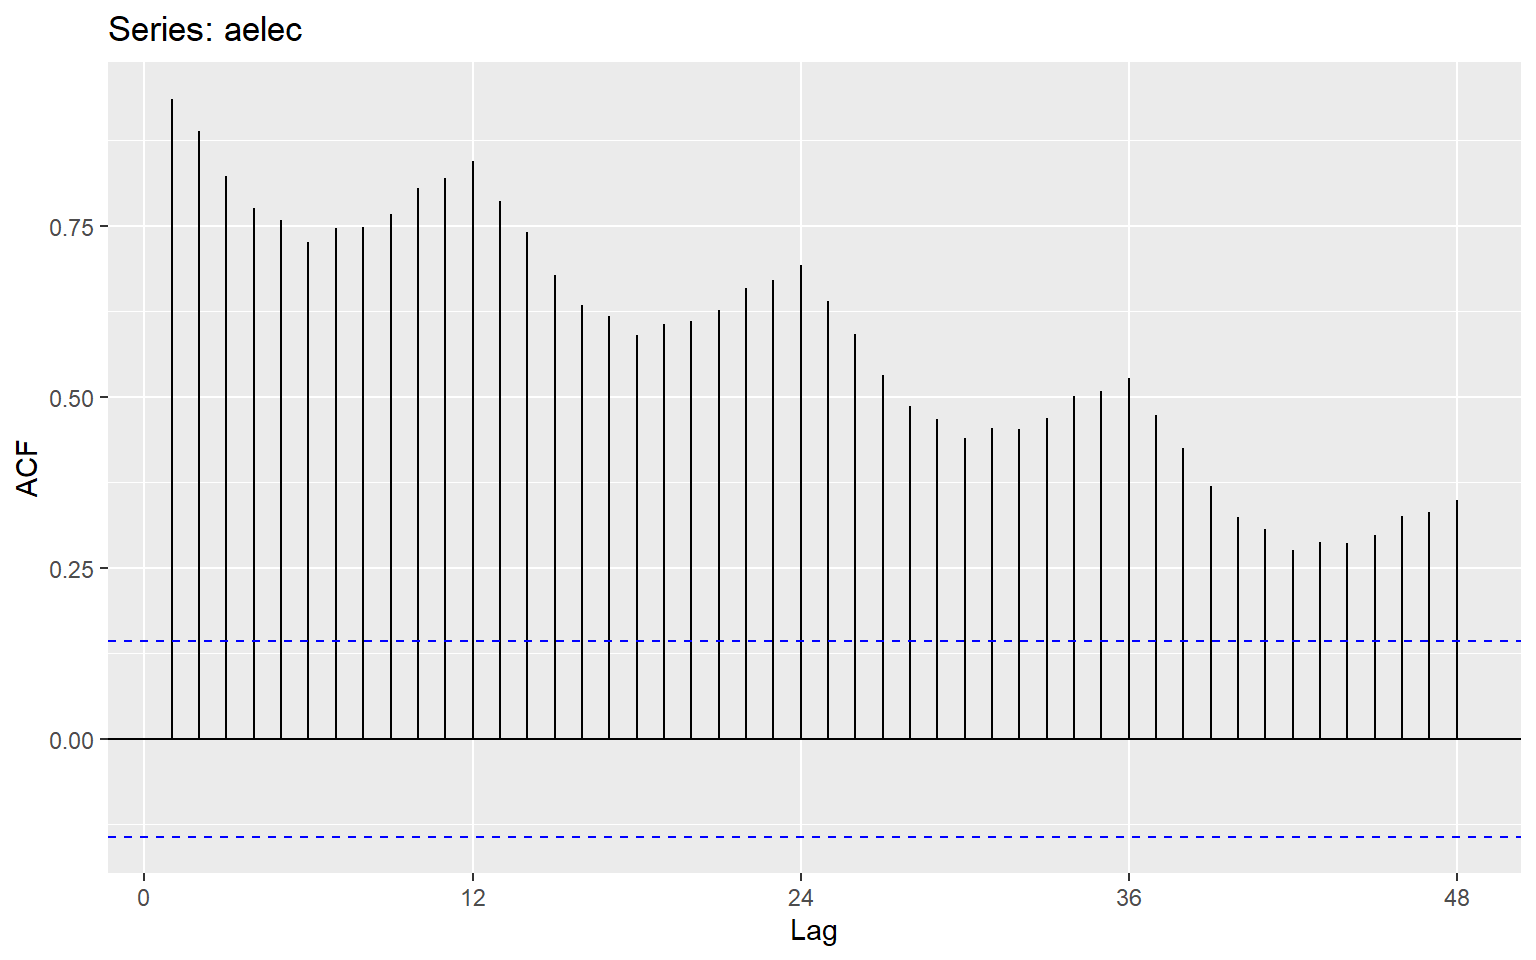
\includegraphics[keepaspectratio]{05-chap5_files/figure-pdf/unnamed-chunk-20-1.pdf}}

\begin{verbatim}

    Ljung-Box test

data:  Residuals from ARIMA(0,1,1)(0,1,1)[12]
Q* = 14.495, df = 20, p-value = 0.8045

Model df: 2.   Total lags used: 22
\end{verbatim}

\begin{Shaded}
\begin{Highlighting}[]
\NormalTok{fit1 }\SpecialCharTok{\%\textgreater{}\%} \FunctionTok{residuals}\NormalTok{() }\SpecialCharTok{\%\textgreater{}\%} \FunctionTok{ggtsdisplay}\NormalTok{()}
\end{Highlighting}
\end{Shaded}

\pandocbounded{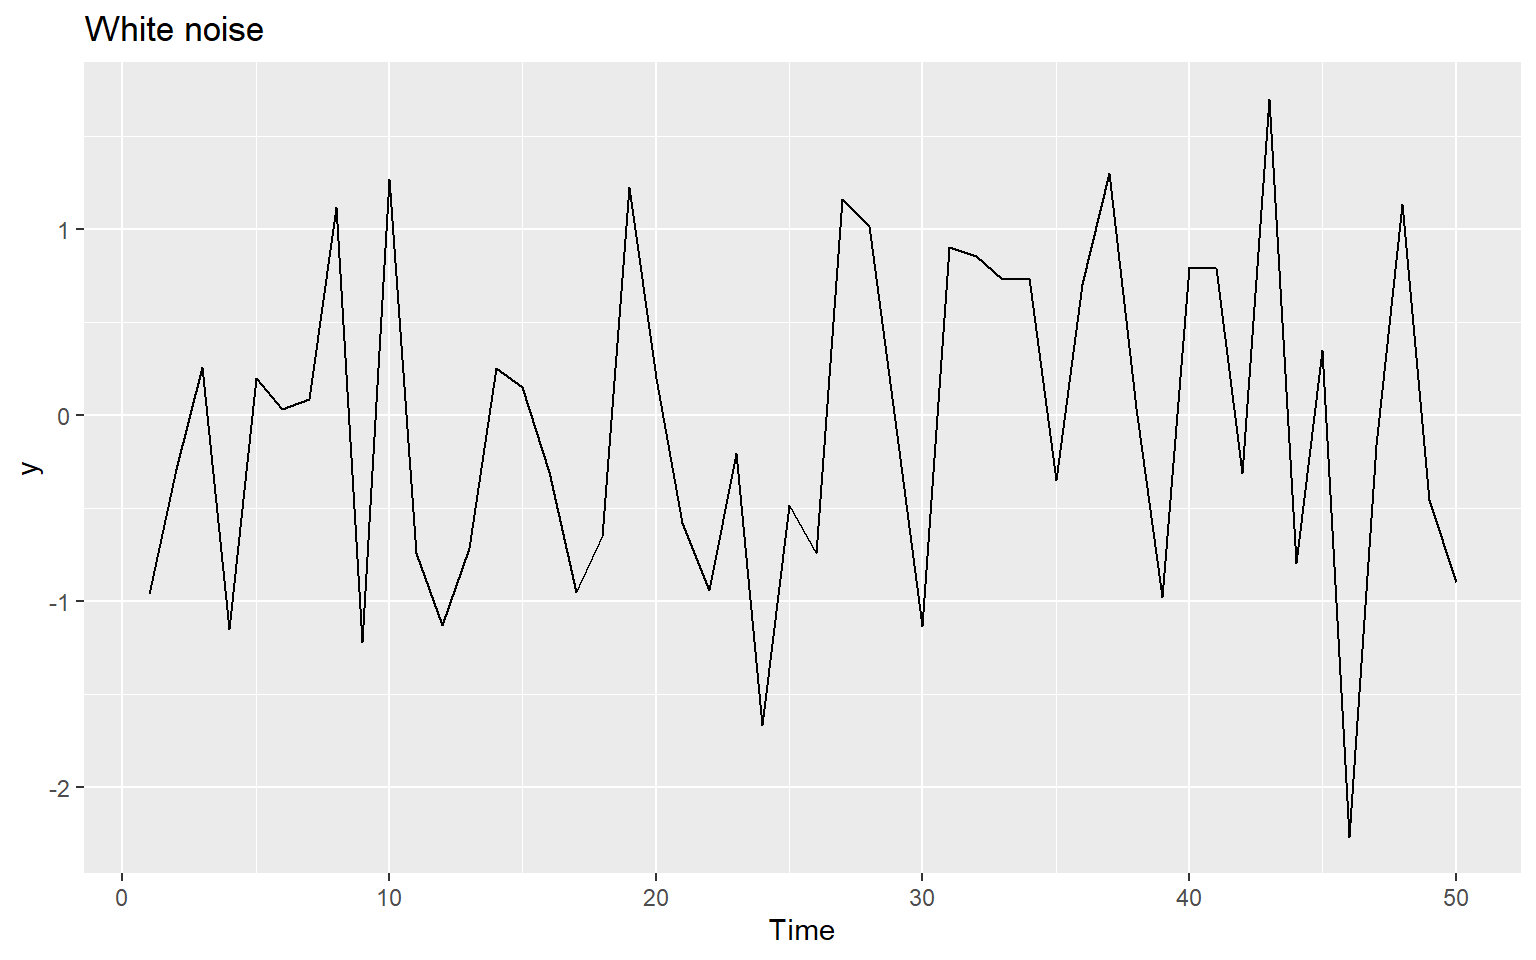
\includegraphics[keepaspectratio]{05-chap5_files/figure-pdf/unnamed-chunk-21-1.pdf}}

\begin{Shaded}
\begin{Highlighting}[]
\NormalTok{fit3 }\OtherTok{\textless{}{-}} \FunctionTok{Arima}\NormalTok{(training.ap, }
              \AttributeTok{order=}\FunctionTok{c}\NormalTok{(}\DecValTok{0}\NormalTok{,}\DecValTok{1}\NormalTok{,}\DecValTok{1}\NormalTok{),}
\AttributeTok{seasonal=}\FunctionTok{c}\NormalTok{(}\DecValTok{1}\NormalTok{,}\DecValTok{1}\NormalTok{,}\DecValTok{1}\NormalTok{), }\AttributeTok{lambda =} \DecValTok{0}\NormalTok{)}
\FunctionTok{checkresiduals}\NormalTok{(fit3)}
\end{Highlighting}
\end{Shaded}

\pandocbounded{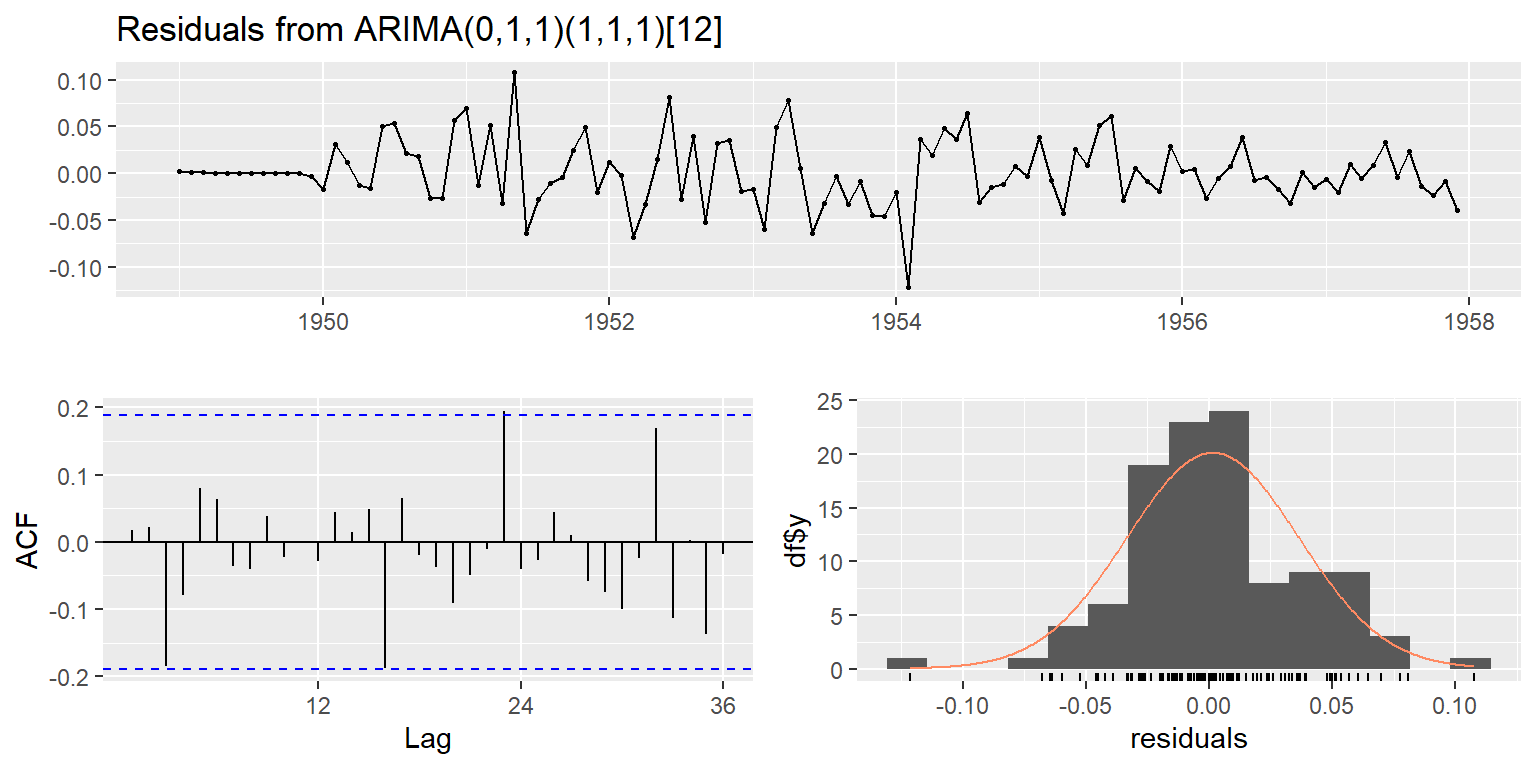
\includegraphics[keepaspectratio]{05-chap5_files/figure-pdf/unnamed-chunk-22-1.pdf}}

\begin{verbatim}

    Ljung-Box test

data:  Residuals from ARIMA(0,1,1)(1,1,1)[12]
Q* = 13.971, df = 19, p-value = 0.7854

Model df: 3.   Total lags used: 22
\end{verbatim}

\begin{Shaded}
\begin{Highlighting}[]
\NormalTok{fit3 }\SpecialCharTok{\%\textgreater{}\%} \FunctionTok{residuals}\NormalTok{() }\SpecialCharTok{\%\textgreater{}\%} \FunctionTok{ggtsdisplay}\NormalTok{()}
\end{Highlighting}
\end{Shaded}

\pandocbounded{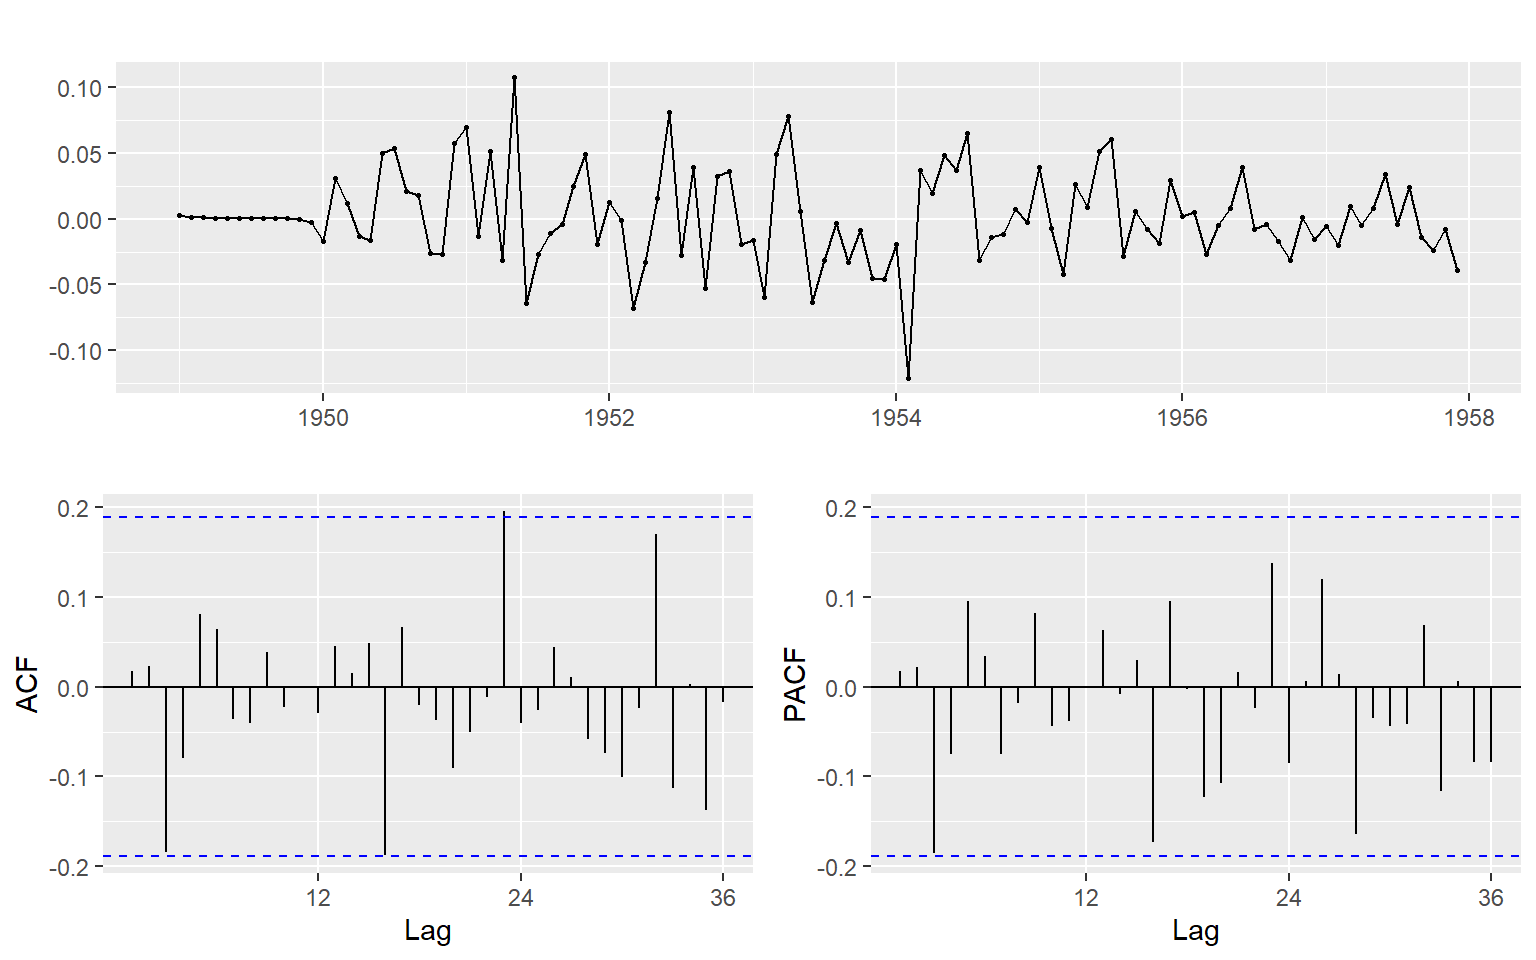
\includegraphics[keepaspectratio]{05-chap5_files/figure-pdf/unnamed-chunk-23-1.pdf}}

\textbf{Step 8: Calculate forecasts}

\(ARIMA(0,1,1)(0,1,1)_{12}\)

\begin{Shaded}
\begin{Highlighting}[]
\NormalTok{fit1 }\SpecialCharTok{\%\textgreater{}\%} \FunctionTok{forecast}\NormalTok{(}\AttributeTok{h=}\DecValTok{36}\NormalTok{) }\SpecialCharTok{\%\textgreater{}\%} 
  \FunctionTok{autoplot}\NormalTok{()}
\end{Highlighting}
\end{Shaded}

\pandocbounded{\includegraphics[keepaspectratio]{05-chap5_files/figure-pdf/unnamed-chunk-24-1.pdf}}

\(ARIMA(0,1,1)(1,1,1)_{12}\)

\begin{Shaded}
\begin{Highlighting}[]
\NormalTok{fit3 }\SpecialCharTok{\%\textgreater{}\%} \FunctionTok{forecast}\NormalTok{(}\AttributeTok{h=}\DecValTok{36}\NormalTok{) }\SpecialCharTok{\%\textgreater{}\%} 
  \FunctionTok{autoplot}\NormalTok{()}
\end{Highlighting}
\end{Shaded}

\pandocbounded{\includegraphics[keepaspectratio]{05-chap5_files/figure-pdf/unnamed-chunk-25-1.pdf}}

\(ARIMA(0,1,1)(0,1,1)_{12}\)

\begin{Shaded}
\begin{Highlighting}[]
\NormalTok{fit1.forecast }\OtherTok{\textless{}{-}}\NormalTok{ fit1 }\SpecialCharTok{\%\textgreater{}\%} \FunctionTok{forecast}\NormalTok{(}\AttributeTok{h=}\DecValTok{36}\NormalTok{) }
\NormalTok{fit1.forecast}\SpecialCharTok{$}\NormalTok{mean}
\end{Highlighting}
\end{Shaded}

\begin{verbatim}
          Jan      Feb      Mar      Apr      May      Jun      Jul      Aug
1958 350.6592 339.1766 396.7654 389.3934 394.7295 460.6986 512.2818 507.5185
1959 394.8025 381.8745 446.7129 438.4129 444.4207 518.6945 576.7713 571.4083
1960 444.5029 429.9474 502.9482 493.6032 500.3674 583.9912 649.3792 643.3411
          Sep      Oct      Nov      Dec
1958 445.0042 386.2473 339.3564 381.5803
1959 501.0243 434.8708 382.0769 429.6162
1960 564.0966 489.6152 430.1753 483.6992
\end{verbatim}

\(ARIMA(0,1,1)(1,1,1)_{12}\)

\begin{Shaded}
\begin{Highlighting}[]
\NormalTok{fit3.forecast }\OtherTok{\textless{}{-}}\NormalTok{ fit3 }\SpecialCharTok{\%\textgreater{}\%} \FunctionTok{forecast}\NormalTok{(}\AttributeTok{h=}\DecValTok{36}\NormalTok{) }
\NormalTok{fit3.forecast}\SpecialCharTok{$}\NormalTok{mean}
\end{Highlighting}
\end{Shaded}

\begin{verbatim}
          Jan      Feb      Mar      Apr      May      Jun      Jul      Aug
1958 351.0115 339.0589 396.3161 389.4484 395.0305 461.6590 513.6099 507.9900
1959 395.2760 381.5215 446.3245 438.4261 444.8906 520.5608 578.7432 573.0358
1960 444.7886 429.3347 502.2289 493.3544 500.6143 585.7116 651.2077 644.7354
          Sep      Oct      Nov      Dec
1958 445.3297 386.3269 339.4872 381.8812
1959 501.8766 435.0725 382.3290 429.4328
1960 564.7108 489.5677 430.2174 483.2724
\end{verbatim}

\textbf{Step 9: Evaluate forecast accuracy}

How well our model is doing for out-of-sample?

Forecast error = True value - Observed value

\[e_{T+h}=Y_{T+h}-\hat{Y}_{T+h|T}\]

Where,

\(Y_{T+h}\): \((T+h)^{th}\) observation, \(h=1,..., H\)

\(\hat{Y}_{T+h|T}\): Forecast based on data uo to time \(T\).

\begin{itemize}
\item
  \textbf{True} forecast error as the test data is not used in computing
  \(\hat{Y}_{T+h|T}\).
\item
  Unlike, residuals, forecast errors on the test set involve multi-step
  forecasts.
\item
  Use forecast error measures to evaluate the models.
\end{itemize}

\(ARIMA(0,1,1)(0,1,1)_{12}\)

\begin{Shaded}
\begin{Highlighting}[]
\NormalTok{fit1.forecast }\OtherTok{\textless{}{-}}\NormalTok{ fit1 }\SpecialCharTok{|\textgreater{}} 
  \FunctionTok{forecast}\NormalTok{(}\AttributeTok{h=}\DecValTok{36}\NormalTok{) }
\end{Highlighting}
\end{Shaded}

\begin{Shaded}
\begin{Highlighting}[]
\FunctionTok{accuracy}\NormalTok{(fit1.forecast}\SpecialCharTok{$}\NormalTok{mean, test.ap)}
\end{Highlighting}
\end{Shaded}

\begin{verbatim}
                ME   RMSE      MAE       MPE     MAPE       ACF1 Theil's U
Test set -33.71566 36.559 33.71566 -8.112567 8.112567 0.08524612 0.7974916
\end{verbatim}

\(ARIMA(0,1,1)(1,1,1)_{12}\)

\begin{Shaded}
\begin{Highlighting}[]
\NormalTok{fit3.forecast }\OtherTok{\textless{}{-}}\NormalTok{ fit3 }\SpecialCharTok{|\textgreater{}}
  \FunctionTok{forecast}\NormalTok{(}\AttributeTok{h=}\DecValTok{36}\NormalTok{) }
\end{Highlighting}
\end{Shaded}

\begin{Shaded}
\begin{Highlighting}[]
\FunctionTok{accuracy}\NormalTok{(fit3.forecast}\SpecialCharTok{$}\NormalTok{mean, test.ap)}
\end{Highlighting}
\end{Shaded}

\begin{verbatim}
                ME     RMSE      MAE       MPE     MAPE       ACF1 Theil's U
Test set -34.12174 36.87661 34.12174 -8.190874 8.190874 0.06782644 0.8019226
\end{verbatim}

\(ARIMA(0,1,1)(0,1,1)_{12}\) MAE, MAPE is smaller than
\(ARIMA(0,1,1)(1,1,1)_{12}\). Hence, we select
\(ARIMA(0,1,1)(0,1,1)_{12}\) to forecast future values.

\section{\texorpdfstring{\texttt{auto.arima}}{auto.arima}}\label{auto.arima}

Your turn: Explain the steps and logic behind the auto.arima() function
in R for automatically identifying the appropriate ARIMA/SARIMA model.

\section{Reading}\label{reading}

\url{https://jtr13.github.io/cc19/visualization-in-time-series-analysis.html}

\bookmarksetup{startatroot}

\chapter{Time Series Decomposition}\label{sec-intro}

Decompose a time series into seasonal, trend and irregular components

\section{Different Methods in Time Series
Decomposition}\label{different-methods-in-time-series-decomposition}

\begin{enumerate}
\def\labelenumi{\arabic{enumi}.}
\tightlist
\item
  \texttt{stats::decompose(ts\_data,\ type\ =\ c(“additive”,\ “multiplicative”))}
  Decompose a time series into seasonal, trend and irregular components
  using moving average.
\end{enumerate}

\begin{Shaded}
\begin{Highlighting}[]
\FunctionTok{library}\NormalTok{(forecast)}
\FunctionTok{library}\NormalTok{(expsmooth) }\CommentTok{\# use a dataset cangas here}
\FunctionTok{library}\NormalTok{(ggplot2)}
\NormalTok{ts\_data }\OtherTok{=}\NormalTok{ cangas}
\NormalTok{ts\_data }\SpecialCharTok{|\textgreater{}} \FunctionTok{ggAcf}\NormalTok{()}
\end{Highlighting}
\end{Shaded}

\pandocbounded{\includegraphics[keepaspectratio]{06-chap6_files/figure-pdf/unnamed-chunk-1-1.pdf}}

\begin{Shaded}
\begin{Highlighting}[]
\FunctionTok{autoplot}\NormalTok{(ts\_data) }\SpecialCharTok{+} \FunctionTok{ylab}\NormalTok{(}\StringTok{"Canadaian Gas Production"}\NormalTok{)}
\end{Highlighting}
\end{Shaded}

\pandocbounded{\includegraphics[keepaspectratio]{06-chap6_files/figure-pdf/unnamed-chunk-1-2.pdf}}

\begin{Shaded}
\begin{Highlighting}[]
\NormalTok{fit }\OtherTok{\textless{}{-}} \FunctionTok{decompose}\NormalTok{(ts\_data, }\AttributeTok{type=}\StringTok{\textquotesingle{}additive\textquotesingle{}}\NormalTok{)}
\FunctionTok{autoplot}\NormalTok{(fit)}
\end{Highlighting}
\end{Shaded}

\pandocbounded{\includegraphics[keepaspectratio]{06-chap6_files/figure-pdf/unnamed-chunk-1-3.pdf}}

\begin{enumerate}
\def\labelenumi{\arabic{enumi}.}
\setcounter{enumi}{1}
\tightlist
\item
  \texttt{stats::stl(ts\_data,\ s.window)} Decompose a time series into
  seasonal, trend and irregular components using loess.
\end{enumerate}

\begin{verbatim}
$time.series
            seasonal      trend     remainder
Jan 1960  1.02190188  0.7495630 -0.3408648970
Feb 1960  0.20665601  0.8812904  0.2179535567
Mar 1960  0.61819325  1.0130179 -0.2290110999
Apr 1960 -0.02921181  1.1287898  0.0703220314
May 1960 -0.28773303  1.2445617  0.1592713174
Jun 1960 -0.89898935  1.3429699  0.5673194168
Jul 1960 -0.63692484  1.4413782  0.1615466876
Aug 1960 -0.57260730  1.4087335  0.1411738201
Sep 1960 -0.76779277  1.3760888  0.4228039756
Oct 1960  0.06059580  1.3051534 -0.1136492129
Nov 1960  0.32721448  1.2342180 -0.1195325095
Dec 1960  0.95869770  1.2179881 -0.6129857933
Jan 1961  1.02190188  1.2017582 -0.4786600422
Feb 1961  0.20665601  1.2755296  0.1013143468
Mar 1961  0.61819325  1.3493011 -0.2904943745
Apr 1961 -0.02921181  1.4833129  0.0613988666
May 1961 -0.28773303  1.6173248  0.0755082623
Jun 1961 -0.89898935  1.6856974  0.4596919686
Jul 1961 -0.63692484  1.7540700  0.1066548463
Aug 1961 -0.57260730  1.7361382  0.1281691055
Sep 1961 -0.76779277  1.7182064  0.4036863876
Oct 1961  0.06059580  1.6938172 -0.1992130190
Nov 1961  0.32721448  1.6694281 -0.2318425338
Dec 1961  0.95869770  1.6979770 -0.4017747077
Jan 1962  1.02190188  1.7265260 -0.3320278467
Feb 1962  0.20665601  1.8507321  0.2910118732
Mar 1962  0.61819325  1.9749383 -0.2079315172
Apr 1962 -0.02921181  2.1348259 -0.0405140958
May 1962 -0.28773303  2.2947136  0.0524194802
Jun 1962 -0.89898935  2.3716658  0.4536235699
Jul 1962 -0.63692484  2.4486180  0.1514068310
Aug 1962 -0.57260730  2.4336911  0.1785161790
Sep 1962 -0.76779277  2.4187642  0.4594285500
Oct 1962  0.06059580  2.3659325 -0.0838282531
Nov 1962  0.32721448  2.3131007 -0.2183151643
Dec 1962  0.95869770  2.2998369 -0.4031345652
Jan 1963  1.02190188  2.2865731 -0.2518749312
Feb 1963  0.20665601  2.3670754  0.1060686060
Mar 1963  0.61819325  2.4475777 -0.2556709669
Apr 1963 -0.02921181  2.5676341  0.0478777517
May 1963 -0.28773303  2.6876904  0.0674426249
Jun 1963 -0.89898935  2.7501480  0.3895413148
Jul 1963 -0.63692484  2.8126057  0.0905191759
Aug 1963 -0.57260730  2.7971426  0.0643646638
Sep 1963 -0.76779277  2.7816796  0.4166131747
Oct 1963  0.06059580  2.7486907 -0.1747865003
Nov 1963  0.32721448  2.7157018 -0.0713162834
Dec 1963  0.95869770  2.7278607 -0.4288584304
Jan 1964  1.02190188  2.7400197 -0.2747215425
Feb 1964  0.20665601  2.8251743  0.2003697342
Mar 1964  0.61819325  2.9103289 -0.2821220992
Apr 1964 -0.02921181  3.0270372  0.1125746291
May 1964 -0.28773303  3.1437455  0.0277875121
Jun 1964 -0.89898935  3.2008458  0.2901435384
Jul 1964 -0.63692484  3.2579461  0.0785787362
Aug 1964 -0.57260730  3.2476167  0.1209905662
Sep 1964 -0.76779277  3.2372874  0.3265054191
Oct 1964  0.06059580  3.2023293 -0.1893251192
Nov 1964  0.32721448  3.1673713 -0.1546857657
Dec 1964  0.95869770  3.1626102 -0.0648079081
Jan 1965  1.02190188  3.1578491 -0.2790510155
Feb 1965  0.20665601  3.2217406  0.0503033640
Mar 1965  0.61819325  3.2856321 -0.1475253667
Apr 1965 -0.02921181  3.3695284 -0.0231166124
May 1965 -0.28773303  3.4534247  0.0892082966
Jun 1965 -0.89898935  3.4994649  0.4306244062
Jul 1965 -0.63692484  3.5455052 -0.0899803129
Aug 1965 -0.57260730  3.5288551  0.1229521531
Sep 1965 -0.76779277  3.5122051  0.3772876421
Oct 1965  0.06059580  3.4724795 -0.1393752913
Nov 1965  0.32721448  3.4327539 -0.0688683328
Dec 1965  0.95869770  3.4238297 -0.2835273632
Jan 1966  1.02190188  3.4149055 -0.1026073586
Feb 1966  0.20665601  3.4741911  0.0102528504
Mar 1966  0.61819325  3.5334768 -0.2169700507
Apr 1966 -0.02921181  3.6102576  0.0165542042
May 1966 -0.28773303  3.6870384  0.0991946139
Jun 1966 -0.89898935  3.7363302  0.3636591285
Jul 1966 -0.63692484  3.7856220  0.0325028144
Aug 1966 -0.57260730  3.7784050  0.0037022479
Sep 1966 -0.76779277  3.7711881  0.0985047044
Oct 1966  0.06059580  3.7375745 -0.0277702735
Nov 1966  0.32721448  3.7039609  0.1188246404
Dec 1966  0.95869770  3.7170618 -0.3274595432
Jan 1967  1.02190188  3.7301628 -0.2309646919
Feb 1967  0.20665601  3.7923380 -0.0443940394
Mar 1967  0.61819325  3.8545132 -0.1640064971
Apr 1967 -0.02921181  3.9459145  0.0661973247
May 1967 -0.28773303  4.0373157  0.1625173012
Jun 1967 -0.89898935  4.0926080  0.2481813303
Jul 1967 -0.63692484  4.1479003 -0.0521754692
Aug 1967 -0.57260730  4.1403764  0.1177308519
Sep 1967 -0.76779277  4.1328526  0.2410401958
Oct 1967  0.06059580  4.1229499 -0.1326457065
Nov 1967  0.32721448  4.1130472 -0.1514617170
Dec 1967  0.95869770  4.1319290 -0.2012267057
Jan 1968  1.02190188  4.1508108 -0.1785126595
Feb 1968  0.20665601  4.2199187  0.2135253022
Mar 1968  0.61819325  4.2890266 -0.1311198462
Apr 1968 -0.02921181  4.3758947  0.0328171206
May 1968 -0.28773303  4.4627628 -0.0590297580
Jun 1968 -0.89898935  4.5287932  0.3247961276
Jul 1968 -0.63692484  4.5948237 -0.1505988154
Aug 1968 -0.57260730  4.6372644  0.0570429218
Sep 1968 -0.76779277  4.6797051  0.1502876819
Oct 1968  0.06059580  4.7174649 -0.0727607294
Nov 1968  0.32721448  4.7552248  0.0023607512
Dec 1968  0.95869770  4.8110562 -0.1240538538
Jan 1969  1.02190188  4.8668875 -0.1693894239
Feb 1969  0.20665601  4.9230950  0.0882490180
Mar 1969  0.61819325  4.9793024  0.0369043497
Apr 1969 -0.02921181  5.0508679  0.2303439518
May 1969 -0.28773303  5.1224333 -0.1096002915
Jun 1969 -0.89898935  5.1876961 -0.0622067978
Jul 1969 -0.63692484  5.2529590 -0.1629341327
Aug 1969 -0.57260730  5.2960406  0.0384666733
Sep 1969 -0.76779277  5.3391223  0.3690705023
Oct 1969  0.06059580  5.3976369 -0.0447326595
Nov 1969  0.32721448  5.4561514  0.0748340706
Dec 1969  0.95869770  5.5290826 -0.2896803162
Jan 1970  1.02190188  5.6020138 -0.1765156680
Feb 1970  0.20665601  5.6737729 -0.0392288827
Mar 1970  0.61819325  5.7455320  0.1063747923
Apr 1970 -0.02921181  5.8227338  0.2714780311
May 1970 -0.28773303  5.8999356  0.1326974246
Jun 1970 -0.89898935  5.9631716 -0.0699822074
Jul 1970 -0.63692484  6.0264075 -0.2451826680
Aug 1970 -0.57260730  6.0661360 -0.1055287121
Sep 1970 -0.76779277  6.1058645  0.3841282666
Oct 1970  0.06059580  6.1523189 -0.0913147306
Nov 1970  0.32721448  6.1987734  0.0970121640
Dec 1970  0.95869770  6.2420990  0.0710032964
Jan 1971  1.02190188  6.2854247 -0.1120265364
Feb 1971  0.20665601  6.3170879 -0.1613439504
Mar 1971  0.61819325  6.3487512  0.1065555254
Apr 1971 -0.02921181  6.3910290  0.0544828552
May 1971 -0.28773303  6.4333067  0.0214263396
Jun 1971 -0.89898935  6.4727120 -0.0668226568
Jul 1971 -0.63692484  6.5121173  0.0085075183
Aug 1971 -0.57260730  6.5466074 -0.0591001277
Sep 1971 -0.76779277  6.5810975  0.2828952492
Oct 1971  0.06059580  6.6649446 -0.2016403959
Nov 1971  0.32721448  6.7487917 -0.2802061492
Dec 1971  0.95869770  6.8561211 -0.1153187557
Jan 1972  1.02190188  6.9634505 -0.1102523273
Feb 1972  0.20665601  7.0980726  0.3720713766
Mar 1972  0.61819325  7.2326948  0.0072119703
Apr 1972 -0.02921181  7.3601441  0.0286677162
May 1972 -0.28773303  7.4875934 -0.0725603832
Jun 1972 -0.89898935  7.5937731  0.1549162582
Jul 1972 -0.63692484  7.6999528 -0.1000279290
Aug 1972 -0.57260730  7.7825557 -0.1364484465
Sep 1972 -0.76779277  7.8651587  0.2593340589
Oct 1972  0.06059580  7.9212423  0.1850618759
Nov 1972  0.32721448  7.9773259  0.0096595848
Dec 1972  0.95869770  8.0143112 -0.0044088865
Jan 1973  1.02190188  8.0512964 -0.0507983229
Feb 1973  0.20665601  8.0690408 -0.0945968321
Mar 1973  0.61819325  8.0867852  0.0540215485
Apr 1973 -0.02921181  8.1276198  0.1024919758
May 1973 -0.28773303  8.1684545 -0.1557214421
Jun 1973 -0.89898935  8.2253545  0.0133348599
Jul 1973 -0.63692484  8.2822545 -0.1441296667
Aug 1973 -0.57260730  8.3071021  0.0443052421
Sep 1973 -0.76779277  8.3319496  0.1920431738
Oct 1973  0.06059580  8.3154937  0.2186105303
Nov 1973  0.32721448  8.2990377  0.2403477786
Dec 1973  0.95869770  8.2692151 -0.0638128051
Jan 1974  1.02190188  8.2393925 -0.2190943539
Feb 1974  0.20665601  8.2041988 -0.3487547592
Mar 1974  0.61819325  8.1690050  0.0794017254
Apr 1974 -0.02921181  8.1673441  0.1080676960
May 1974 -0.28773303  8.1656832 -0.0028501787
Jun 1974 -0.89898935  8.1581726  0.0692167882
Jul 1974 -0.63692484  8.1506619 -0.0465370735
Aug 1974 -0.57260730  8.1078867  0.2265206363
Sep 1974 -0.76779277  8.0651114 -0.0822186309
Oct 1974  0.06059580  8.0233265  0.0319776818
Nov 1974  0.32721448  7.9815416 -0.0370561137
Dec 1974  0.95869770  7.9808158 -0.1012135041
Jan 1975  1.02190188  7.9800900 -0.1834918597
Feb 1975  0.20665601  8.0216672 -0.3107232085
Mar 1975  0.61819325  8.0632444  0.1936623324
Apr 1975 -0.02921181  8.1180192  0.0950925681
May 1975 -0.28773303  8.1727941 -0.1090610417
Jun 1975 -0.89898935  8.1955991  0.1960902953
Jul 1975 -0.63692484  8.2184040  0.2993208036
Aug 1975 -0.57260730  8.2049415 -0.0886342172
Sep 1975 -0.76779277  8.1914790 -0.0555862150
Oct 1975  0.06059580  8.1720849 -0.0317807032
Nov 1975  0.32721448  8.1526908 -0.0014052995
Dec 1975  0.95869770  8.1623776 -0.0816753356
Jan 1976  1.02190188  8.1720645 -0.1545663368
Feb 1976  0.20665601  8.1926001  0.0339438677
Mar 1976  0.61819325  8.2131358  0.0975709620
Apr 1976 -0.02921181  8.2036830  0.0661287750
May 1976 -0.28773303  8.1942303  0.0763027427
Jun 1976 -0.89898935  8.1761453  0.2552440315
Jul 1976 -0.63692484  8.1580603 -0.0794355082
Aug 1976 -0.57260730  8.1552733 -0.3052659951
Sep 1976 -0.76779277  8.1524862 -0.3196934591
Oct 1976  0.06059580  8.1812055  0.0865987132
Nov 1976  0.32721448  8.2099247  0.0575607774
Dec 1976  0.95869770  8.2949681 -0.0442658133
Jan 1977  1.02190188  8.3800115  0.0255866308
Feb 1977  0.20665601  8.4314457 -0.2021017038
Mar 1977  0.61819325  8.4828799  0.2896268515
Apr 1977 -0.02921181  8.4933713  0.1333405156
May 1977 -0.28773303  8.5038627  0.2510703343
Jun 1977 -0.89898935  8.5070182  0.0206711470
Jul 1977 -0.63692484  8.5101737 -0.3805488690
Aug 1977 -0.57260730  8.5215248 -0.2296175099
Sep 1977 -0.76779277  8.5328759  0.1100168721
Oct 1977  0.06059580  8.5473285 -0.1322242932
Nov 1977  0.32721448  8.5617811  0.1221044333
Dec 1977  0.95869770  8.5335291  0.4224731557
Jan 1978  1.02190188  8.5052772  0.3564209131
Feb 1978  0.20665601  8.4211680 -0.0785239975
Mar 1978  0.61819325  8.3370588 -0.0376520183
Apr 1978 -0.02921181  8.2373861 -0.0015742615
May 1978 -0.28773303  8.1377134 -0.2184803501
Jun 1978 -0.89898935  8.1145269 -0.2270375586
Jul 1978 -0.63692484  8.0913404 -0.0750155958
Aug 1978 -0.57260730  8.1974753 -0.1094679901
Sep 1978 -0.76779277  8.3036101 -0.3264173615
Oct 1978  0.06059580  8.4538927 -0.3843885181
Nov 1978  0.32721448  8.6041753  0.2100102171
Dec 1978  0.95869770  8.7218577  0.3984446399
Jan 1979  1.02190188  8.8395400  0.5246580976
Feb 1979  0.20665601  8.8851336  0.1879104161
Mar 1979  0.61819325  8.9307271 -0.1794203756
Apr 1979 -0.02921181  8.8558960  0.2437157691
May 1979 -0.28773303  8.7810650 -0.0154319314
Jun 1979 -0.89898935  8.7350643  0.0303250702
Jul 1979 -0.63692484  8.6890636 -0.1018387568
Aug 1979 -0.57260730  8.7095849 -0.4301775695
Sep 1979 -0.76779277  8.7301061 -0.7611133592
Oct 1979  0.06059580  8.7479422  0.0190619525
Nov 1979  0.32721448  8.7657784  0.1867071560
Dec 1979  0.95869770  8.7280235  0.4604788381
Jan 1980  1.02190188  8.6902686  0.7545295550
Feb 1980  0.20665601  8.5493308  0.1212131797
Mar 1980  0.61819325  8.4083931  0.2534136941
Apr 1980 -0.02921181  8.2211573 -0.4497455355
May 1980 -0.28773303  8.0339216 -0.1121886105
Jun 1980 -0.89898935  7.9376431 -0.2145537246
Jul 1980 -0.63692484  7.8413645 -0.2444396673
Aug 1980 -0.57260730  7.9079120 -0.2427046740
Sep 1980 -0.76779277  7.9744594 -0.3918666578
Oct 1980  0.06059580  8.0851770 -0.0896728250
Nov 1980  0.32721448  8.1958946  0.4153908997
Dec 1980  0.95869770  8.2544235  0.8417787576
Jan 1981  1.02190188  8.3129525  0.3858456504
Feb 1981  0.20665601  8.2887760  0.3385680027
Mar 1981  0.61819325  8.2645995  0.0043072449
Apr 1981 -0.02921181  8.1409888 -0.0838769493
May 1981 -0.28773303  8.0173780 -0.4206449887
Jun 1981 -0.89898935  7.9713463 -0.0411569487
Jul 1981 -0.63692484  7.9253146 -0.1012897373
Aug 1981 -0.57260730  7.9917206 -0.4751133108
Sep 1981 -0.76779277  8.0581266 -0.2057338614
Oct 1981  0.06059580  8.1760255  0.0578787185
Nov 1981  0.32721448  8.2939243  0.0152611901
Dec 1981  0.95869770  8.3276719  0.5902304451
Jan 1982  1.02190188  8.3614194  1.1903787349
Feb 1982  0.20665601  8.3247258  0.5691182294
Mar 1982  0.61819325  8.2880321  0.2211746136
Apr 1982 -0.02921181  8.1510880  0.0670237923
May 1982 -0.28773303  8.0141439 -0.3901108745
Jun 1982 -0.89898935  7.8855659 -0.0520765336
Jul 1982 -0.63692484  7.7569879 -0.2501630213
Aug 1982 -0.57260730  7.7459237 -0.3204164453
Sep 1982 -0.76779277  7.7348596 -0.1003668463
Oct 1982  0.06059580  7.7908514  0.0682528164
Nov 1982  0.32721448  7.8468431  0.8705423709
Dec 1982  0.95869770  7.8472886  1.1186136712
Jan 1983  1.02190188  7.8477341  1.0229640065
Feb 1983  0.20665601  7.8442060  0.4869379667
Mar 1983  0.61819325  7.8406779 -0.0152711833
Apr 1983 -0.02921181  7.7019789 -0.0714671210
May 1983 -0.28773303  7.5632799 -0.3291469041
Jun 1983 -0.89898935  7.5506753 -0.1772859619
Jul 1983 -0.63692484  7.5380707 -0.3373458483
Aug 1983 -0.57260730  7.6396601 -0.4674528009
Sep 1983 -0.76779277  7.7412495  0.1244432695
Oct 1983  0.06059580  7.8672793 -0.0921750625
Nov 1983  0.32721448  7.9933090  0.4711764973
Dec 1983  0.95869770  8.0677405  1.6859617826
Jan 1984  1.02190188  8.1421720  1.3538261027
Feb 1984  0.20665601  8.1684662  0.2448777900
Mar 1984  0.61819325  8.1947604  0.1238463672
Apr 1984 -0.02921181  8.1297730 -0.1036612043
May 1984 -0.28773303  8.0647857 -0.0850526210
Jun 1984 -0.89898935  8.0791258 -0.2271364552
Jul 1984 -0.63692484  8.0934660 -0.2236411180
Aug 1984 -0.57260730  8.2294868 -0.3581795331
Sep 1984 -0.76779277  8.3655077 -0.1986149253
Oct 1984  0.06059580  8.5570979 -0.0259937011
Nov 1984  0.32721448  8.7486881  0.6351974150
Dec 1984  0.95869770  8.7931678  0.9759345068
Jan 1985  1.02190188  8.8376475  1.0282506336
Feb 1985  0.20665601  8.9003404  1.0020035576
Mar 1985  0.61819325  8.9630334  0.4495733714
Apr 1985 -0.02921181  8.8153860 -0.0007741614
May 1985 -0.28773303  8.6677386 -0.2116055395
Jun 1985 -0.89898935  8.5962040 -0.2463146210
Jul 1985 -0.63692484  8.5246694 -0.4905445310
Aug 1985 -0.57260730  8.5706590 -0.5380517473
Sep 1985 -0.76779277  8.6166487  0.1150440594
Oct 1985  0.06059580  8.6423279  0.2555763246
Nov 1985  0.32721448  8.6680070  1.1528784816
Dec 1985  0.95869770  8.6290876  1.7918147168
Jan 1986  1.02190188  8.5901681  1.4265299869
Feb 1986  0.20665601  8.5418981  1.0168458551
Mar 1986  0.61819325  8.4936281  0.2048786130
Apr 1986 -0.02921181  8.3892233 -0.2136114990
May 1986 -0.28773303  8.2848185 -0.1639854564
Jun 1986 -0.89898935  8.3324332 -0.1326438088
Jul 1986 -0.63692484  8.3800478 -0.2862229899
Aug 1986 -0.57260730  8.5511854 -0.5574780655
Sep 1986 -0.76779277  8.7223229 -0.1923301181
Oct 1986  0.06059580  8.8806975  0.1067066987
Nov 1986  0.32721448  9.0390721  0.5890134073
Dec 1986  0.95869770  9.1325475  0.6166547868
Jan 1987  1.02190188  9.2260229  0.5975752011
Feb 1987  0.20665601  9.1899850 -0.0872410033
Mar 1987  0.61819325  9.1539471  0.3298596821
Apr 1987 -0.02921181  9.1091195 -0.1603076796
May 1987 -0.28773303  9.0642919 -0.4615588866
Jun 1987 -0.89898935  9.1592587 -0.8383693181
Jul 1987 -0.63692484  9.2542254 -0.6936005783
Aug 1987 -0.57260730  9.4741097 -0.2779024242
Sep 1987 -0.76779277  9.6939940 -0.3418012473
Oct 1987  0.06059580  9.9456445  0.3506596601
Nov 1987  0.32721448 10.1972951  0.4835904593
Dec 1987  0.95869770 10.2987222  0.8881801139
Jan 1988  1.02190188 10.4001493  1.2375488033
Feb 1988  0.20665601 10.4478870  0.8157569757
Mar 1988  0.61819325 10.4956247  0.2061820379
Apr 1988 -0.02921181 10.4440148 -0.1510030072
May 1988 -0.28773303 10.3924049 -0.3760718977
Jun 1988 -0.89898935 10.4269937 -0.6142043345
Jul 1988 -0.63692484 10.4615824 -0.0074576000
Aug 1988 -0.57260730 10.5901070 -0.0921997393
Sep 1988 -0.76779277 10.7186316 -0.0731388557
Oct 1988  0.06059580 10.8779579 -0.0715537364
Nov 1988  0.32721448 11.0372842  0.2307012747
Dec 1988  0.95869770 11.1328873  0.3162149607
Jan 1989  1.02190188 11.2284904  0.0953076816
Feb 1989  0.20665601 11.2227114  0.0734325441
Mar 1989  0.61819325 11.2169325  0.3343742964
Apr 1989 -0.02921181 11.1697953  0.1510164835
May 1989 -0.28773303 11.1226582 -0.3295251747
Jun 1989 -0.89898935 11.0995854 -0.3465960933
Jul 1989 -0.63692484 11.0765127 -0.0311878405
Aug 1989 -0.57260730 11.1157047 -0.1705973919
Sep 1989 -0.76779277 11.1548967  0.0250960796
Oct 1989  0.06059580 11.1907082  0.0725960058
Nov 1989  0.32721448 11.2265197  0.0839658238
Dec 1989  0.95869770 11.2266962  0.7226060955
Jan 1990  1.02190188 11.2268727  0.2592254021
Feb 1990  0.20665601 11.2055252 -0.2510812084
Mar 1990  0.61819325 11.1841777 -0.2152709290
Apr 1990 -0.02921181 11.1523690 -0.0228572048
May 1990 -0.28773303 11.1205604  0.1302726741
Jun 1990 -0.89898935 11.1794741 -0.1533847321
Jul 1990 -0.63692484 11.2383878 -0.0501629669
Aug 1990 -0.57260730 11.3646804 -0.3252730938
Sep 1990 -0.76779277 11.4909730 -0.4521801978
Oct 1990  0.06059580 11.6041105  0.3272937227
Nov 1990  0.32721448 11.7172480  0.0905375351
Dec 1990  0.95869770 11.7896991  0.6764031798
Jan 1991  1.02190188 11.8621503  0.3659478594
Feb 1991  0.20665601 11.8570114 -0.7226673974
Mar 1991  0.61819325 11.8518725  0.0155342356
Apr 1991 -0.02921181 11.7796020  0.1505098267
May 1991 -0.28773303 11.7073315 -0.0361984275
Jun 1991 -0.89898935 11.7477595 -0.0383701022
Jul 1991 -0.63692484 11.7881874 -0.5038626055
Aug 1991 -0.57260730 11.8925495 -0.7200422072
Sep 1991 -0.76779277 11.9969116 -0.4318187859
Oct 1991  0.06059580 12.1155455  0.2639587154
Nov 1991  0.32721448 12.2341794  0.4108061085
Dec 1991  0.95869770 12.3687639  0.4824383842
Jan 1992  1.02190188 12.5033484 -0.2547503052
Feb 1992  0.20665601 12.5571271 -0.0474831549
Mar 1992  0.61819325 12.6109059 -0.0296991148
Apr 1992 -0.02921181 12.6744325  0.0782793430
May 1992 -0.28773303 12.7379591  0.0998739555
Jun 1992 -0.89898935 12.8485272 -0.4329378238
Jul 1992 -0.63692484 12.9590953 -0.1857704318
Aug 1992 -0.57260730 13.0850396  0.1396676483
Sep 1992 -0.76779277 13.2109840 -0.0502912487
Oct 1992  0.06059580 13.3328966 -0.0114923549
Nov 1992  0.32721448 13.4548091  0.2964764308
Dec 1992  0.95869770 13.5683135  0.2315887772
Jan 1993  1.02190188 13.6818180 -0.3252198415
Feb 1993  0.20665601 13.7670220 -0.6389779980
Mar 1993  0.61819325 13.8522260  0.2603807353
Apr 1993 -0.02921181 13.9529209  0.3378909618
May 1993 -0.28773303 14.0536157 -0.5295826570
Jun 1993 -0.89898935 14.1330772 -0.1345878913
Jul 1993 -0.63692484 14.2125388  0.4630860457
Aug 1993 -0.57260730 14.2569710  0.2309363196
Sep 1993 -0.76779277 14.3014032 -0.1071103836
Oct 1993  0.06059580 14.3436862  0.0418180008
Nov 1993  0.32721448 14.3859692 -0.2010837229
Dec 1993  0.95869770 14.4477910 -0.1956886784
Jan 1994  1.02190188 14.5096127  0.2718854010
Feb 1994  0.20665601 14.6306834 -0.7116394037
Mar 1994  0.61819325 14.7517541 -0.0526473187
Apr 1994 -0.02921181 14.8927276 -0.0972158131
May 1994 -0.28773303 15.0337012  0.0154318472
Jun 1994 -0.89898935 15.1358144  0.1254749388
Jul 1994 -0.63692484 15.2379276  0.2715972018
Aug 1994 -0.57260730 15.3136785  0.4137287763
Sep 1994 -0.76779277 15.3894294 -0.3125366264
Oct 1994  0.06059580 15.4438379 -0.0633336840
Nov 1994  0.32721448 15.4982464 -0.1120608497
Dec 1994  0.95869770 15.5729874 -0.0715851434
Jan 1995  1.02190188 15.6477285  0.0698695978
Feb 1995  0.20665601 15.7282091 -1.1419650666
Mar 1995  0.61819325 15.8086896  0.1278171587
Apr 1995 -0.02921181 15.8706226  0.0805891702
May 1995 -0.28773303 15.9325557  0.0119773364
Jun 1995 -0.89898935 15.9549371 -0.0502477228
Jul 1995 -0.63692484 15.9773184  0.0095063894
Aug 1995 -0.57260730 15.9836625  0.1213447856
Sep 1995 -0.76779277 15.9900066 -0.1284137954
Oct 1995  0.06059580 15.9893507  0.2178534998
Nov 1995  0.32721448 15.9886948 -0.1214093133
Dec 1995  0.95869770 16.0097631 -0.0608607874
Jan 1996  1.02190188 16.0308314  0.0939667734
Feb 1996  0.20665601 16.0920014 -0.6055574318
Mar 1996  0.61819325 16.1531715 -0.0632647472
Apr 1996 -0.02921181 16.2292791 -0.1113672527
May 1996 -0.28773303 16.3053866  0.3937463964
Jun 1996 -0.89898935 16.3421738 -0.0761844031
Jul 1996 -0.63692484 16.3789609  0.4012639688
Aug 1996 -0.57260730 16.3644569  0.2714503800
Sep 1996 -0.76779277 16.3499530 -0.0631601859
Oct 1996  0.06059580 16.3031655 -0.0833613269
Nov 1996  0.32721448 16.2563781 -0.3167925761
Dec 1996  0.95869770 16.2732362  0.0218661283
Jan 1997  1.02190188 16.2900943 -0.0413961325
Feb 1997  0.20665601 16.3617755 -1.3414315520
Mar 1997  0.61819325 16.4334568 -0.4107500817
Apr 1997 -0.02921181 16.5263833  0.1392284744
May 1997 -0.28773303 16.6193098  0.2060231851
Jun 1997 -0.89898935 16.6934819 -0.2120925885
Jul 1997 -0.63692484 16.7676540  0.2286708092
Aug 1997 -0.57260730 16.7622864  0.1623208968
Sep 1997 -0.76779277 16.7569188  0.3527740074
Oct 1997  0.06059580 16.7464810 -0.0270767679
Nov 1997  0.32721448 16.7360432 -0.6747576513
Dec 1997  0.95869770 16.7253197 -0.3585173720
Jan 1998  1.02190188 16.7145962  0.1801019421
Feb 1998  0.20665601 16.7477114 -1.1115674038
Mar 1998  0.61819325 16.7808266  0.0353801400
Apr 1998 -0.02921181 16.8632977 -0.1283858681
May 1998 -0.28773303 16.9457688  0.0475642783
Jun 1998 -0.89898935 16.9917553 -0.3093659139
Jul 1998 -0.63692484 17.0377418  0.3909830652
Aug 1998 -0.57260730 17.0628373  0.2864700111
Sep 1998 -0.76779277 17.0879328  0.0719599799
Oct 1998  0.06059580 17.1007613 -0.0098570945
Nov 1998  0.32721448 17.1135898 -0.4286042770
Dec 1998  0.95869770 17.1339723 -0.1975699509
Jan 1999  1.02190188 17.1543547  0.3151434102
Feb 1999  0.20665601 17.2234140 -1.2096699851
Mar 1999  0.61819325 17.2924732 -0.1954664906
Apr 1999 -0.02921181 17.3741627 -0.0977508736
May 1999 -0.28773303 17.4558521  0.5194808980
Jun 1999 -0.89898935 17.4901378 -0.3501484162
Jul 1999 -0.63692484 17.5244234  0.6576014410
Aug 1999 -0.57260730 17.5203954  0.3455119390
Sep 1999 -0.76779277 17.5163673  0.0226254599
Oct 1999  0.06059580 17.4755022  0.0306019697
Nov 1999  0.32721448 17.4346371 -0.4397516287
Dec 1999  0.95869770 17.4119651 -0.1085627849
Jan 2000  1.02190188 17.3892930  0.1196050937
Feb 2000  0.20665601 17.4714591 -0.2889151404
Mar 2000  0.61819325 17.5536252 -0.1493184846
Apr 2000 -0.02921181 17.6839893 -0.3943774957
May 2000 -0.28773303 17.8143534  0.3346796479
Jun 2000 -0.89898935 17.9230262  0.0068631206
Jul 2000 -0.63692484 18.0316991  0.2814257647
Aug 2000 -0.57260730 18.1064860  0.4466213432
Sep 2000 -0.76779277 18.1812728 -0.2061800554
Oct 2000  0.06059580 18.1905935  0.0139107014
Nov 2000  0.32721448 18.1999142 -0.1948286500
Dec 2000  0.95869770 18.2019611  0.2753412107
Jan 2001  1.02190188 18.2040080  0.0391901063
Feb 2001  0.20665601 18.2743347 -1.0019907426
Mar 2001  0.61819325 18.3446615 -0.3446547016
Apr 2001 -0.02921181 18.4044955 -0.4883836525
May 2001 -0.28773303 18.4643295  0.3657035512
Jun 2001 -0.89898935 18.4990350  0.1206543168
Jul 2001 -0.63692484 18.5337406  0.6695842537
Aug 2001 -0.57260730 18.4945744  0.4965328612
Sep 2001 -0.76779277 18.4554083 -0.2131155084
Oct 2001  0.06059580 18.3861179  0.1752863019
Nov 2001  0.32721448 18.3168275 -0.5203419961
Dec 2001  0.95869770 18.3033167 -0.5101143480
Jan 2002  1.02190188 18.2898058  0.0090923350
Feb 2002  0.20665601 18.3181869 -1.2645428792
Mar 2002  0.61819325 18.3465680  0.3231387964
Apr 2002 -0.02921181 18.3901167 -0.1243048938
May 2002 -0.28773303 18.4336655  0.0937675707
Jun 2002 -0.89898935 18.3809450  0.0263443000
Jul 2002 -0.63692484 18.3282246  0.4047002007
Aug 2002 -0.57260730 18.2657732  0.0998340602
Sep 2002 -0.76779277 18.2033218 -0.2695290572
Oct 2002  0.06059580 18.1292486 -0.0780443842
Nov 2002  0.32721448 18.0551753 -0.2475898193
Dec 2002  0.95869770 17.9848904  0.1865118638
Jan 2003  1.02190188 17.9146055  0.2984925818
Feb 2003  0.20665601 17.8883573 -0.8494133441
Mar 2003  0.61819325 17.8621091 -0.0668023803
Apr 2003 -0.02921181 17.8415963 -0.3655844947
May 2003 -0.28773303 17.8210835  0.0263495456
Jun 2003 -0.89898935 17.8173429 -0.0701535517
Jul 2003 -0.63692484 17.8136023  0.2077225224
Aug 2003 -0.57260730 17.8329475  0.3279597768
Sep 2003 -0.76779277 17.8522927 -0.1791999459
Oct 2003  0.06059580 17.8498210 -0.1184168407
Nov 2003  0.32721448 17.8473494 -0.4545638436
Dec 2003  0.95869770 17.8496893  0.3356129701
Jan 2004  1.02190188 17.8520293  0.3699688188
Feb 2004  0.20665601 17.9081872 -0.3325432239
Mar 2004  0.61819325 17.9643451 -0.2493383769
Apr 2004 -0.02921181 17.9933227 -0.1166108733
May 2004 -0.28773303 18.0223002  0.3589327849
Jun 2004 -0.89898935 18.0125039  0.0521854173
Jul 2004 -0.63692484 18.0027076  0.5125172211
Aug 2004 -0.57260730 17.9069816  0.3068256935
Sep 2004 -0.76779277 17.8112556 -0.1367628112
Oct 2004  0.06059580 17.6303033  0.1359009198
Nov 2004  0.32721448 17.4493510  0.0556345427
Dec 2004  0.95869770 17.2628786  1.2310237266
Jan 2005  1.02190188 17.0764062  1.4300919453
Feb 2005  0.20665601 16.8823596 -0.1449156170

$weights
  [1] 0.80795784 0.91980476 0.91137321 0.99131788 0.95628491 0.51944192
  [7] 0.95513551 0.96565179 0.71353485 0.97786252 0.97492134 0.45050177
 [13] 0.64007626 0.98270645 0.85910679 0.99340726 0.99007520 0.66688450
 [19] 0.98026462 0.97155289 0.73650086 0.93286004 0.90846924 0.73679605
 [25] 0.81681876 0.85939409 0.92662562 0.99721579 0.99519445 0.67475212
 [31] 0.96049729 0.94528540 0.66655177 0.98807143 0.91865303 0.73528228
 [37] 0.89219215 0.98087020 0.89018397 0.99594497 0.99205277 0.75388792
 [43] 0.98574580 0.99274503 0.72080993 0.94816772 0.99104771 0.70357312
 [49] 0.87246790 0.93216934 0.86703516 0.97797119 0.99863209 0.85910674
 [55] 0.98923169 0.97458845 0.82279638 0.93942832 0.95877509 0.99225502
 [61] 0.86884658 0.99572481 0.96283648 0.99911731 0.98614579 0.70396858
 [67] 0.98611745 0.97377951 0.76748085 0.96702399 0.99169630 0.86350297
 [73] 0.98152831 0.99984028 0.92035050 0.99949296 0.98289535 0.78356413
 [79] 0.99813994 0.99997178 0.98300796 0.99873347 0.97590050 0.82034813
 [85] 0.90888843 0.99646899 0.95411103 0.99230023 0.95455497 0.89583890
 [91] 0.99533909 0.97594943 0.90114934 0.97012113 0.96040501 0.92955471
 [97] 0.94499129 0.92300057 0.97059052 0.99807372 0.99403452 0.82519346
[103] 0.96121468 0.99428711 0.96080370 0.99106269 0.99999329 0.97258203
[109] 0.95040633 0.98673512 0.99758593 0.90970719 0.97941765 0.99336892
[115] 0.95468034 0.99738149 0.77688330 0.99666356 0.99043054 0.85775130
[121] 0.94617802 0.99723926 0.98034044 0.87583598 0.96954008 0.99160895
[127] 0.89879143 0.98096472 0.75947937 0.98590191 0.98385091 0.99177985
[133] 0.97806367 0.95504545 0.98026133 0.99475801 0.99917940 0.99234059
[139] 0.99986552 0.99404384 0.86525916 0.93137381 0.86817482 0.97622132
[145] 0.97871548 0.77516965 0.99990054 0.99852593 0.99096729 0.95868503
[151] 0.98283262 0.96819065 0.88604611 0.94091329 0.99984856 0.99992713
[157] 0.99539630 0.98435284 0.99486497 0.98167444 0.95858517 0.99967844
[163] 0.96444826 0.99653733 0.93654323 0.91821674 0.90266332 0.99246960
[169] 0.91788682 0.79953229 0.98899447 0.97966561 0.99998876 0.99164973
[175] 0.99629179 0.91272628 0.98855021 0.99812788 0.99757259 0.98156437
[181] 0.94195619 0.83898108 0.93577218 0.98420922 0.97960857 0.93427058
[187] 0.85044798 0.98654861 0.99480878 0.99834568 0.99999443 0.98785797
[193] 0.95857846 0.99807726 0.98342247 0.99230529 0.98983765 0.88996641
[199] 0.98919002 0.84546232 0.83162295 0.98674396 0.99432198 0.99628372
[205] 0.99893075 0.93005775 0.85942749 0.96914167 0.89338445 0.99923680
[211] 0.76503455 0.91094273 0.97886395 0.97020903 0.97462755 0.71762060
[217] 0.79322982 0.98908723 0.99757360 0.99999765 0.91914423 0.91279967
[223] 0.99032940 0.97945090 0.82452997 0.76101003 0.92550447 0.74671414
[229] 0.58146931 0.94029923 0.94514665 0.89928543 0.99960588 0.99836435
[235] 0.98227423 0.70558228 0.24901221 0.99932267 0.94096983 0.66964010
[241] 0.25848874 0.97516481 0.89174898 0.68043843 0.97837413 0.92182120
[247] 0.89905843 0.90023913 0.75119085 0.98597796 0.72556065 0.15308664
[253] 0.76151752 0.81302735 0.99997000 0.98789347 0.71699269 0.99708949
[259] 0.98236702 0.64710782 0.92819333 0.99416620 0.99966239 0.49189745
[265] 0.00000000 0.51963460 0.91719088 0.99220790 0.75368948 0.99524591
[271] 0.89388252 0.82799998 0.98162743 0.99261483 0.12225723 0.00000000
[277] 0.01043638 0.63645359 0.99949566 0.99091571 0.82042548 0.94608133
[283] 0.81247753 0.65708969 0.97319794 0.98540626 0.65364771 0.00000000
[289] 0.00000000 0.89970682 0.97353815 0.98159942 0.98759913 0.91146979
[295] 0.91279526 0.78072555 0.92380804 0.99675351 0.45555887 0.04743292
[301] 0.01674659 0.02642807 0.69466454 0.99986289 0.92008430 0.89497333
[307] 0.62493310 0.56011052 0.97720716 0.89020877 0.00000000 0.00000000
[313] 0.00000000 0.01157523 0.92927042 0.92211290 0.95377747 0.96960492
[319] 0.86279992 0.53329596 0.93679546 0.98058320 0.49240316 0.45531395
[325] 0.48069308 0.98628260 0.82037779 0.95600576 0.66477104 0.15219246
[331] 0.33873852 0.86971155 0.80682709 0.80074201 0.64259503 0.10718671
[337] 0.00000000 0.18496863 0.92944574 0.95986877 0.76804300 0.45165060
[343] 0.99989941 0.98535077 0.99091830 0.99132435 0.91026628 0.83641134
[349] 0.98460626 0.99083075 0.81502921 0.96052431 0.82106204 0.80293124
[355] 0.99834236 0.95026506 0.99887915 0.99084796 0.98820767 0.30393456
[361] 0.88843358 0.89248189 0.92108786 0.99910458 0.97071506 0.95971941
[367] 0.99568020 0.82511258 0.67736797 0.82297819 0.98638752 0.36918211
[373] 0.78389889 0.29698389 0.99961209 0.96116243 0.99773564 0.99749008
[379] 0.60914997 0.30406031 0.70411829 0.88209471 0.72949931 0.64037495
[385] 0.88971710 0.99594664 0.99849167 0.98928716 0.98266600 0.70182134
[391] 0.94125050 0.96629251 0.99574975 0.99980047 0.85394307 0.91091936
[397] 0.82408247 0.41646288 0.88553863 0.81118904 0.57358942 0.96904999
[403] 0.66219392 0.90930240 0.98051996 0.99684963 0.93078337 0.93317680
[409] 0.87690167 0.31356642 0.99524253 0.98381768 0.99957425 0.97277303
[415] 0.87588387 0.72464878 0.83877767 0.99327938 0.97825503 0.99061178
[421] 0.99176261 0.00000000 0.97171865 0.98863902 0.99974055 0.99566819
[427] 0.99983456 0.97446558 0.97199524 0.91874904 0.97446235 0.99313186
[433] 0.98502341 0.46437099 0.99315699 0.97881092 0.74891929 0.99003745
[439] 0.73997891 0.87596522 0.99327970 0.98825957 0.83330769 0.99932092
[445] 0.99691646 0.00000000 0.72949404 0.96639488 0.92752125 0.92372192
[451] 0.91124013 0.95469486 0.79519680 0.99878589 0.36539394 0.78677954
[457] 0.94531475 0.00000000 0.99780386 0.97180668 0.99604034 0.84118645
[463] 0.75224488 0.86246829 0.99085537 0.99985655 0.70619474 0.93191713
[469] 0.83628904 0.00000000 0.93506376 0.98366682 0.58643425 0.79908527
[475] 0.39032477 0.80327922 0.99904592 0.99828352 0.69231802 0.97886807
[481] 0.97567394 0.86001564 0.96199728 0.74933289 0.81476572 0.99990835
[487] 0.86703596 0.68349114 0.92823342 0.99962028 0.93503183 0.87477058
[493] 0.99744460 0.01659722 0.80531235 0.63028640 0.78090029 0.97470572
[499] 0.37308859 0.61770889 0.92326058 0.94713148 0.58444973 0.59604092
[505] 0.99989881 0.00000000 0.82707131 0.97353352 0.98474113 0.99877596
[511] 0.73587682 0.98265984 0.87873767 0.98969248 0.89617306 0.94202727
[517] 0.85248642 0.13943232 0.99234179 0.78219490 0.99877521 0.99153693
[523] 0.92643142 0.82196612 0.94545403 0.97605804 0.67280858 0.81697818
[529] 0.77824536 0.81640537 0.89520824 0.97670349 0.78884248 0.99524106
[535] 0.59608917 0.84316261 0.96812919 0.96793324 0.99476348 0.00000000
[541] 0.00000000 0.96385099

$call
stl(x = ts_data, s.window = "periodic", t.window = 13, robust = TRUE)

$win
   s    t    l 
5421   13   13 

$deg
s t l 
0 1 1 

$jump
  s   t   l 
543   2   2 
\end{verbatim}

\pandocbounded{\includegraphics[keepaspectratio]{06-chap6_files/figure-pdf/unnamed-chunk-2-1.pdf}}

\begin{enumerate}
\def\labelenumi{\arabic{enumi}.}
\setcounter{enumi}{2}
\tightlist
\item
  \texttt{forecast::seasadj(object)}
\end{enumerate}

Returns seasonally adjusted data by removing the seasonal component.

\begin{Shaded}
\begin{Highlighting}[]
\NormalTok{fit }\SpecialCharTok{|\textgreater{}} \FunctionTok{seasadj}\NormalTok{() }\SpecialCharTok{|\textgreater{}} \FunctionTok{autoplot}\NormalTok{() }\SpecialCharTok{+} \FunctionTok{ggtitle}\NormalTok{(}\StringTok{"Seasonally adjusted data"}\NormalTok{)}
\end{Highlighting}
\end{Shaded}

\pandocbounded{\includegraphics[keepaspectratio]{06-chap6_files/figure-pdf/unnamed-chunk-3-1.pdf}}

\begin{Shaded}
\begin{Highlighting}[]
\NormalTok{fit }\SpecialCharTok{|\textgreater{}} \FunctionTok{seasadj}\NormalTok{() }\SpecialCharTok{|\textgreater{}} \FunctionTok{ggAcf}\NormalTok{()}
\end{Highlighting}
\end{Shaded}

\pandocbounded{\includegraphics[keepaspectratio]{06-chap6_files/figure-pdf/unnamed-chunk-4-1.pdf}}

\bookmarksetup{startatroot}

\chapter{Spatial Data Visualisation}\label{sec-ch7}

\href{https://thiyanga-spatiotemporal.netlify.app/posts/spatial/spatial_analysis.pdf}{Slides}

\section{Spatial Continuity}\label{spatial-continuity}

Spatial continuity is a concept commonly used in geostatistics, spatial
analysis, and environmental sciences. It describes how similar or
related the values of a variable are at locations that are close to each
other in space. Essentially, it measures the degree to which nearby
locations resemble each other.

Here's a breakdown:

Intuitive Explanation

If a variable (e.g., soil pH, temperature, rainfall, or pollutant
concentration) changes gradually over space, then it has high spatial
continuity.

If it changes abruptly or seems random from one location to another, it
has low spatial continuity.

Formal Concept

Spatial continuity is often modeled using covariance or semivariogram
functions in geostatistics.

The semivariogram quantifies how the similarity between measurements
decreases as the distance between them increases.

\bookmarksetup{startatroot}

\chapter*{Bibliography}\label{bibliography}
\addcontentsline{toc}{chapter}{Bibliography}

\markboth{Bibliography}{Bibliography}

\printbibliography[heading=none]





\end{document}
